\documentclass[12pt]{article}
\usepackage[paper=a4paper, margin=2.5cm]{geometry} % 设置A4纸及2.5cm页边距
\usepackage{fontspec} % 字体设置
\usepackage{xeCJK} % 处理中文
\usepackage{titlesec} % 标题格式设置
\usepackage{fancyhdr} % 页眉页脚设置
\usepackage{setspace} % 行距设置
\usepackage{graphicx} % 插入图片
\usepackage{amsmath,amssymb} % 数学公式
%\usepackage{enumerate} % 列表环境
\usepackage{enumitem}
\usepackage{appendix} % 附录设置
\usepackage{biblatex} % 参考文献
\usepackage{listings} % 代码展示
\usepackage{xcolor} % 颜色设置
\usepackage{ctex}

\usepackage{float}  
\usepackage{pgf-pie}  
\usepackage{subcaption}                % Subfigures
\usepackage[labelfont=bf,labelsep=period]{caption}
\usepackage{array,booktabs,multirow,makecell,boldline}
%\usetikzlibrary{arrows.meta,positioning,shapes.geometric,shapes.multipart}

\addbibresource{references.bib}

% -------------------------------------------------
% Code & Algorithms
% -------------------------------------------------
\usepackage{listings}                  % Source code listings
\lstset{
    language=Python,     % 指定语言（Python）
    breaklines=true,     % 自动换行
    basicstyle=\small\ttfamily, % 字体大小（\small 可改为 \footnotesize 更小）
    keywordstyle=\color{blue},  % 关键字颜色
    commentstyle=\color{gray},  % 注释颜色
    stringstyle=\color{orange}, % 字符串颜色
    numbers=left,        % 显示行号
    numberstyle=\tiny\color{gray}, % 行号样式
    frame=single,        % 边框样式
    backgroundcolor=\color{white!95!black}, % 浅灰背景
    tabsize=4,           % 缩进空格数
    showspaces=false,    % 隐藏空格符号
}
\usepackage[dvipsnames]{xcolor}        % Colors for listings & TikZ
\usepackage{algorithm}
\usepackage{algpseudocode}

% -------------------------------------------------
% Hyperlinks & URLs
% -------------------------------------------------
\usepackage[hidelinks]{hyperref}       % Hyperlinks without boxes
\usepackage{url}

% -------------------------------------------------
% TikZ & PGFPlots
% -------------------------------------------------
\usepackage{tikz}
\usepackage{pgfplots}
%\pgfplotsset{compat=newest}
\pgfplotsset{compat=1.18}

% -------------------------------------------------
% Headers & Footers
% -------------------------------------------------
\usepackage{fancyhdr}
\usepackage{lastpage}
\pagestyle{fancy}
\fancyhf{}
\renewcommand{\headrulewidth}{0pt} 
\lhead{\leftmark}
\rhead{\thepage/\pageref{LastPage}}


% 设置字体
%\setCJKmainfont{SimSun}[Path=./fonts/,Extension=.ttc] % 宋体
\setCJKmainfont{SimSun} % 宋体
\setCJKsansfont{SimHei}[Path=./fonts/,Extension=.ttf] % 黑体
%\setCJKmainfont[Path=C:/Windows/Fonts/]{SimSun.ttc}
% 设置行距为20
\setCJKmainfont{SimSun}[AutoFakeBold=3] 
%\linespread{1.3}
\setlength{\baselineskip}{20pt}
% 页码设置（从摘要页开始，页脚中部，阿拉伯数字从1开始）
\pagestyle{fancy}
\fancyhf{}
\cfoot{\thepage}
\renewcommand{\headrulewidth}{0pt}

% 标题格式设置
% 论文题目：三号黑体，居中
\titleformat{\title}{\centering \bfseries \fontsize{16pt}{19pt}\selectfont}{}{0em}{}
% 一级标题：四号黑体，居中
\titleformat{\section}{\centering \bfseries \fontsize{14pt}{17pt}\selectfont}{}{0em}{}
% 二级标题：小四号黑体，左对齐
\titleformat{\subsection}{\bfseries \fontsize{12pt}{15pt}\selectfont}{}{0em}{}
% 三级标题：小四号黑体，左对齐
\titleformat{\subsubsection}{\bfseries \fontsize{12pt}{15pt}\selectfont}{}{0em}{}

% 正文文字设置：小四号宋体
%\setCJKfontsize{\normalsize}{12pt}{15pt}

\begin{document}

% 封面页（无页码）
\begin{titlepage}
  \centering
    % 学校标识图片
    \begin{figure}[t]
        \centering
        \includegraphics[width=0.3\textwidth]{../figures/calli logo.png}
    \end{figure}
\vspace*{0.0001cm}
    {\yahei\bfseries\zihao{-1} 数学建模校内竞赛论文 } \par
\vspace*{0.7cm}
    \begin{figure}[H]
        \centering
        \includegraphics[width=0.3\textwidth]{../figures/badge.png}
    \end{figure} 
    
    {\yahei\bfseries\zihao{-1} 论文题目:基于遗传算法与高斯Copula的农作物种植规划  }   \par
    \vspace{1cm}
    \noindent
    \parbox{8.5cm}{{\yahei\zihao{-2} 组号: 10368}} \\
    \vspace{1cm}
    \parbox{8.5cm}{{\yahei\zihao{-2} 成员: 李晓东 \, 朱易成 \, 朱文桐}} \\
    \vspace{1cm}
    \parbox{8.5cm}{{\yahei\zihao{-2} 选题:  \, }} \\
    \vspace*{1cm}
    % 优化后的表格
    \begin{table}[h]
    \centering
    \label{tab:student_info}
    \yahei\Large
    \setlength{\arrayrulewidth}{1.0pt} 
    \resizebox{\textwidth}{!}{
    \begin{tabular}{|c|c|c|c|c|c|c|c|c|c|c|c|c|c|c|c|}
    \hlineB{2}
    \makecell{姓名} & \makecell{学院} & \makecell{年级} & \makecell{专业} & \makecell{学号} & \makecell{联系电话} & 
    \makecell{数\\学\\分\\析} & \makecell{高\\等\\代\\数} & \makecell{微\\积\\分} & \makecell{高\\等\\数\\学} & 
    \makecell{线\\性\\代\\数} & \makecell{概\\率\\统\\计} & \makecell{数\\学\\实\\验} & \makecell{数\\学\\模\\型} & 
    \makecell{CET4} & \makecell{CET6} \\
    \hlineB{1.5}
    李晓东 & \makecell{微电子与信息\\工程学院} & 2023 & 通信工程 & 20232450 & 15836925013 & 
    \textbackslash & \textbackslash & \textbackslash & 95 & 90 & 99 & \textbackslash & \textbackslash & 512 & 479 \\
    \hline
    朱易成 & 电气工程学院 & 2024 & \makecell{电气工程及其\\自动化} & 20240315 & 13735598747 & 
    \textbackslash & \textbackslash & \textbackslash & 95 & 98 & \textbackslash & \textbackslash & \textbackslash & 579 & \textbackslash \\
    \hline
    朱文桐 & \makecell{数学与统计学\\院} & 2024 & 数学类 & 20233259 & 13160668177 & 
    88 & 88 & \textbackslash & 85 & 89 & 69 & \textbackslash & \textbackslash & 566 & 480 \\
    \hlineB{2}
    \end{tabular}
    }
    \end{table}

    {\yahei\zihao{-4} 日期：\today}

\end{titlepage}
\begin{center}
    {\yahei\bfseries\zihao{3} 基于遗传算法与高斯Copula的农作物种植规划  }   \par
\end{center}
% 摘要页（从这里开始编页码）
\setcounter{page}{1}
\section*{摘要} % 摘要不编号
为支撑华北山区某乡村在 2024–2030 年期间的中长期种植决策，我们围绕“地块异质、两季轮作、需求与价格规则并存”的现实约束，构建了一个由确定型优化 → 随机优化 → 相关/替代性扩展的三层模型体系，并以题给 2023 年数据为基期完成求解与可视化。赛题对地块/棚类型与作物可种性、同地块禁连作、三年内至少种豆、当季销售及“超额产出处理规则”等关键约束有明确要求，作为全题共同可行域。

\textbf{问题一（确定情形）}    在“产量、成本、销售价格与需求相对 2023 年保持稳定”的设定下，采用“地块×年份×季次”的半地块编码（每块地每年两季、每季占地块一半），构造总利润最大化模型；收入按题意分别处理“两种超产规则”：(1)超产滞销；(2)超产按 2023 价格五折销售。可行性由地块类型—作物映射、同地块两季不种同作物、跨年交叉轮作、三年内必有豆科、单季同作物最多分散至 10 个地块等罚分项共同约束。求解器采用带“修复+罚分”的遗传算法（DEAP）\cite{duan2022}，并将两种情形的方案分别写入result1\_1.xlsx和result1\_2.xlsx。

\textbf{问题二（不确定与风险）} 在保持问题一可行域与写表口径不变的前提下，仅对题中给出区间或波动的信息建模为随机变量：小麦/玉米需求年增 5\%–10\%，其他作物需求年变动 ±5\%，单产年变动 ±10\%，平均通胀 3\%–7\% 推动成本逐年 +5\% 左右；粮价稳定、蔬菜价逐年 +5\%、食用菌价年降 1\%–5\%（羊肚菌 −5\%/年）；超额产出一律五折销售。通过多情景仿真（数百情景）计算每一方案的利润分布，并以 \textbf{均值–风险} 目标进行优化，输出 result2.xlsx 以及期望利润与 CVaR 指标。其中 GA 适配向量化情景利润评估，目标中的亏损 CVaR 基于情景利润的右尾（最差 5\%）条件期望计算。

    \textbf{问题三（相关与可替代性）} 在问题二的随机框架上进一步考虑“作物间替代/互补”与“销量—价格—成本的相关性”。我们首先构造作物对的交叉价格弹性矩阵 （如蔬菜内部替代为正、粮食与豆科部分互补为负），用于按价格变动修正需求；再手工设定 D–P–C（三元：需求、价格、成本）块相关结构（同品类价格高相关、同作物 D–P 负相关、P–C 正相关），通过 \textbf{高斯 Copula} 采样生成保持边际分布不变的相关情景；随后在同一 GA–CVaR 框架下求解，得到考虑相关与替代/互补后的主方案，并与问题二进行风险–收益与结构对比。 参考论文体例与呈现方式对三问结果进行统一的收敛曲线、年度利润折线、面积热力图及风险–收益前沿等可视化展示。

\textbf{关键词}： 农作物种植规划；遗传算法；多情景仿真；CVaR；高斯 Copula；交叉价格弹性；轮作约束

\vspace*{1cm}

% 正文部分（从第三页开始）
\newpage
\section{一、问题重述}
\subsection{1.1 问题背景}
根据乡村具体情况，合理规划农作物种植策略对于充分利用有限的耕地资源、促进乡村经济可持续发展具有重要意义。华北山区某乡村由于气候条件限制，大多数耕地每年只能种植一季农作物，如何科学选择农作物种类、优化种植方案成为提高农业生产效益的关键问题。
该乡村现有露天耕地1201亩，分散为34个大小不同的地块，包括平旱地、梯田、山坡地和水浇地4种类型。平旱地、梯田和山坡地适宜每年种植一季粮食类作物；水浇地适宜每年种植一季水稻或两季蔬菜。该乡村另有16个普通大棚和4个智慧大棚，每个大棚耕地面积为0.6亩。普通大棚适宜每年种植一季蔬菜和一季食用菌，智慧大棚适宜每年种植两季蔬菜。同一地块（含大棚）每季可以合种不同的作物。 
根据农作物的生长规律，每种作物在同一地块（含大棚）都不能连续重茬种植,且要求每个地块（含大棚）的所有土地三年内至少种植一次豆类作物。同时，为方便耕种作业和田间管理，每种作物每季的种植地不能太分散，每种作物在单个地块（含大棚）种植的面积不宜太小。 
\subsection{1.2 问题重述}
\noindent 基于上述背景和约束条件，需要解决以下三个问题：\\
\textbf{问题一:}在假设各种农作物未来的预期销售量、种植成本、亩产量和销售价格相对于2023年保持稳定的情况下，针对两种不同销售情景，分别给出2024-2030年的最优种植方案:\\
(1)超过预期销售量的部分滞销，造成浪费;\\
(2)超过预期销售量的部分按2023年销售价格的50\%降价出售。\\
\textbf{问题二:} 根据经验，小麦和玉米未来的预期销售量有增长的趋势，平均年增长率介于5\%~10\%之间，其他农作物未来每年的预期销售量相对于2023年大约有±5\%的变化。农作物的亩产量往往会受气候等因素的影响，每年会有±10\%的变化。茶屋因受市场条件影响，农作物的种植成本平均每年增长 5\%左右。粮食类作物的销售价格基本稳定；蔬菜类作物的销售价格有增长的趋势，平均每年增长 5\%左右。食用菌的销售价格稳中有降，大约每年可下降 1\%\verb|~|5\%，特别是羊肚菌的销售价格每年下降幅度为5\%。 
综合考虑各种农作物的预期销售量、亩产量、种植成本和销售价格的不确定性以及潜在的种植风险，给出该乡村 2024~2030 年农作物的最优种植方案。 \\
\textbf{问题三:}在问题二的基础上，进一步考虑农作物之间的可替代性和互补性、预期销售量与销售价格、种植成本之间的相关性
要求通过模拟数据进行求解，给出该乡村2024~2030年农作物的最优种植策略，并与问题2的结果作比较分析。 

\section{二、问题分析}

\subsection{问题一：确定性条件下的最优种植方案}
在问题一中，假设 2024–2030 年间各作物的亩产量、销售价格、种植成本及预期销售量均保持 2023 年水平不变，不考虑气候灾害等外部冲击。这一设定将问题简化为一个静态的、多年—多季—多地块—多作物组合优化问题。约束包括不同类型的耕地在季次和作物适种性上差异显著，必须通过可行域限制体现，同时具有轮作与重茬限制，同地块两季或跨年相邻季禁止重复种植同一作物，并在任意三年内至少种植一次豆科作物。由于解空间庞大且约束复杂，采用带有可行性掩码和大罚分机制的遗传算法实现近似全局优化。

\subsection{问题二：不确定性与风险约束下的种植方案}
问题二在保留问题一可行域的基础上，引入了市场与气候等多方面的不确定性因素，使之成为一个随机优化问题：
目标函数由单纯的利润最大化转为均值–风险权衡，通过多情景仿真计算利润分布，并最小化 5\% 右尾亏损的条件期望（CVaR）以抑制极端风险\cite{xu2025}，允许决策者根据风险偏好参数 $\lambda$ 在收益与稳健性之间平衡。

\subsection{问题三：考虑相关性与可替代/互补性的情景优化}
问题三在问题二的随机优化框架上，进一步引入作物间的可替代/互补关系以及需求–价格–成本的相关性，使模型更加贴近真实市场联动特征：\\
\textbf{交叉价格弹性}：设定作物对的交叉价格弹性系数 $\varepsilon_{ij}$，刻画价格变动对其他作物需求的替代或互补效应。蔬菜之间多为正弹性（替代），部分粮食与豆科之间为负弹性（互补）。\\
\textbf{三元相关结构}：构造需求 (D)、价格 (P)、成本 (C) 三元块相关矩阵，同类作物价格高度正相关，D–P 负相关，P–C 正相关。\\
\textbf{Copula 建模}：利用高斯 Copula \cite{xia2024}在保持边际分布的前提下引入相关性，生成能反映市场变量联动波动的相关情景。\\
\textbf{风险–收益分析}：在相同的 GA–CVaR 框架下求解，绘制风险–收益前沿曲线，分析 $\lambda$ 不同取值下的最优方案结构与风险收益表现。\\
通过上述扩展，模型不仅能在不确定性下优化收益，还能在相关性冲击下保持方案的稳健性，为制定多元化、中长期的种植策略提供决策依据。

\section{三、模型假设}
\begin{enumerate}[itemsep=1pt]
    \item 2023年各种农作物的产量和销量相等；  
    \item 仅对题目给出区间或波动的量建模为随机变量；其余默认为固定量。  
    \item 每种农作物在某块地的种植面积不少于该地面 积的一半。  
    \item 问题一中2024年到2030年的预期销售量、种植成本、亩产量和销售价格相对于2023年保持稳定。  
\end{enumerate}

\section{四、符号说明}
\begin{table}[htbp]
    \centering
    \begin{tabular}{l p{6.5cm} l} % 三列：符号、含义、补充（调整列宽适配内容）
        \toprule
        \textbf{符号} & \textbf{含义及说明} & \textbf{单位} \\
        \midrule
        % 地块核心参数（基础版）
        $A_l$          & 地块 $l$ 的总面积               & 单位：亩 \\
        $a_l$          & 地块 $l$ 的单季可用面积（原始定义：$a_l = \frac{1}{4}A_l$） & 单位：亩 \\
        $a_{l,s}$      & 地块 $l$ 在季别 $s$ 的可用面积   & 单位：亩（$s \in S$，$S = \{1,2\}$ 为季别集合） \\
        $\Gamma_{l,s}$ & 地块 $l$、季别 $s$ 允许种植的作物集合（适应性约束） & $\Gamma_{l,s} \subseteq \mathcal{C}$（$\mathcal{C}$ 为作物集合） \\
        
        % 作物核心参数（无场景/年份）
        $q_c$          & 作物 $c$ 的亩产量（默认场景/年份下） & 单位：斤/亩 \\
        $p_c$          & 作物 $c$ 的销售单价（默认场景/年份下） & 单位：元/斤 \\
        $k_c$          & 作物 $c$ 的种植成本（默认场景/年份下） & 单位：元/亩 \\
        $D_c$          & 作物 $c$ 的当年预期销售量上限（默认场景/年份下） & 单位：斤 \\
        
        % 作物扩展参数（带场景 $\omega$、年份 $y$）
        $q_c^{(\omega, y)}$ & 场景 $\omega$ 下、年份 $y$ 中作物 $c$ 的亩产量 & 斤/亩（$\omega$ 为场景，$y \in \mathcal{Y}$，$\mathcal{Y} $ 为年份集合） \\
        $p_c^{(\omega, y)}$ & 场景 $\omega$ 下、年份 $y$ 中作物 $c$ 的销售单价 & 元/斤 \\
        $k_c^{(\omega, y)}$ & 场景 $\omega$ 下、年份 $y$ 中作物 $c$ 的种植成本 & 元/亩 \\
        $D_c^{(\omega, y)}$ & 场景 $\omega$ 下、年份 $y$ 中作物 $c$ 的预期销售量上限 & 斤 \\
        \bottomrule
    \end{tabular}
    \caption{符号定义表}
    \label{tab:symbols_merged}
\end{table}

\section{五、数据预处理}

\subsection{5.1 农作物种植面积及产量分析}

\subsection{种植面积分布分析}
该乡村的耕地资源包括露天耕地与大棚两类，具体面积分布如下表所示，不同类型耕地的适宜作物及种植季次存在显著差异。
具体分布如表\ref{tab:land_types}所示，耕地类型占比见图\ref{fig:land_ratio}。

\begin{table}[H]
    \centering
    \caption{耕地类型与面积统计}
    \label{tab:land_types}
    \begin{tabular}{lcc}
    \toprule
    耕地类型 & 地块数量 & 总面积（亩） \\
    \midrule
    平旱地 & 6 & 365.0 \\
    梯田 & 10 & 619.0 \\
    山坡地 & 6 & 108.0 \\
    水浇地 & 8 & 109.0 \\
    普通大棚 & 16 & 9.6 \\
    智慧大棚 & 4 & 2.4 \\
    \bottomrule
    \end{tabular}
\end{table}

\begin{figure}[H]
    \centering
    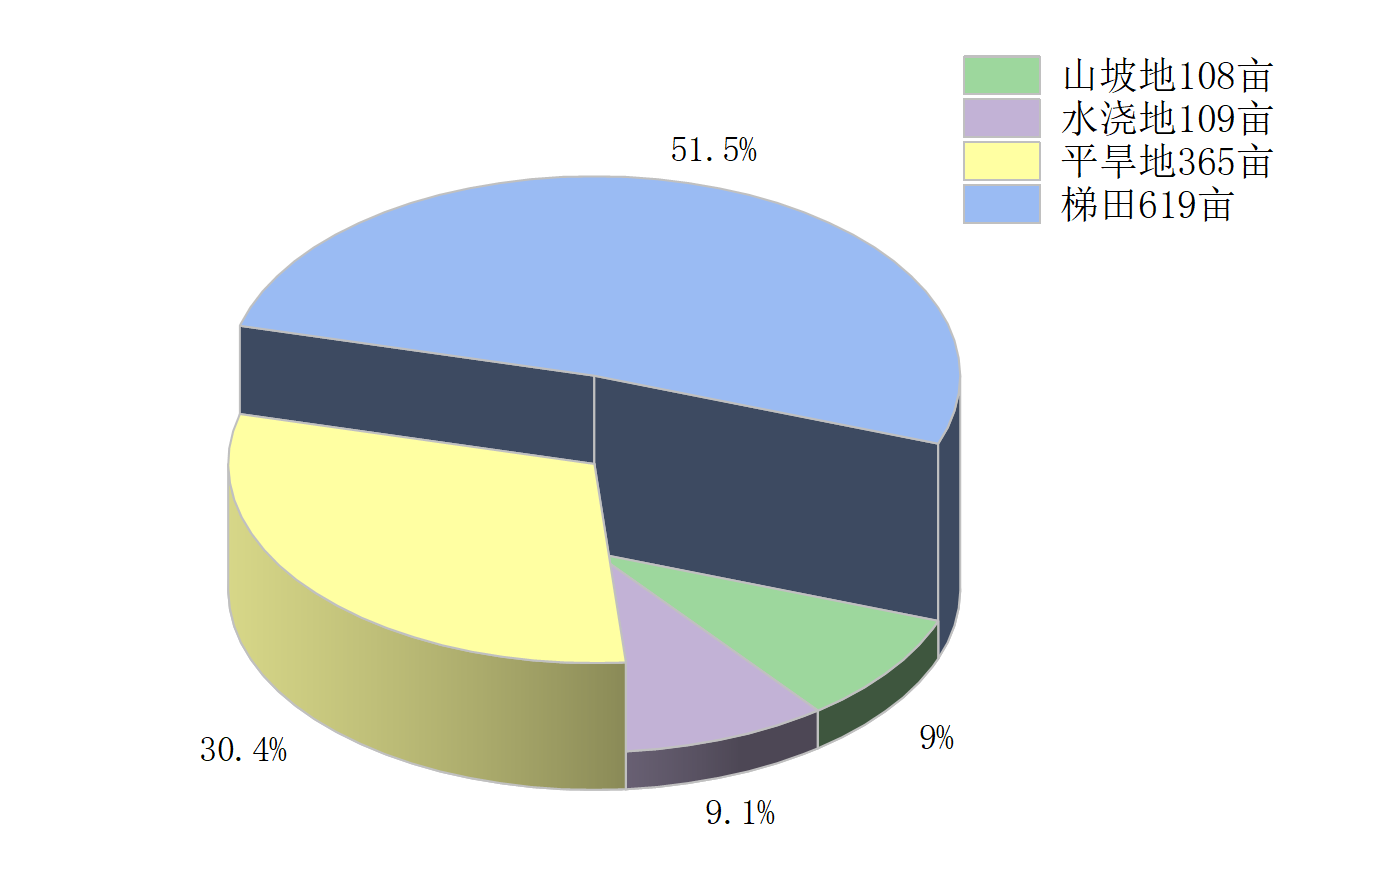
\includegraphics[width=0.6\textwidth]{data/73e4e8516386f2dad5d67adf8b1c943d.png} % 耕地类型占比图
    \caption{耕地类型面积占比}
    \label{fig:land_ratio}
\end{figure}

农作物分为粮食、蔬菜、食用菌三类，种植约束与地块类型强相关，核心约束如表\ref{tab:crop_constraints}所示。
\begin{table}[H]
    \centering
    \caption{农作物类型与种植约束}
    \label{tab:crop_constraints}
    \begin{tabular}{lcl}
    \toprule
    作物类型 & 包含作物 & 核心种植约束 \\
    \midrule
    粮食 & 黄豆、小麦、玉米等 & 平旱地/梯田/山坡地仅单季种植；水浇地可单季种水稻 \\
    蔬菜 & 豇豆、西红柿、大白菜等 & 水浇地可两季种植（第二季限白菜类）；大棚需按季选种 \\
    食用菌 & 榆黄菇、香菇、羊肚菌等 & 仅普通大棚第二季种植（秋冬季） \\
    \bottomrule
    \end{tabular}
\end{table}

\subsection{2023年基础数据统计}
2023年数据为未来预测的基准，关键指标如表\ref{tab:2023_basics}所示（以典型作物为例）。

\begin{table}[H]
    \centering
    \caption{2023年典型作物数据统计}
    \label{tab:2023_basics}
    \begin{tabular}{lcccc}
    \toprule
    作物 & 地块类型 & 亩产量（斤） & 成本（元/亩） & 售价（元/斤） \\
    \midrule
    小麦（粮食） & 平旱地 & 800 & 450 & 3.0-4.0 \\
    豇豆（蔬菜） & 水浇地（第一季） & 3000 & 2000 & 7.0-9.0 \\
    榆黄菇（食用菌） & 普通大棚（第二季） & 5000 & 3000 & 50.0-65.0 \\
    \bottomrule
    \end{tabular}
\end{table}

\subsection{作物总产量分布}
2023年各类作物总产量如图\ref{fig:total_yield}所示，粮食总产量显著高于蔬菜和食用菌，其中小麦、玉米占比最大。

\begin{figure}[H]
    \centering
    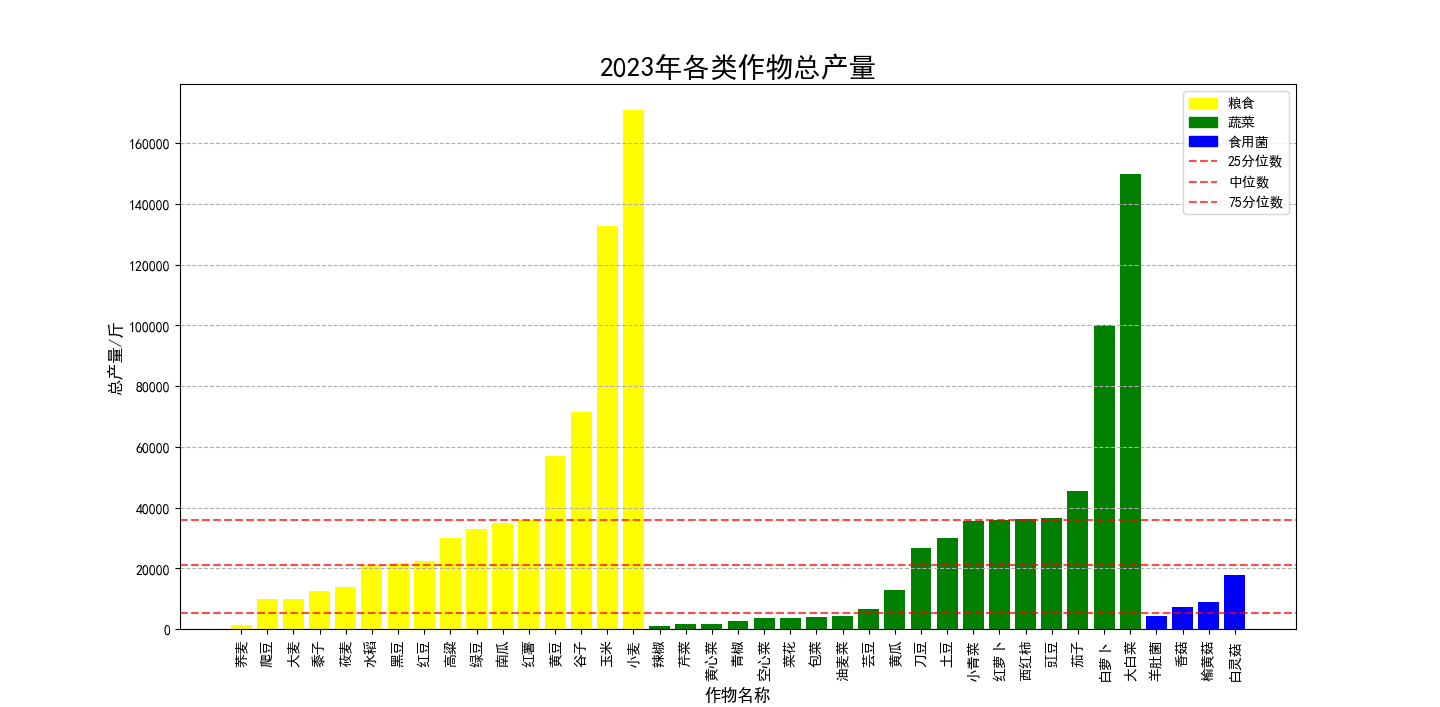
\includegraphics[width=0.8\textwidth]{data/4c18dcb14af1e535c841fd5ed66efc6a.png} % 作物总产量图
    \caption{2023年各类作物总产量分位数分布}
    \label{fig:total_yield}
\end{figure}

\subsection{作物利润对比}
典型作物总利润如图\ref{fig:profit}所示，食用菌（如榆黄菇）利润显著高于蔬菜和粮食，是高附加值作物。

\begin{figure}[H]
    \centering
    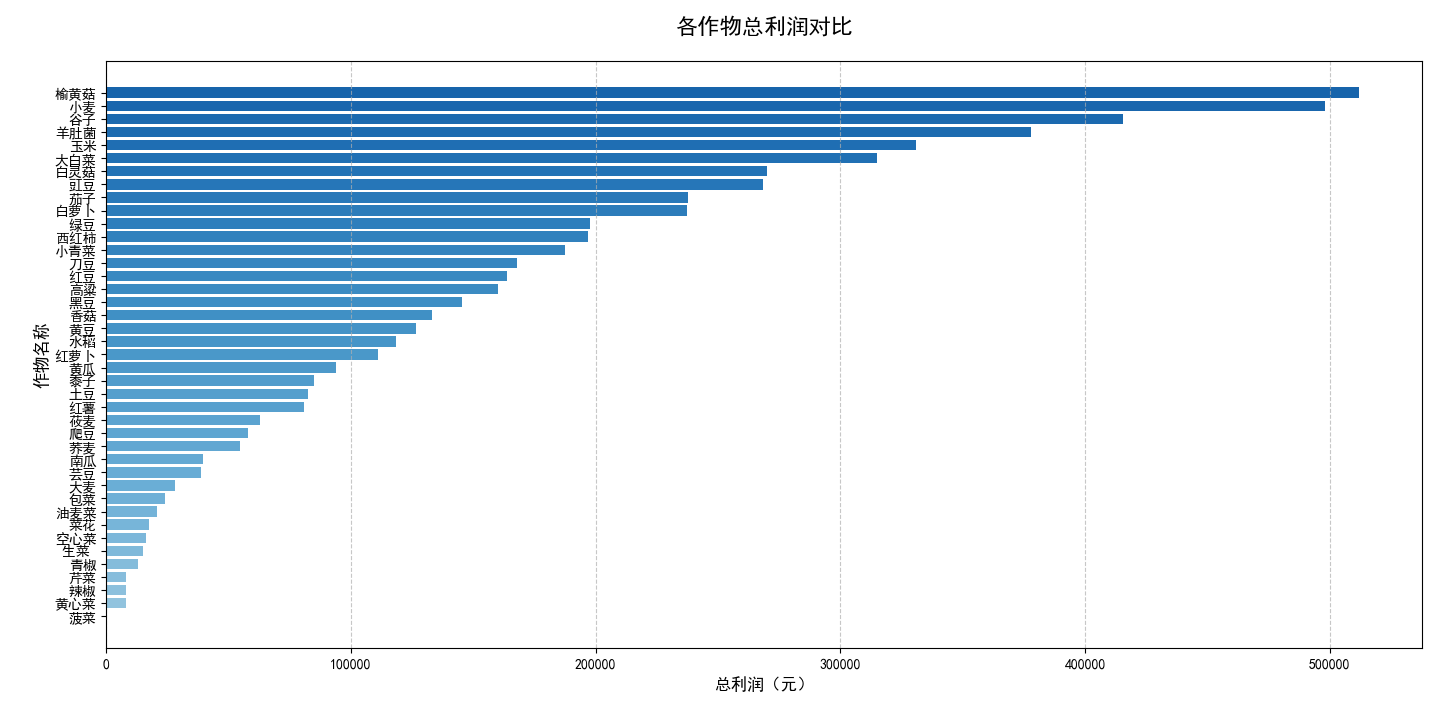
\includegraphics[width=0.6\textwidth]{data/402f23ed9c0cae7d5886011880981b55.png} % 利润对比图
    \caption{2023年各作物总利润对比}
    \label{fig:profit}
\end{figure}

\subsection{大棚资源占比}
智慧大棚与普通大棚面积占比见图\ref{fig:greenhouse_ratio}，普通大棚占比80\%，是食用菌种植的主要载体。

\begin{figure}[H]
    \centering
    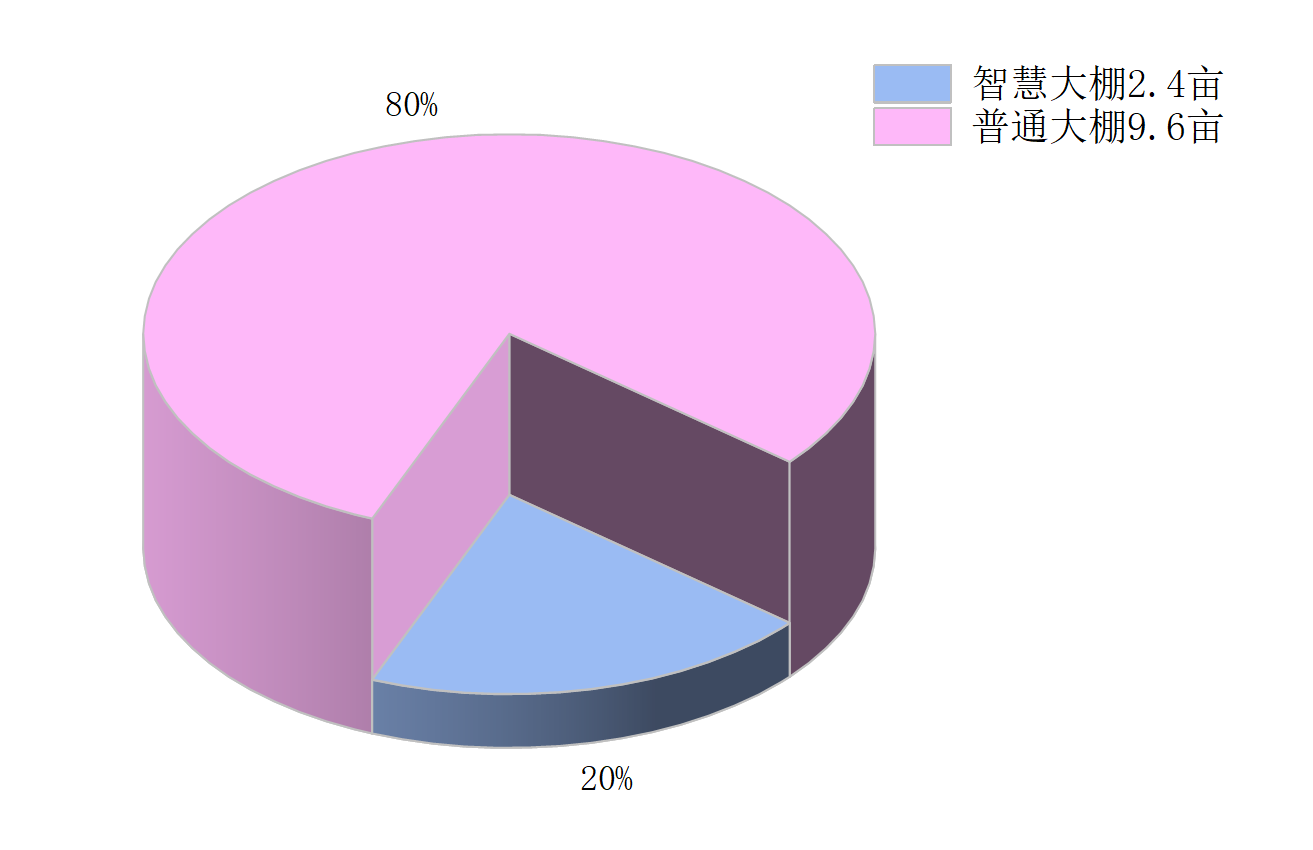
\includegraphics[width=0.4\textwidth]{data/e41e05662d1bb1b0a9d4410a40613337.png} % 大棚占比图
    \caption{大棚类型面积占比}
    \label{fig:greenhouse_ratio}
\end{figure}

预处理后的数据可直接用于构建以利润最大化为目标的线性规划模型，约束条件包括地块面积、轮作要求、销量限制；或引入不确定性参数（如销量增长率、产量波动），采用随机规划或鲁棒优化模型，结合作物替代性调整种植策略。



\section{六、模型建立与求解}
\subsection{6.1 问题一模型建立与求解}
问题一的求解核心在于基于 2023 年固定参数（需求、成本、单产、价格）构建利润最大化模型。输入层采用 2023 年统计数据，其中需求以当年总产量为基准，成本、单产及价格取均值处理（如小麦价格取 3.0-4.0 元 / 斤的均值 3.5 元）。约束体系涵盖地块 - 作物适配性（如平旱地仅第一季可种粮食、普通大棚第二季限种食用菌）、轮作规则（同地块两季禁连作、跨年相邻季禁重茬、三年内至少种植一次豆科作物）及分散度控制（单季单作物种植地块数≤10）。超产处理分为两种情景：（1）超产部分滞销，收入按 “产量≤需求” 计算；（2）超产部分按 50\% 折价销售，收入含折价部分。目标函数为总利润（收入 - 成本）最大化，采用带修复机制的遗传算法（DEAP）求解，通过罚分机制处理约束违反。
\begin{figure}[H]
    \centering
    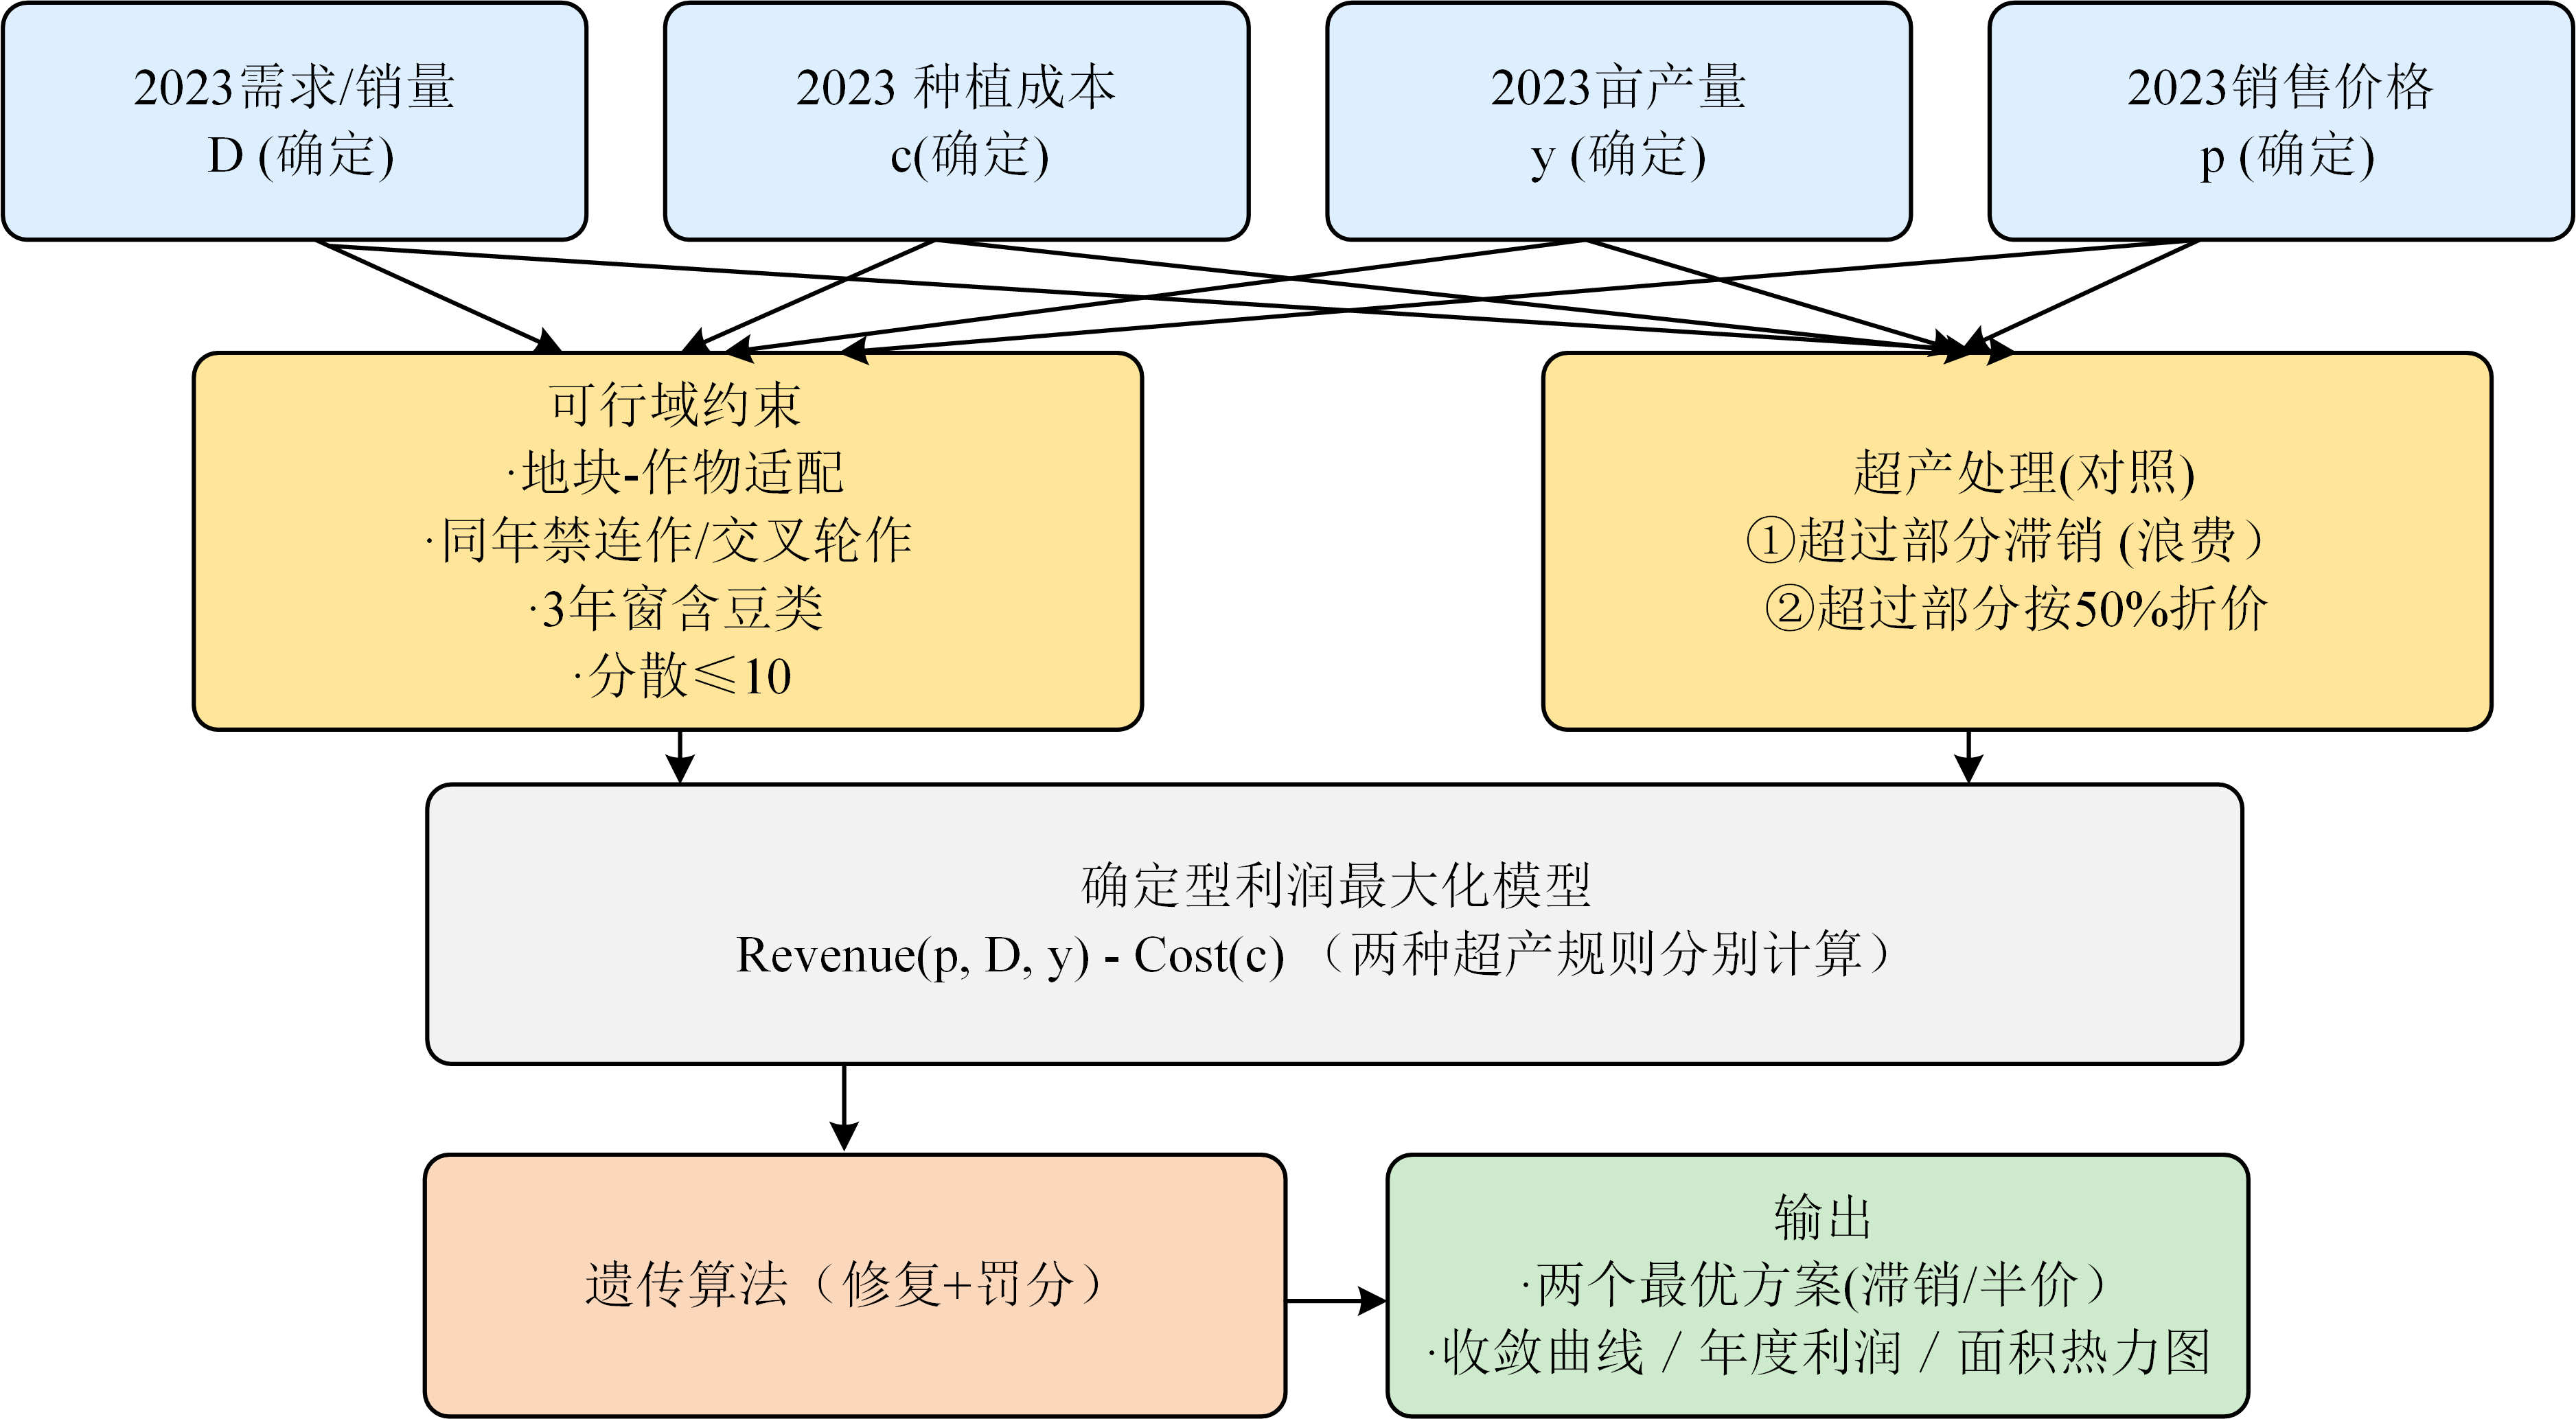
\includegraphics[width=0.8\textwidth]{mindmap/pb1.png} % 耕地类型占比图
    \caption{问题一求解流程图}
    \label{fig:mmp_pb1}
\end{figure}



\subsection{6.1.1 决策变量}
为与实现一致，采用0/1 决策：
\[
z_{\ell y s c}\in\{0,1\},\qquad (\ell,y,s,c)\in \mathcal L\times\mathcal Y\times\mathcal S\times\mathcal C,
\]
表示“地块 $\ell$ 在年份 $y$、季别 $s$ 是否种植作物 $c$”。

\subsection{6.1.2 约束条件}
\textbf{（1）适宜性与单季面积}:
\begin{align}
  &z_{\ell y s c}=0,\quad \forall c\notin \Gamma_{\ell s}; \qquad
  \sum_{c\in\mathcal C} z_{\ell y s c}\le 1, \ \forall \ell,y,s. \label{eq:one-crop-per-season}
\end{align}
若 $z_{\ell y s c}=1$，则该组合在该季占用面积 $a_\ell$。

\textbf{（2）当季产量与年度产量} 作物 $c$ 在年 $y$ 的总产量
\[
P_{cy}=\sum_{\ell\in\mathcal L}\sum_{s\in\mathcal S} a_\ell\, q_c\, z_{\ell y s c}.
\]

\textbf{（3）地块年度耕作最低强度} 每个地块每年至少耕作一季（与实现一致）：
\begin{equation}
\sum_{s\in\mathcal S}\sum_{c\in\mathcal C} z_{\ell y s c}\ \ge 1,\quad \forall \ell,y. \label{eq:at-least-one-season}
\end{equation}
实现中如违反将施加巨额罚分，见ref{sec:algo}。

\textbf{（4）轮作与重茬限制} 
同一地块同年两季不得种同一作物；跨年连续季也不得在同一地块重复同一作物：
\begin{align}
&\sum_{c} z_{\ell y 1 c}\,z_{\ell y 2 c}=0,\quad \forall \ell,y, \\
&\sum_{c} z_{\ell y s c}\,z_{\ell,y+1, s c}=0,\quad \forall \ell,y<2030,\ s\in\{1,2\},\\
&\sum_{c} z_{\ell y,2,c}\,z_{\ell,y+1,1,c}=0,\quad \forall \ell,y<2030.
\end{align}
对应三类“重茬”检测。

\textbf{（5）三年内豆类覆盖} 
任一\,$6$ 个连续季（3 年）内，每个地块至少安排一季豆类作物：
\[
\sum_{\tau=0}^{5}\ \sum_{c\in \mathcal C_{\text{beans}}} z_{\ell, y(\tau), s(\tau), c}\ \ge 1,\quad \forall \ell,\ \forall\ \text{滑动窗口},
\]
其中窗口顺序按“\,$(y,1)\!\to\!(y,2)\!\to\!(y\!+\!1,1)\!\to\!\cdots$”展开。实现中以累计和滑窗检查。

\textbf{（6）同作物当季的地块分散度上限} 
为便于管理，限制任一年—季内任一作物涉及的地块数不超过 $M$（实现取 $M=10$）：
\[
\sum_{\ell\in\mathcal L} z_{\ell y s c}\ \le M,\quad \forall c,y,s.\ \ \ (\text{管理性约束})
\]
违背将受罚。
\subsection{6.1.3 目标函数}
收益按“\emph{不高于需求上限的部分}”计价，超出部分无收入；成本按面积计：
\begin{align}
&\text{收入}\quad R=\sum_{y\in\mathcal Y}\sum_{c\in\mathcal C} p_c\, \min\{P_{cy},\, D_c\},\\
&\text{成本}\quad C=\sum_{y\in\mathcal Y}\sum_{\ell\in\mathcal L}\sum_{s\in\mathcal S}\sum_{c\in\mathcal C} a_\ell\, k_c\, z_{\ell y s c},\\
&\text{目标}\quad \max\ \Pi=R-C.
\end{align}
$D_c$、$q_c$、$p_c$、$k_c$ 均取自 2023 年统计与价格数据的汇总均值。

\subsection{6.1.4 求解方法：遗传算法（GA）}
问题属于多年—多季—多地块—多作物的大规模组合优化。我们采用遗传算法（DEAP 实现）：\\
\textbf{编码}：每个（地块，年，季）为一枚基因，取值为 $\{0,\ldots,|\mathcal C|\}$（0 表示不种，正整数对应作物编号）。不可行（不适宜）的取值在解码时置零。\\
\textbf{适应度}：按上节目标计算 $\Pi$；将违反“至少一季耕作”“禁重茬”“豆类覆盖”“分散度”等约束的个体施加大罚分，使其在进化中被淘汰。\\
\textbf{参数}：种群规模约 240、演化 450 代、两点交叉与均匀变异、锦标赛选择；情景参数取 \texttt{case=waste}（超产无收入）。\\
\textbf{结果回填}：按模板将 2024–2030 年各年两季的（地块$\times$作物）面积矩阵写入 \verb|result1_1.xlsx|。\\
为将\eqref{eq:at-least-one-season}、重茬、豆类覆盖与分散度等约束纳入进化过程，采用大 $M$ 罚分：
\begin{equation}
\label{sec:algo}
\text{Fitness}=\Pi-\underbrace{\big(P_{\text{area}}+P_{\text{rota}}+P_{\text{bean}}+P_{\text{scat}}\big)}_{\text{违反约束的罚分}},
\end{equation}
其中 $P_{\text{area}},P_{\text{rota}},P_{\text{bean}}$ 量级取 $10^7$，$P_{\text{scat}}$ 取 $10^5$，且分散度阈值 $M=10$。参数与检查逻辑与实现保持一致。:contentReference[oaicite:12]{index=12}

\subsection{6.1.5 求解结果与可视化}
算法对 2024–2030 年逐年给出第一季/第二季的地块—作物分配，并按模板在 \verb|result1_1.xlsx| 的各年工作表中写入：若地块 $\ell$ 在年 $y$、季 $s$ 选择作物 $c$，则在该地块行、作物 $c$ 的列填入 $a_\ell(=A_\ell/2)$（亩），从而形成全村在该年该季的面积矩阵。任何违反适宜性、重茬、豆类覆盖或分散度的分配都会在优化过程中被强力淘汰。情景（1）下，模型倾向于\emph{让高单价或高产作物的产出不越过其 $D_c$}，并通过跨年—跨季安排，实现豆类的三年覆盖与避重茬。\hfill
\begin{figure}[htbp]
  \centering
  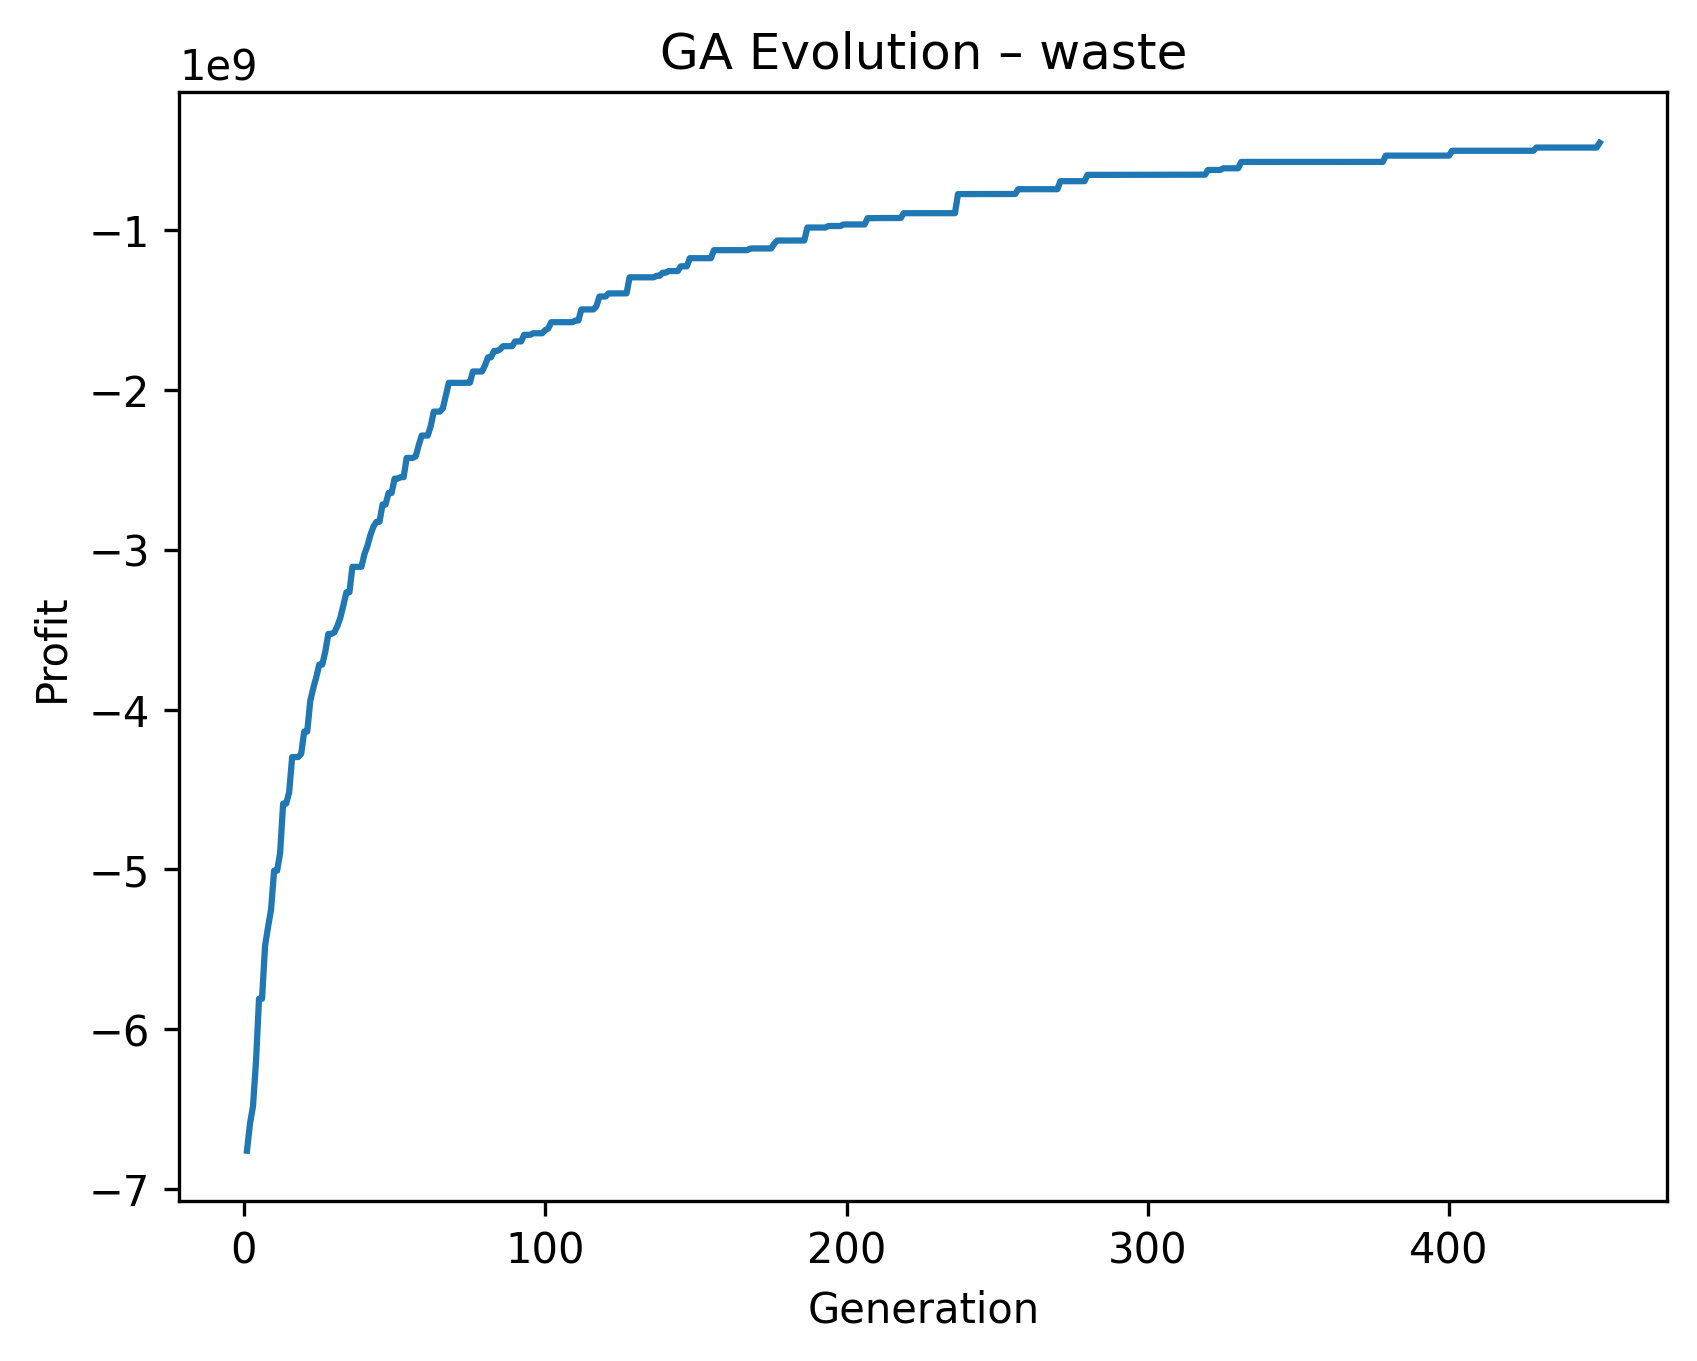
\includegraphics[width=0.70\linewidth]{figure_pb1/problem1_1a.png}
  \caption{超产滞销情况年度利润走势（2024–2030）}
  \label{fig:profit}
\end{figure}
在情景（2）下，优化模型允许超产部分以折扣价出售，提升了有效销售与总利润；GA 求解得到的方案既满足所有适宜性与管理约束，又尽量利用折价销售空间，实现多地块、多作物、多季、多年的全局利润优化。与情景（1）相比，该策略对高需求作物的种植面积配置更为积极，从而减少了浪费并提高了收益。

图\ref{fig:profit} 展示了在情景（1）下 2024–2030 年的年度利润走势；图\ref{fig:evolve} 展示了 GA 在 450 代内的适应度（利润）演化过程，可见前期快速收敛、后期逐步爬升到稳定近优解。

曲线比较平稳，没有特别大的波动，说明模型在每年的产销平衡上控制得较稳定。由于超产不能带来收益，模型会倾向于让各作物产量接近但不超过需求上限，从而避免浪费，这导致年度利润比较平缓。
\begin{figure}[htbp]
  \centering
  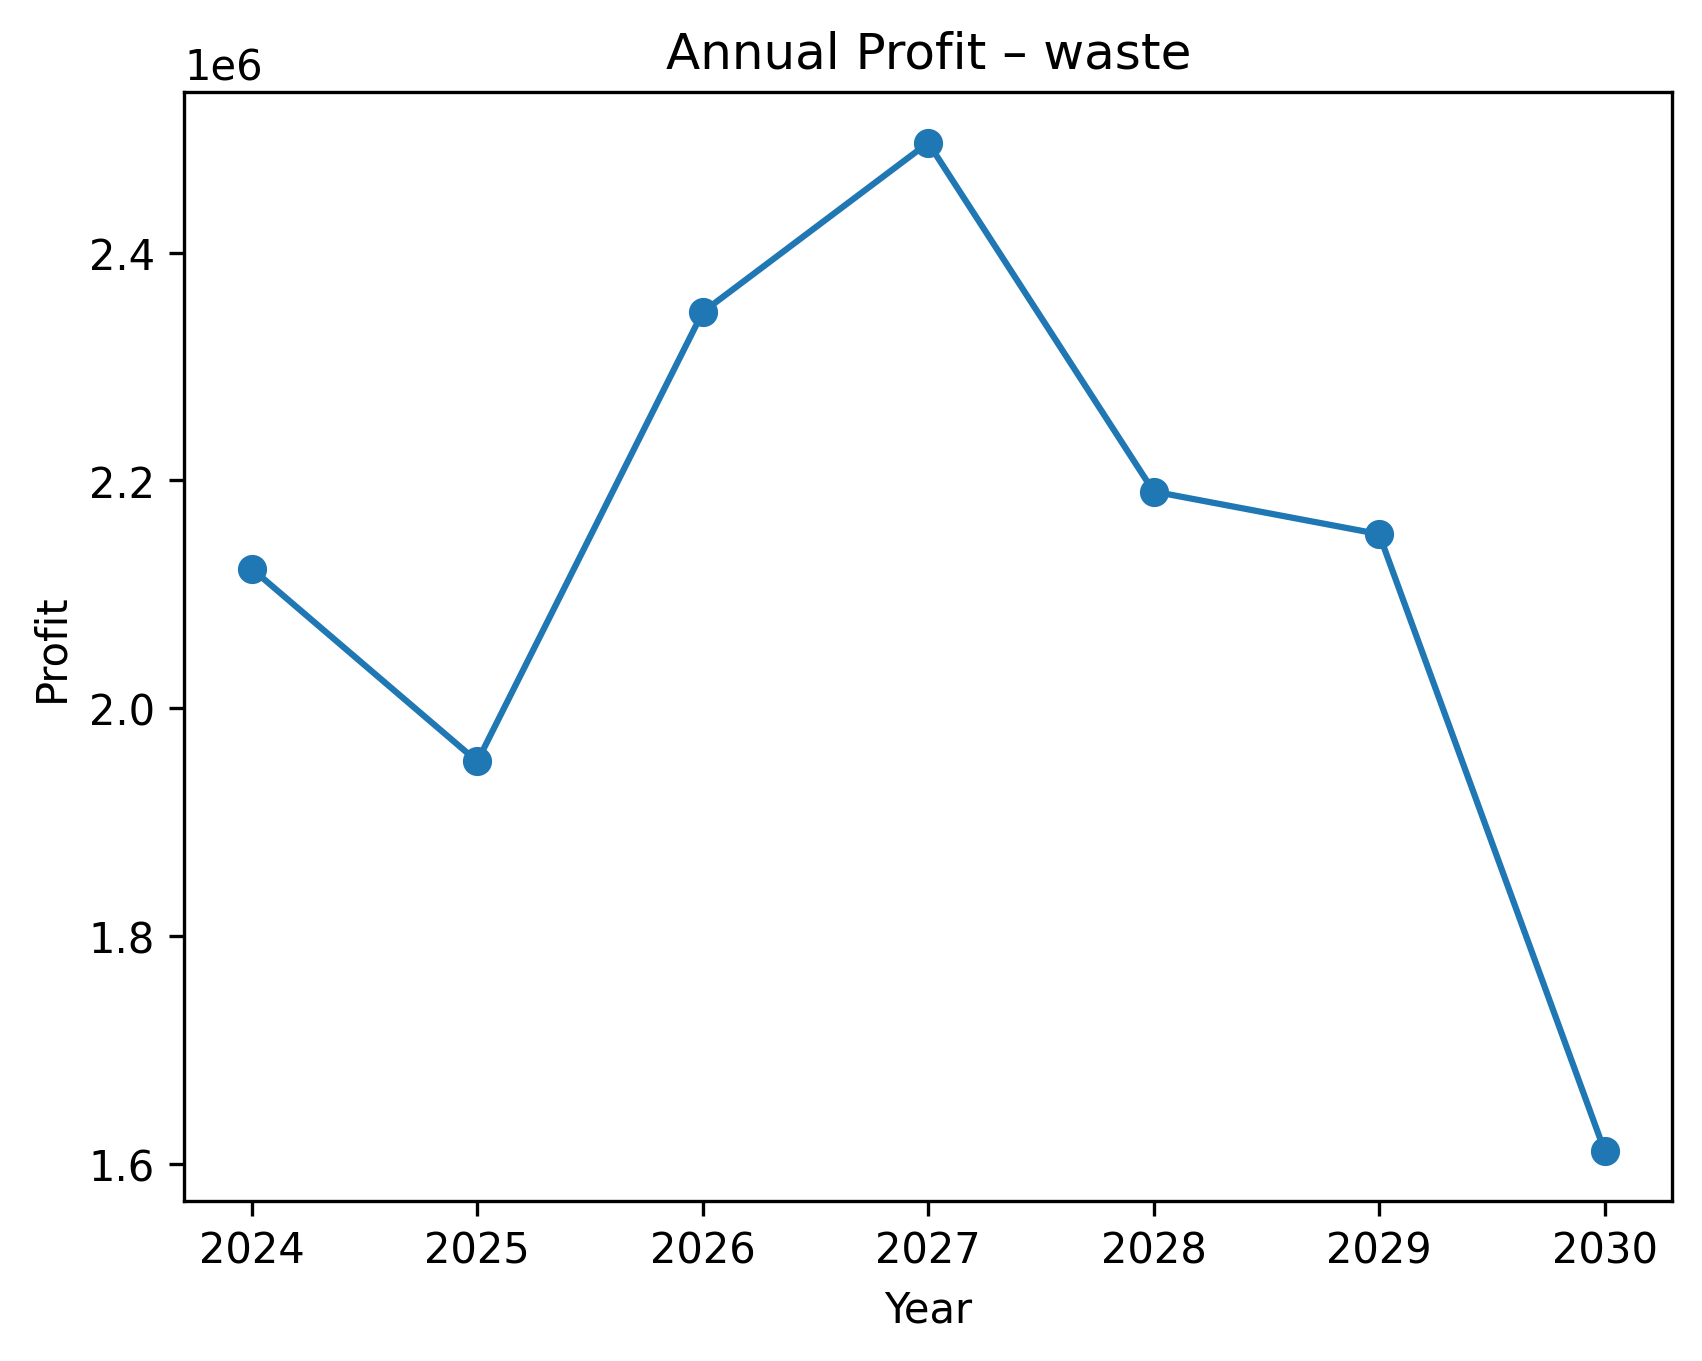
\includegraphics[width=0.70\linewidth]{figure_pb1/problem1_1b.png}
  \caption{超产滞销情况遗传算法演化曲线（情景“超产滞销”）}
  \label{fig:evolve}
\end{figure}
图6曲线一般会快速上升到一个较高水平，然后逐渐趋于平稳，说明算法在前期快速找到较优解，后期进行小幅调整优化。
平稳段的波动很小，说明收敛比较稳定，没有出现大幅震荡。

在“超产滞销”情景下，我们建立了“收益上限截断”的利润最大化模型，并结合可行性掩码与大罚分机制，以遗传算法在多年—多季—多地块—多作物的组合空间内求得满足适宜性、轮作、豆类覆盖与分散度的最优（或近优）方案；结果已按模板输出至 \verb|result1_1.xlsx|。该方案在遵守 agronomic 约束的前提下，最大化了可售产出的收益并抑制了超产浪费。
图\ref{fig:profit_discount} 显示了情景（2）下 2024–2030 年的年度利润走势；图\ref{fig:evolve_discount} 给出了遗传算法在 450 代内的演化曲线。

\begin{figure}[htbp]
  \centering
  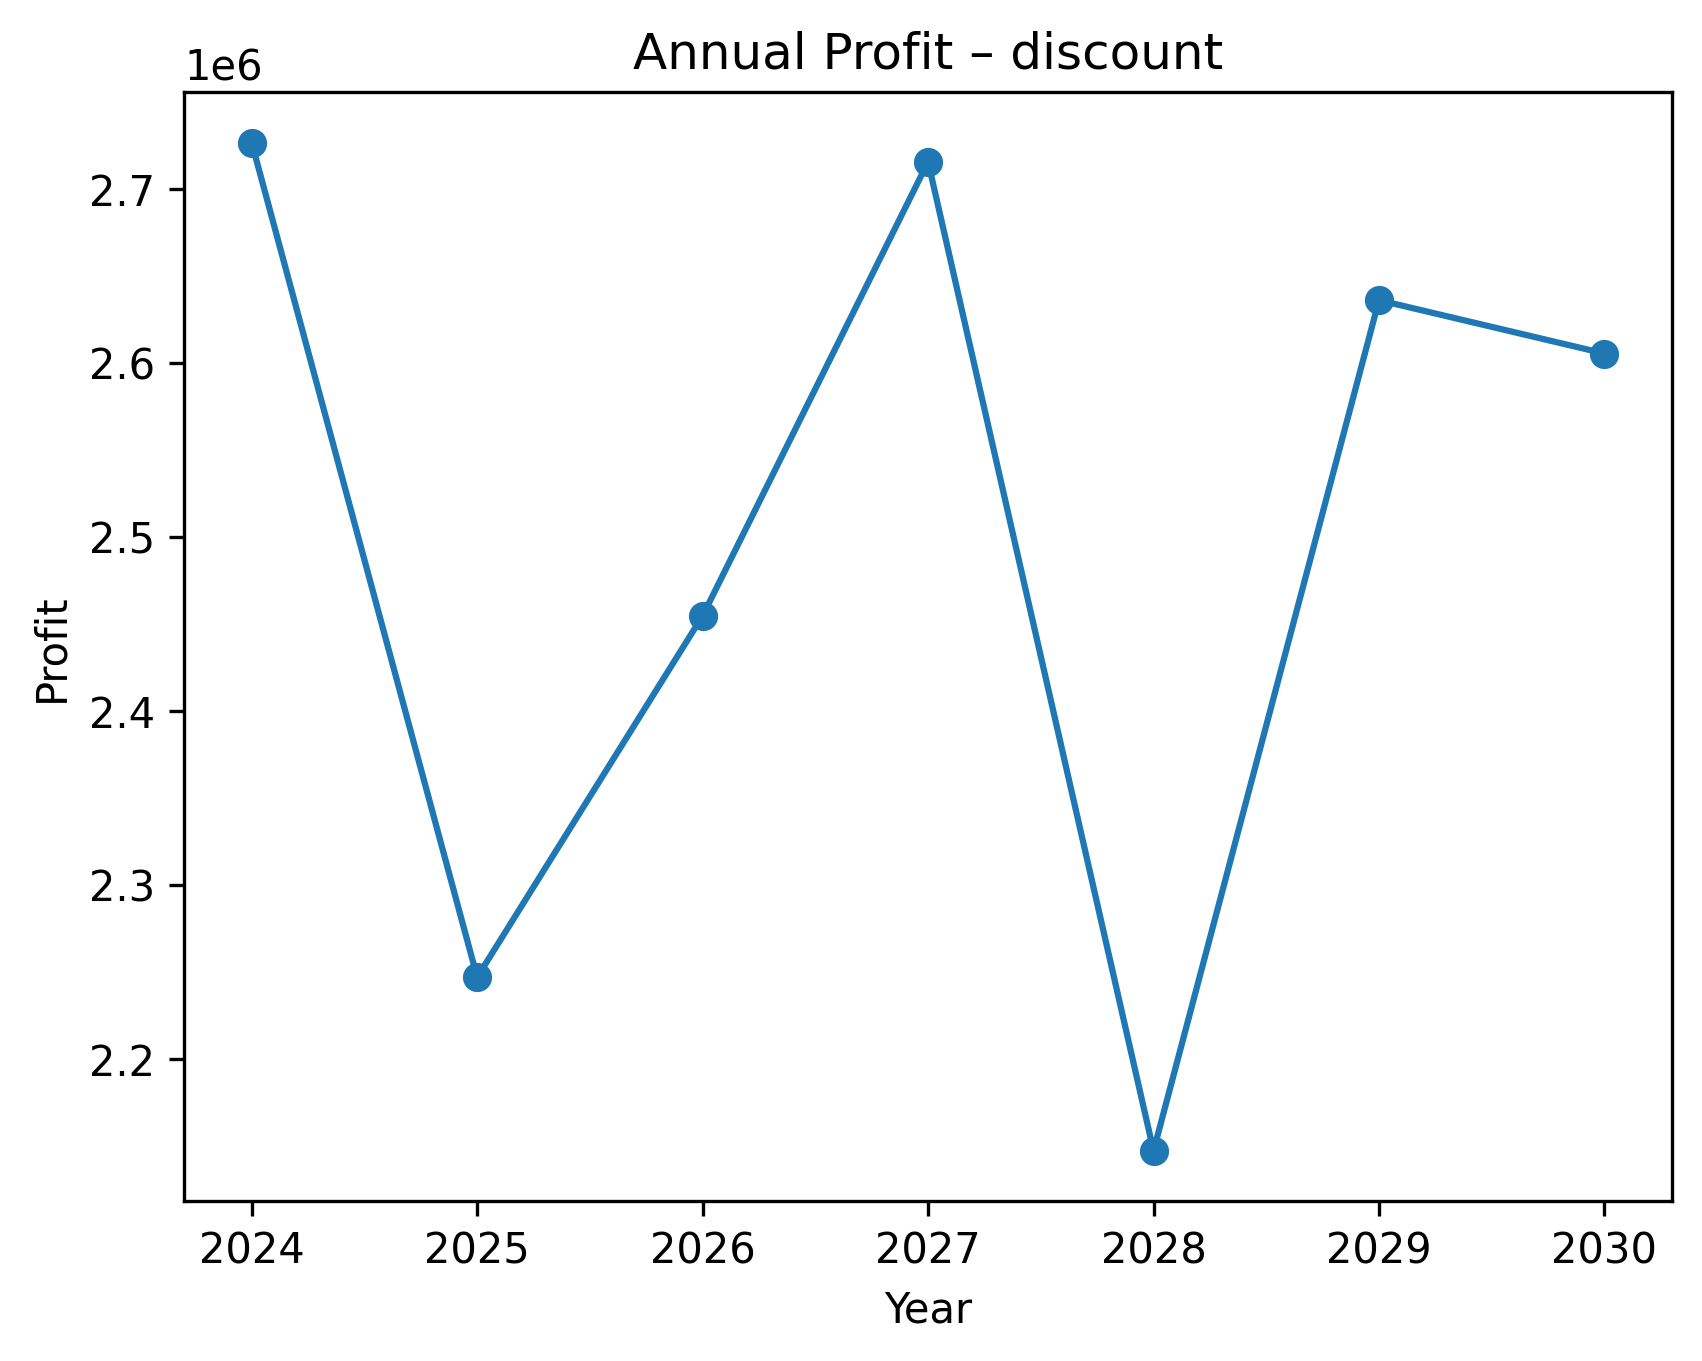
\includegraphics[width=0.70\linewidth]{figure_pb1/discount_years (1).png}
  \caption{情景（2）年度利润走势（2024–2030）}
  \label{fig:profit_discount}
\end{figure}

\begin{figure}[htbp]
  \centering
  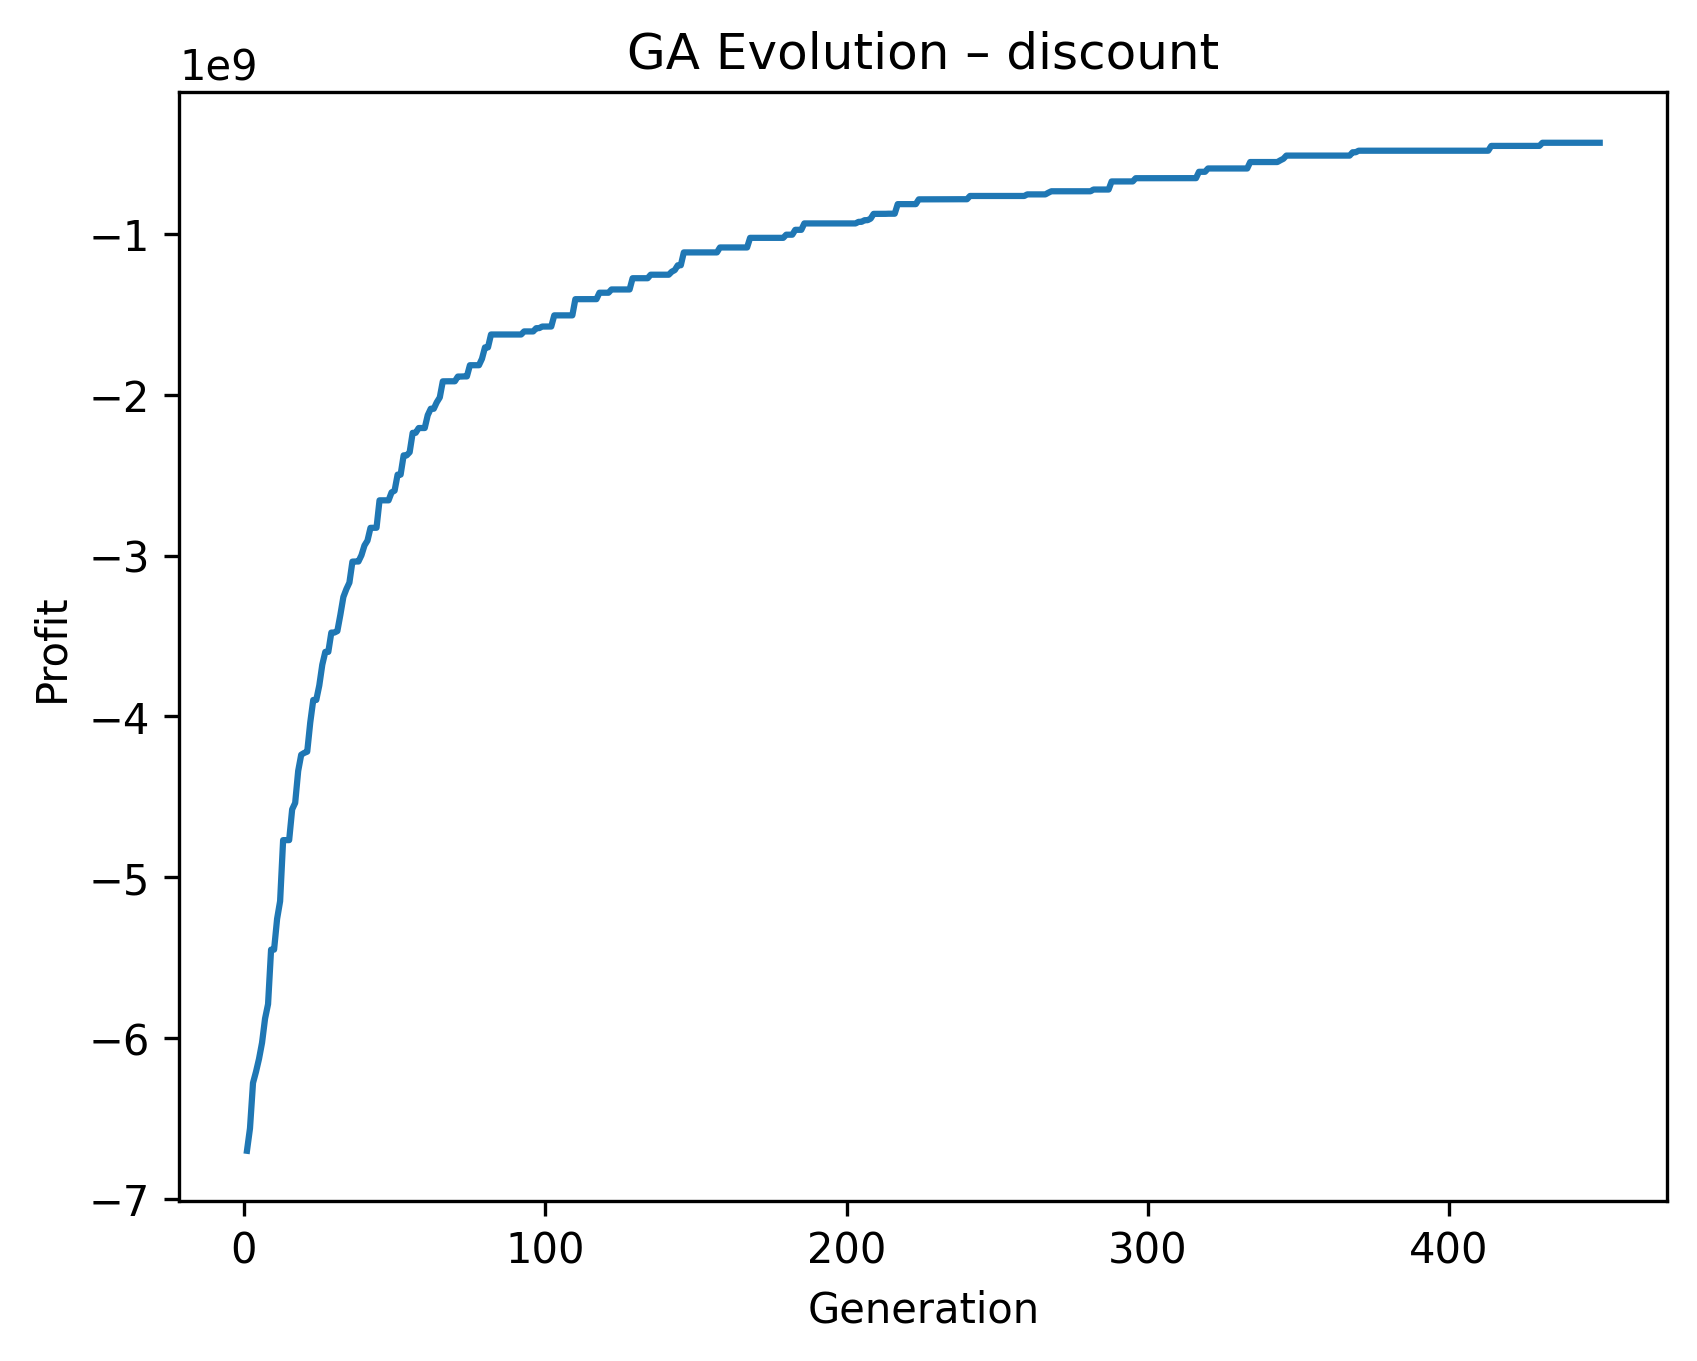
\includegraphics[width=0.70\linewidth]{figure_pb1/discount_evolve.png}
  \caption{遗传算法演化曲线（情景“超产折价”）}
  \label{fig:evolve_discount}
\end{figure}
与“滞销”情景相比，这里的利润整体水平更高，因为超产部分虽然不能按原价卖出，但可以以 50\% 的价格出售，从而带来额外收益。
曲线可能比滞销情景略有波动，尤其在某些年份高利润作物种植面积增加、折价销售比例较高时，总利润会有所变化。

迭代代数与适应度的变化趋势与滞销情景类似，但收敛的最终值更高。
前期快速上升，说明模型在折价销售条件下，能迅速找到比滞销情景更高的利润方案。
后期波动幅度稍大，可能是因为折价销售策略增加了种植配置的灵活性，使得解空间更大。




\subsection{6.2 问题二模型建立与求解}

在问题二中，我们在保持问题一可行域约束不变的前提下，引入了需求、产量、成本与价格等市场与生产参数的年际波动，将其建模为随机变量，并通过多情景仿真刻画不确定性影响。首先，根据题设区间或波动范围对预期销量、亩产量、种植成本及销售价格进行采样，生成多条完整的 2024--2030 年参数路径。在每个情景下，利用超产折价销售规则计算年度总利润，并将利润不足部分定义为 Shortfall 损失 $L = \max(I - \Pi, 0)$，进一步在置信度 $\alpha=0.95$ 下计算条件在险价值 $\mathrm{CVaR}_\alpha(L)$ 作为极端风险度量。优化目标采用均值--风险权衡形式 $\max E[\Pi] - \lambda \cdot \mathrm{CVaR}_\alpha(L)$，通过遗传算法在多情景利润分布下迭代寻优，得到兼顾收益与稳健性的种植方案，并输出期望利润与风险指标，用于构建风险--收益前沿与年度面积配置方案。

\begin{figure}[H]
    \centering
    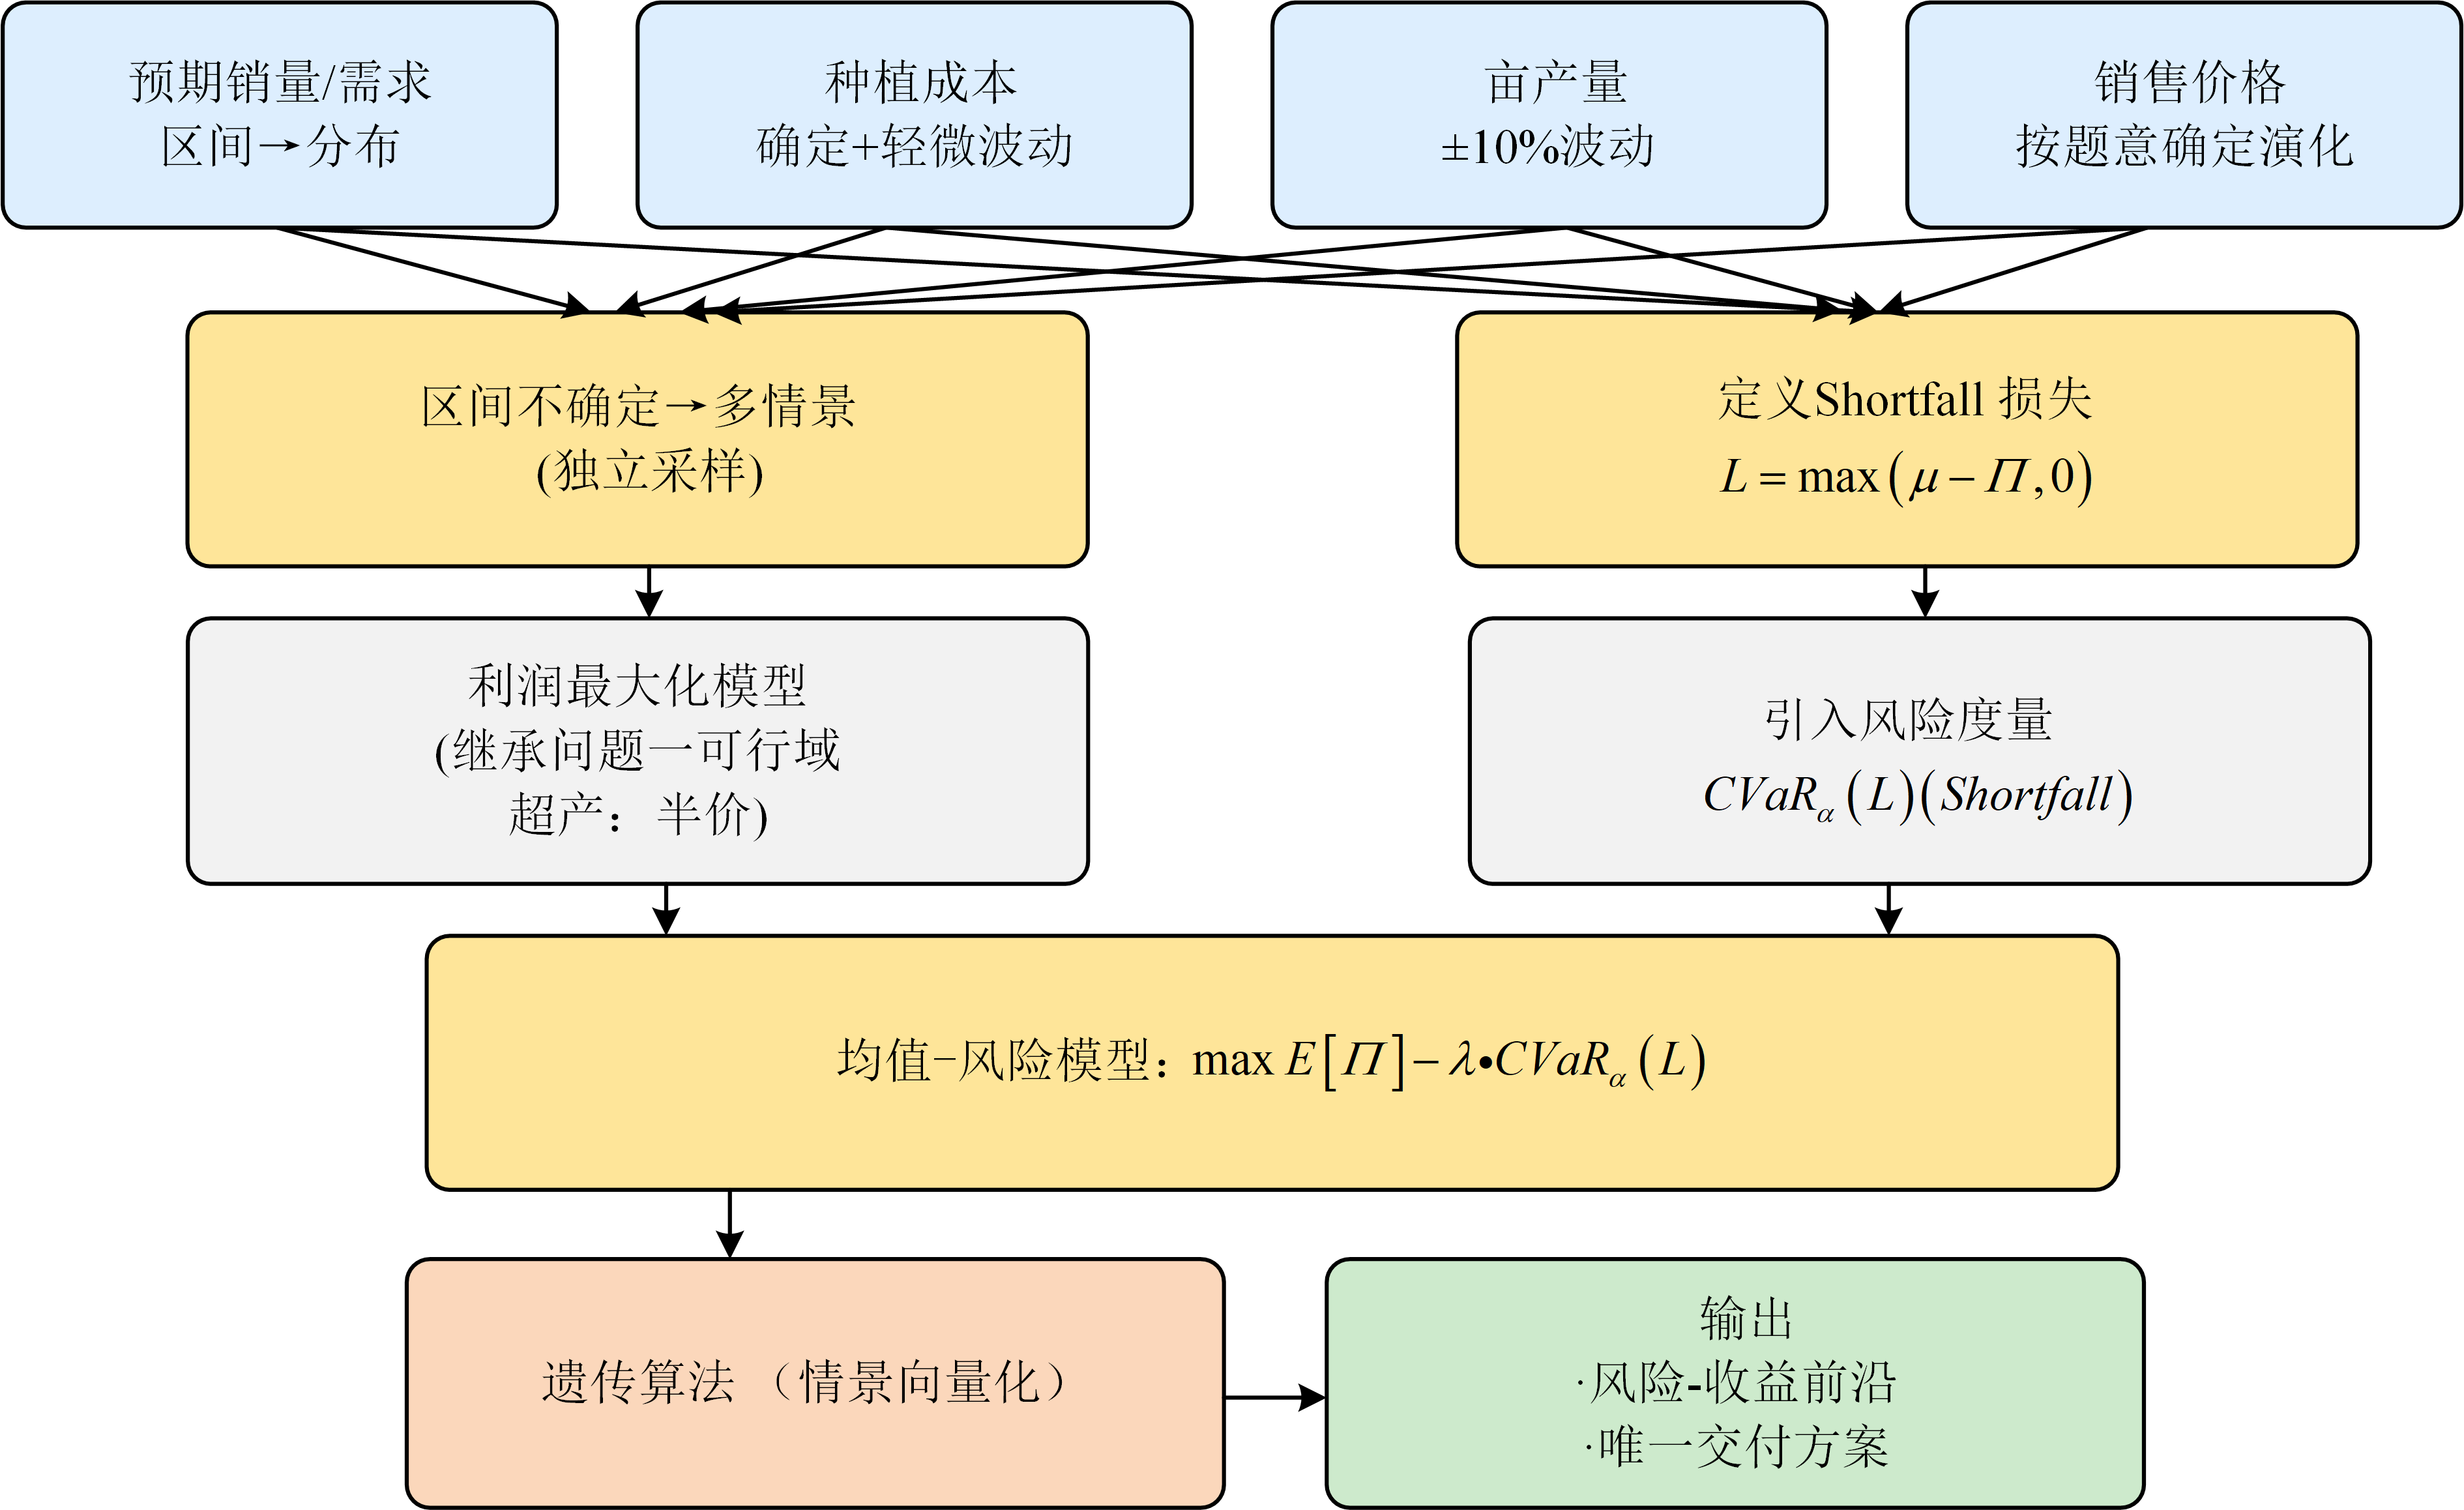
\includegraphics[width=0.8\textwidth]{mindmap/pb2.png} % 耕地类型占比图
    \caption{问题二求解流程图}
    \label{fig:mmp_pb2}
\end{figure}
在问题二中，我们在保留问题一可行域约束（地块适宜性、轮作重茬、三年豆类覆盖率、作物分散度等）的基础上，仅将赛题中给出具有区间波动或年变化趋势的参数建模为随机变量，其余参数保持为确定值，具体处理方式如下：
小麦与玉米年增长率 $g_{wc} \sim U(0.05, 0.10)$，即 $D_{c,y} = D_{c,2023} \cdot (1+g_{wc})^{y-2023}$；其他作物年变动率 $\epsilon \sim U(-0.05, 0.05)$，即 $D_{c,y} = D_{c,2023} \cdot (1+\epsilon)$。
亩产量年波动率 $\delta \sim U(-0.10, 0.10)$，则 $q_{c,y} = q_{c,2023} \cdot (1+\delta)$。
种植成本年通胀率 $r_{\text{inf}} \sim U(0.03, 0.07)$，成本随年份累积增长，即 $k_{c,y} = k_{c,2023} \cdot \prod_{\tau=2024}^{y} (1+r_{\text{inf},\tau})$。
对于销售价格, 粮食类作物价格稳定，$p_{c,y} = p_{c,2023}$；蔬菜类作物：设年增长率为 $5\%$，即 $p_{c,y} = p_{c,2023} \cdot 1.05^{y-2023}$；食用菌类作物年下降率 $r_{\text{fungi}} \sim U(0.01,0.05)$，即 $p_{c,y} = p_{c,2023} \cdot \prod_{\tau=2024}^{y} (1-r_{\text{fungi},\tau})$；其中羊肚菌固定下降 $5\%$/年。
以上随机变量在多情景仿真中独立采样生成，形成2024--2030 年的完整参数路径。超额产出按当年售价的 $50\%$ 折价销售。

\subsection{6.2.1 决策变量}
决策采用地块—年—季—作物四维 0-1 变量
\[
z_{\ell y s c}\in\{0,1\},\qquad (\ell\in\mathcal L,\ y\in\mathcal Y,\ s\in\mathcal S,\ c\in\mathcal C),
\]
表示是否在 $(\ell,y,s)$ 种植作物 $c$。实现中以\emph{整数基因编码}并在解码时用\emph{可行性掩码}过滤不适宜的地块类型—季别—作物组合。
\subsection{6.2.2 收益、成本与风险口径}
在场景 $\omega$、年份 $y$ 下，作物 $c$ 的产量与收入为
\[
P_{c,y}=\sum_{\ell\in\mathcal L}\sum_{s\in\mathcal S} a_{\ell s}\, q_{c,y}^{(\omega)}\, z_{\ell y s c},\qquad
R_{c,y}^{(\omega)}=p_{c,y}^{(\omega)}\!\cdot\!\min\!\{P_{c,y},D_{c,y}^{(\omega)}\}+0.5\,p_{c,y}^{(\omega)}\!\cdot\!\max\!\{0,P_{c,y}-D_{c,y}^{(\omega)}\}.
\]
对应的成本
\[
C_{y}^{(\omega)}=\sum_{\ell,s,c} a_{\ell s}\,k_{c,y}^{(\omega)}\,z_{\ell y s c},\qquad
\Pi^{(\omega)}=\sum_{y,c} R_{c,y}^{(\omega)}- \sum_y C_{y}^{(\omega)}.
\]
为抑制尾部亏损，采用\textbf{条件在险价值}（CVaR）约束目标。设置信度 $\alpha=0.95$，记损失 $L^{(\omega)}=-\Pi^{(\omega)}$，则
\[
\text{CVaR}_\alpha(L)=\mathbb{E}\!\left[L^{(\omega)}\mid L^{(\omega)}\ge \text{VaR}_\alpha(L)\right].
\]
问题二的\emph{风险—收益权衡}目标为
\[
\max\ \ \mathbb{E}_\omega[\Pi^{(\omega)}]\ -\ \lambda\cdot \text{CVaR}_{0.95}\!\big(L^{(\omega)}\big),
\]
其中 $\lambda$ 为权重（默认 $\lambda=0.10$）。实现中以\emph{样本平均}估计 $\mathbb{E}[\cdot]$，并以\emph{分位截尾均值}估计 CVaR。

\subsection{6.2.3 问题二求解过程：情景—遗传算法（Scenario--GA）} 
\noindent \textbf{场景生成} 按设定随机生成 $N=300$ 条 2024--2030 的参数路径（需求、亩产、价格、成本）并缓存为张量 \texttt{DEMAND}, \texttt{YIELD}, \texttt{PRICE}, \texttt{COST}; \\
\textbf{编码与解码} 个体长度 $|\mathcal L|\times|\mathcal Y|\times 2$（两季），整数基因 $\{0,\ldots,|\mathcal C|\}$；解码时应用可行性掩码 \texttt{compat} 将非法作物置零;  \\
\textbf{适应度评估} 向量化计算所有场景利润 $\Pi^{(\omega)}$，减去罚分并据此计算 $\mathbb{E}[\Pi]-\lambda\cdot \text{CVaR}_{0.95}(L)$ 作为适应度；  \\
\textbf{演化参数} 锦标赛选择、两点交叉（概率 $0.8$）、均匀变异（\texttt{indpb}$=0.03$），种群规模 $240$、迭代 $450$ 代；  \\
\textbf{结果输出} 最优个体写回 \verb|result2.xlsx|（各年工作表、两季分区，按“地块行 × 作物列”填入面积)。

\subsection{6.2.4 求解结果与可视化}
\paragraph{输出口径} 代码将 2024--2030 年的地块—作物面积矩阵写入 \verb|result2.xlsx|；同时打印\emph{经济期望利润}与\emph{CVaR95\%（亏损）}等指标，便于与不同 $\lambda$、不同场景数 $N$ 做稳健性对比。

\begin{figure}[htbp]
  \centering
  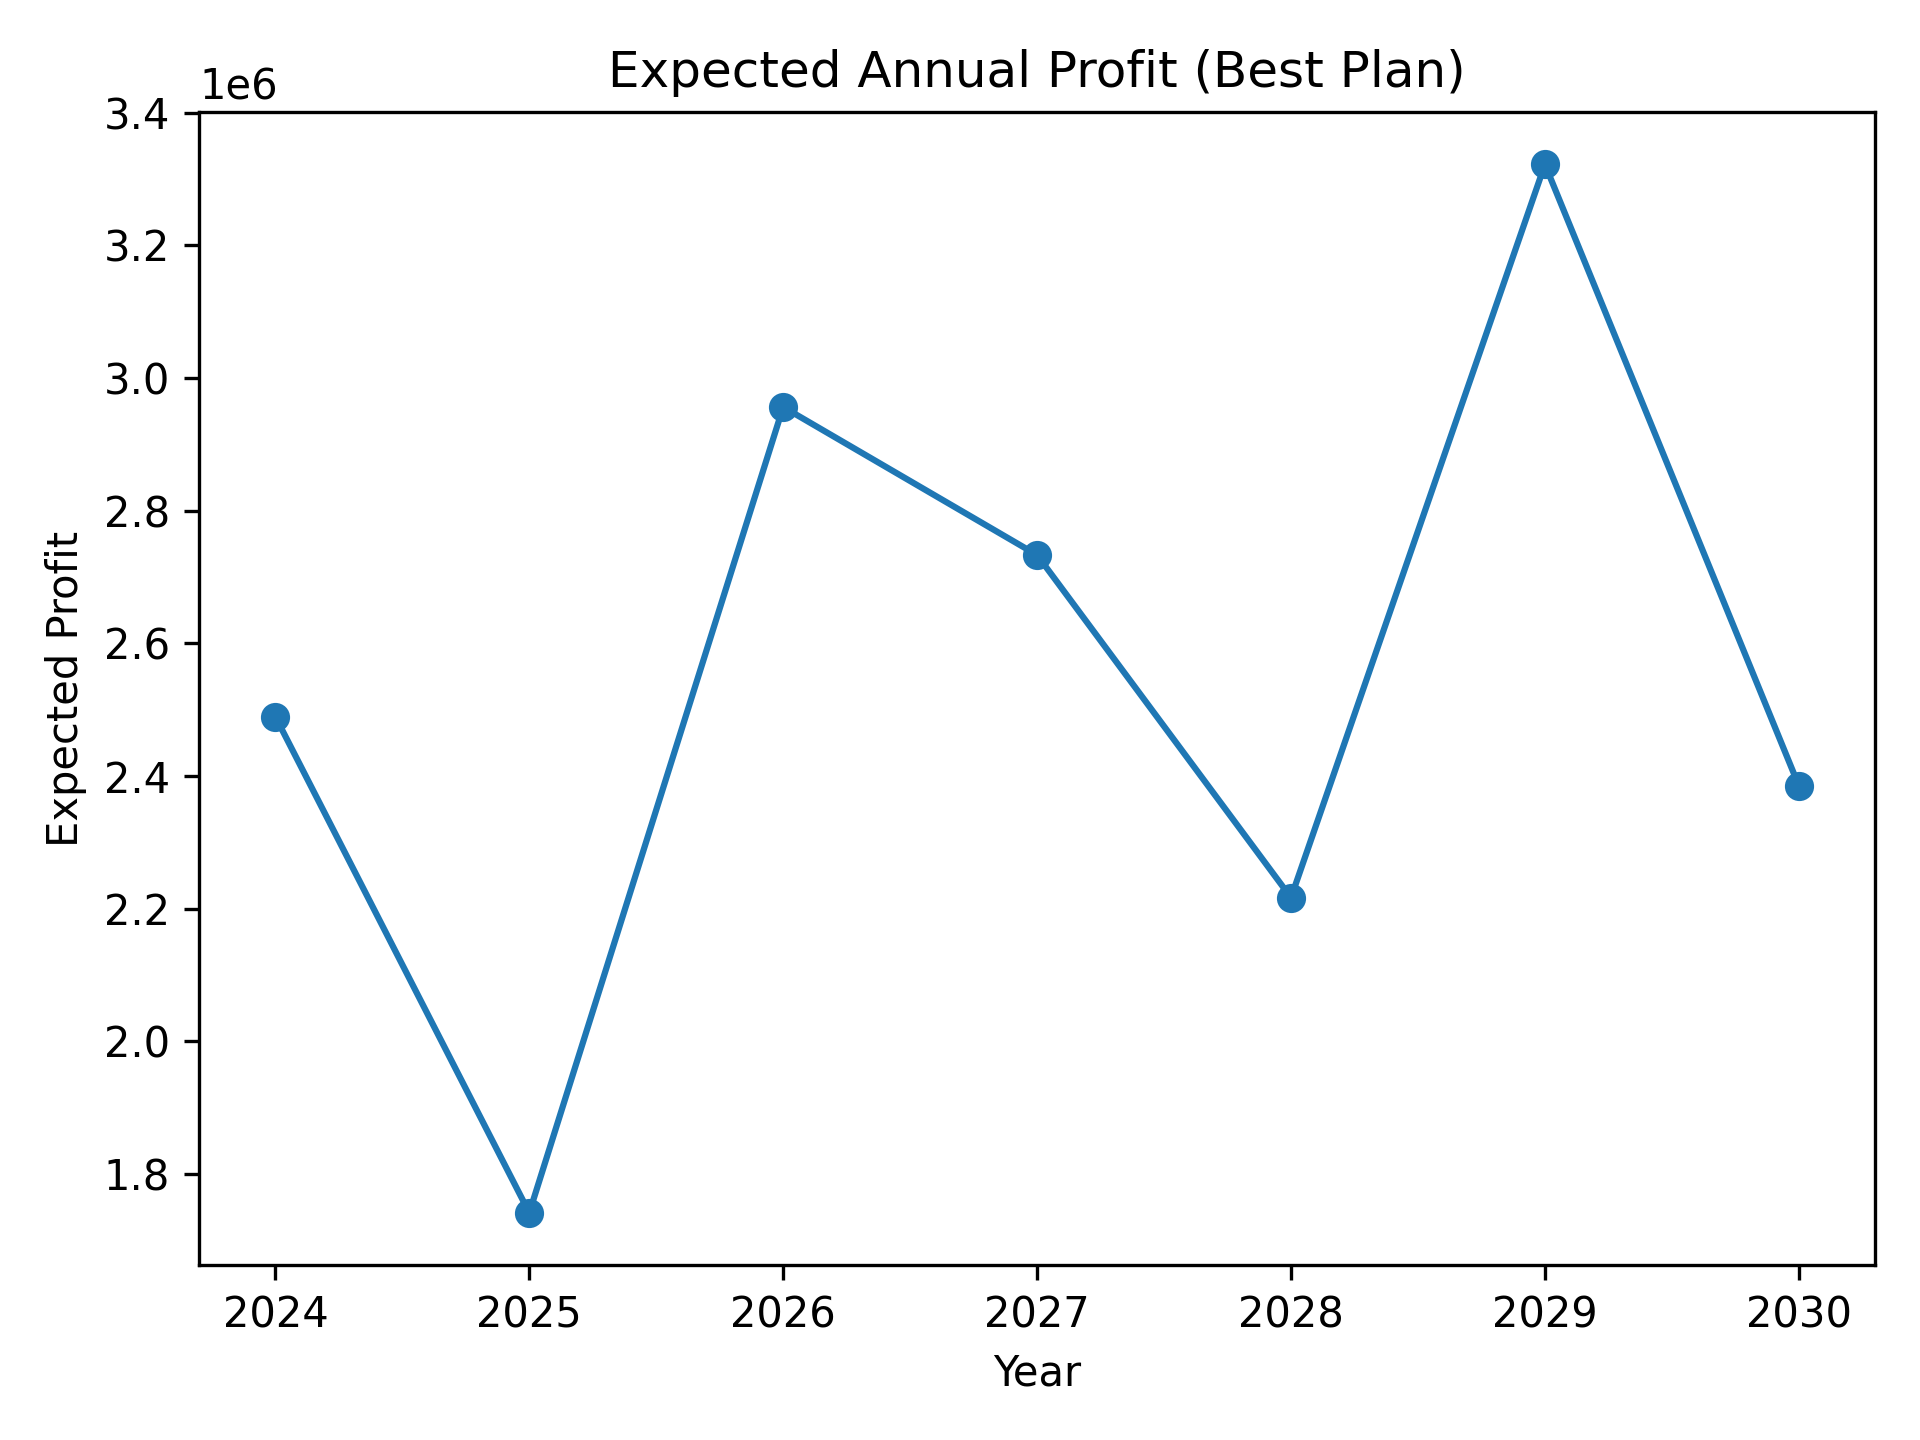
\includegraphics[width=0.85\linewidth]{figure_pb2/52bbcae1b8a57b4d8419f18e54723e59.png}
  \caption{问题二情景下最优方案的年度期望利润（2024--2030）}
  \label{fig:profit_q2}
\end{figure}

图\ref{fig:profit_q2} 展示了在考虑销量、产量、价格、成本等不确定性以及折价销售与风险惩罚后的\textbf{年度期望利润}。年度利润在不同年份间存在波动，其中 2025 年出现显著低谷，可能由不利的市场与产量情景叠加引起；,2029 年利润达到峰值，说明当年作物结构与市场条件的匹配度高,利润波动反映了模型在不同年度对高风险作物的适度回避与结构调整，这是 CVaR 风险约束作用的结果。

\begin{figure}[htbp]
  \centering
  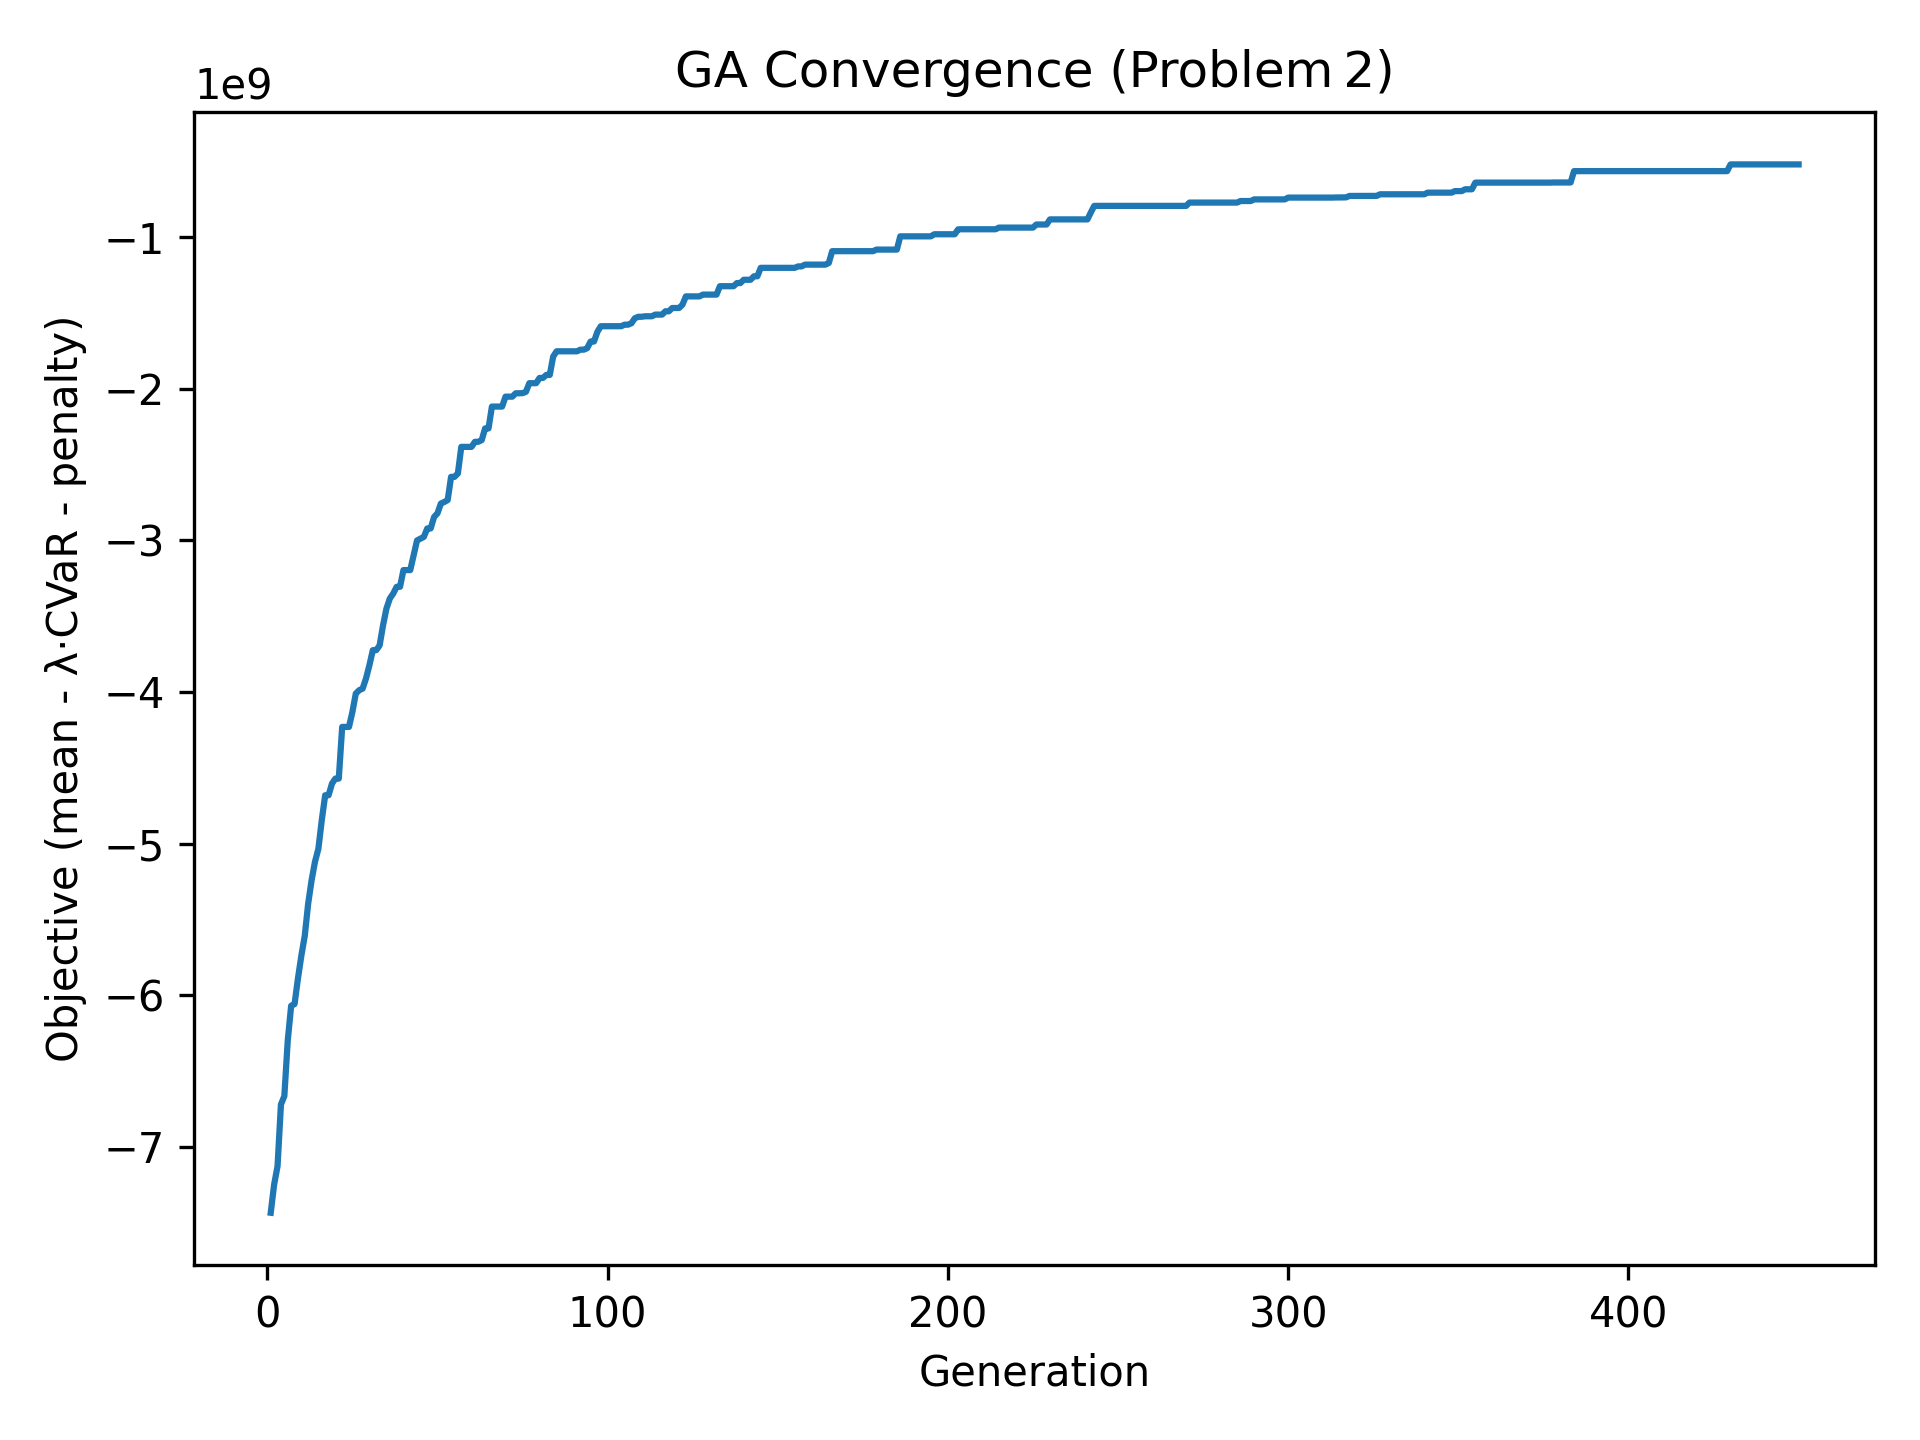
\includegraphics[width=0.85\linewidth]{figure_pb2/7a60f47d3ac8127fa0170bac7a863a80.png}
  \caption{遗传算法在问题二中的收敛过程}
  \label{fig:ga_q2}
\end{figure}

图\ref{fig:ga_q2} 显示了遗传算法在 450 代迭代中的\emph{目标值}变化情况，目标值定义为
\[
\mathbb{E}[\Pi] - \lambda\cdot\text{CVaR}_{95\%}(\text{亏损}) - \text{罚分}.
\]

优化模型的目标函数值：
\begin{equation}
\mathrm{Objective} = \mathbb{E}[\Pi(\omega)] - \lambda \cdot \mathrm{CVaR}_{0.95}(L) - \mathrm{Penalty},
\end{equation}
其中 $\mathbb{E}[\Pi(\omega)]$ 表示多情景下的平均利润，$\mathrm{CVaR}_{0.95}(L)$ 为最差 $5\%$ 场景下亏损的条件期望，$\lambda$ 为风险权重系数；Penalty 为约束罚分，包括地块适宜性、轮作重茬、三年豆类覆盖率以及作物分散度等硬性约束的惩罚项，其量级高达 $10^7$ 元。\\
优化模型的目标函数值：
\begin{equation}
\mathrm{Objective} = \mathbb{E}[\Pi(\omega)] - \lambda \cdot \mathrm{CVaR}_{0.95}(L) - \mathrm{Penalty},
\end{equation}
其中 $\mathbb{E}[\Pi(\omega)]$ 表示多情景下的平均利润，$\mathrm{CVaR}_{0.95}(L)$ 为最差 $5\%$ 场景下亏损的条件期望，$\lambda$ 为风险权重系数；Penalty 为约束罚分，包括地块适宜性、轮作重茬、三年豆类覆盖率以及作物分散度等硬性约束的惩罚项，其量级高达 $10^7$ 元。该设计旨在使严重违反约束的解在进化过程中被快速淘汰。

在演化初期，种群中大多数个体不仅经济利润较低，还存在严重的约束违反，导致罚分总额和风险惩罚项远大于利润值，从而使目标函数呈现大幅负值。随着迭代推进，遗传算法逐步修复不可行解，降低罚分并改善收益--风险平衡，目标函数值快速上升并趋于稳定。因此，纵坐标的负值仅反映了优化早期约束违反程度与风险水平较高的状态，并不意味着种植方案在经济上亏损。在演化初期，种群中大多数个体不仅经济利润较低，还存在严重的约束违反，导致罚分总额和风险惩罚项远大于利润值，从而使目标函数呈现大幅负值。随着迭代推进，遗传算法逐步修复不可行解，降低罚分并改善收益--风险平衡，目标函数值快速上升并趋于稳定。

结合两幅图可知，最终的最优种植方案在多数年份保持了较高的期望利润，并有效降低了极端亏损风险。这表明风险约束促使模型在高收益与稳健性之间取得平衡,遗传算法在此多情景、多约束的复杂组合优化中具有良好的收敛性与稳定性。


\subsection{6.3 问题三：相关性与替代/互补性下的最优种植策略}
在问题二的基础上，问题三进一步考虑了\textbf{农作物之间的相关性}以及\textbf{替代性/互补性}，并将其引入到多情景风险优化模型中。为此，构建了销量（D）、价格（P）、成本（C）三类变量的相关矩阵，通过 Copula 方法生成相关随机情景,突破独立情景假设，并结合交叉价格弹性系数，对需求进行价格联动修正，最后在相同农艺与管理约束下使用遗传算法（GA）进行求解,输出优化方案、Spearman 相关系数热力图、风险 - 收益对比表，验证模型对市场联动的刻画能力，实现风险与收益的更优平衡。
\begin{figure}[H]
    \centering
    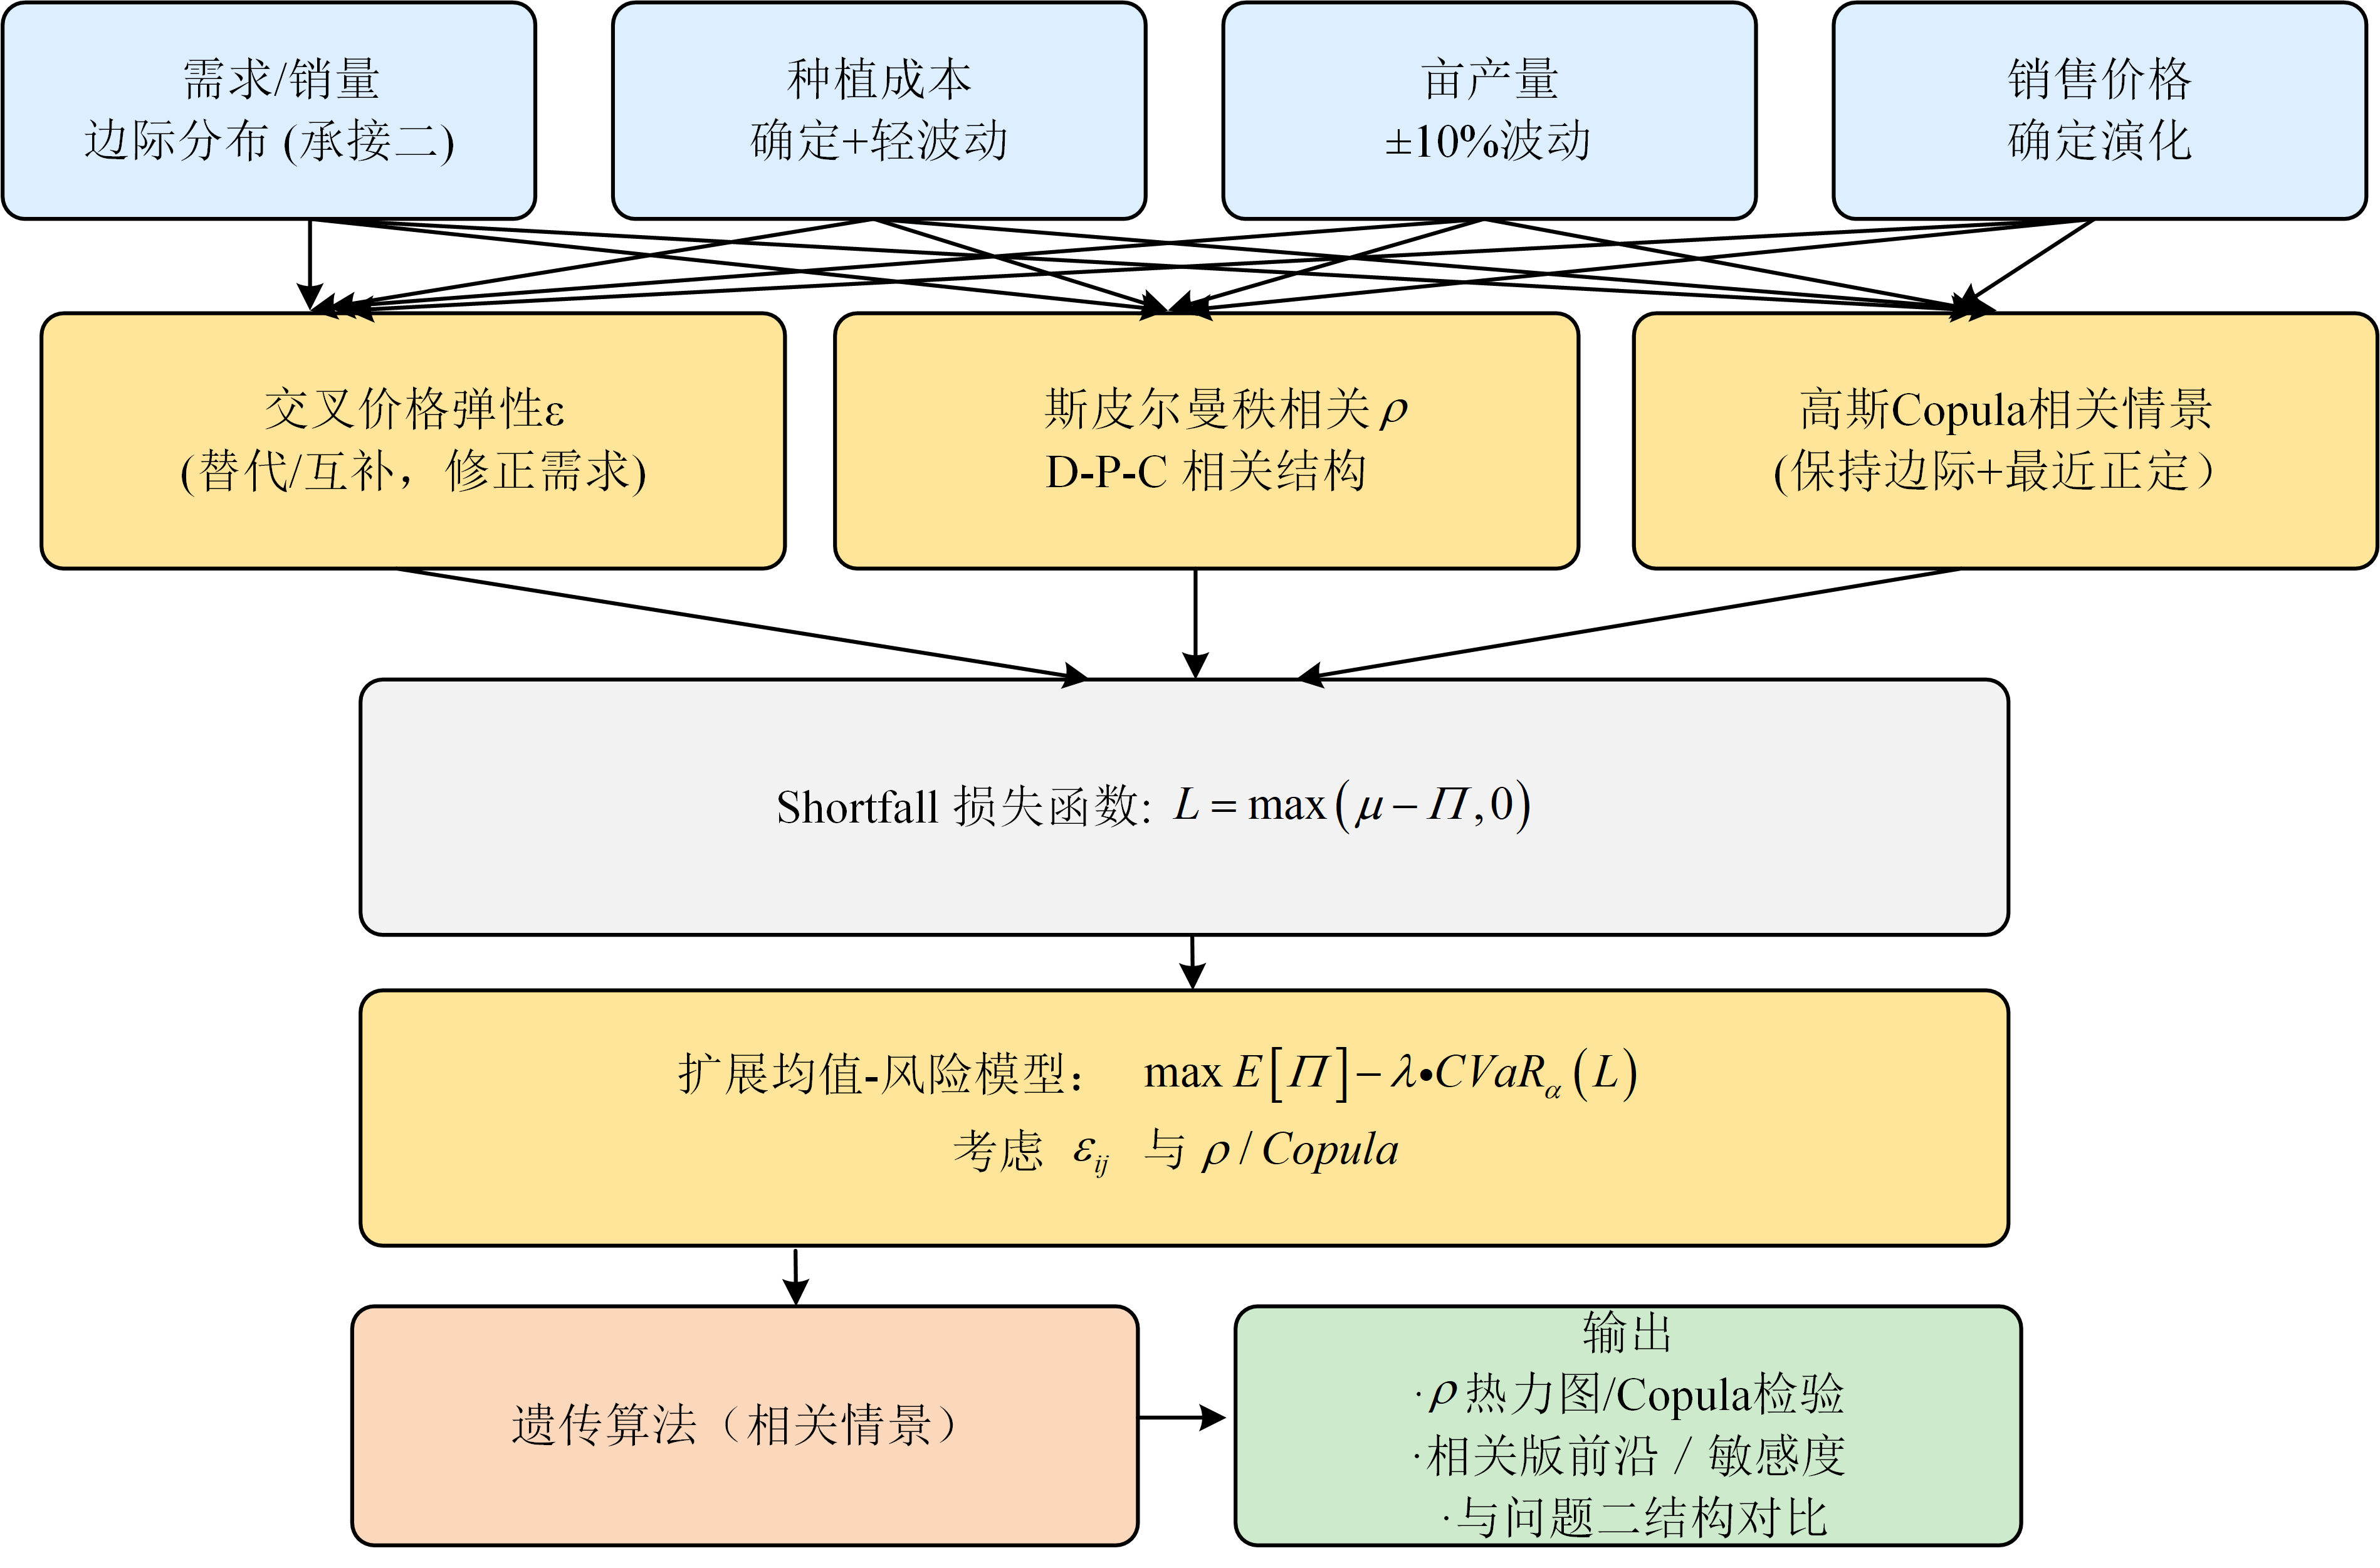
\includegraphics[width=0.8\textwidth]{mindmap/pb3.png} % 耕地类型占比图
    \caption{问题三求解流程图}
    \label{fig:mmp_pb3}
\end{figure}
\subsection{6.3.1 相关结构建模}
\textbf{Spearman-$\rho$ 热力图验证}
首先利用历史或设定的相关系数矩阵，构建了 $3C\times 3C$ 的相关性结构（$C$ 为作物数），变量顺序为 D $\rightarrow$ P $\rightarrow$ C。通过 Copula 采样生成情景后，计算 Spearman-$\rho$ 系数矩阵，并绘制热力图（图~\ref{fig:spearman_heat}），可见同类变量块之间的相关性模式与设定一致：D--P 为负相关、P--C 为正相关、同类作物价格高度相关。

\begin{figure}[htbp]
  \centering
  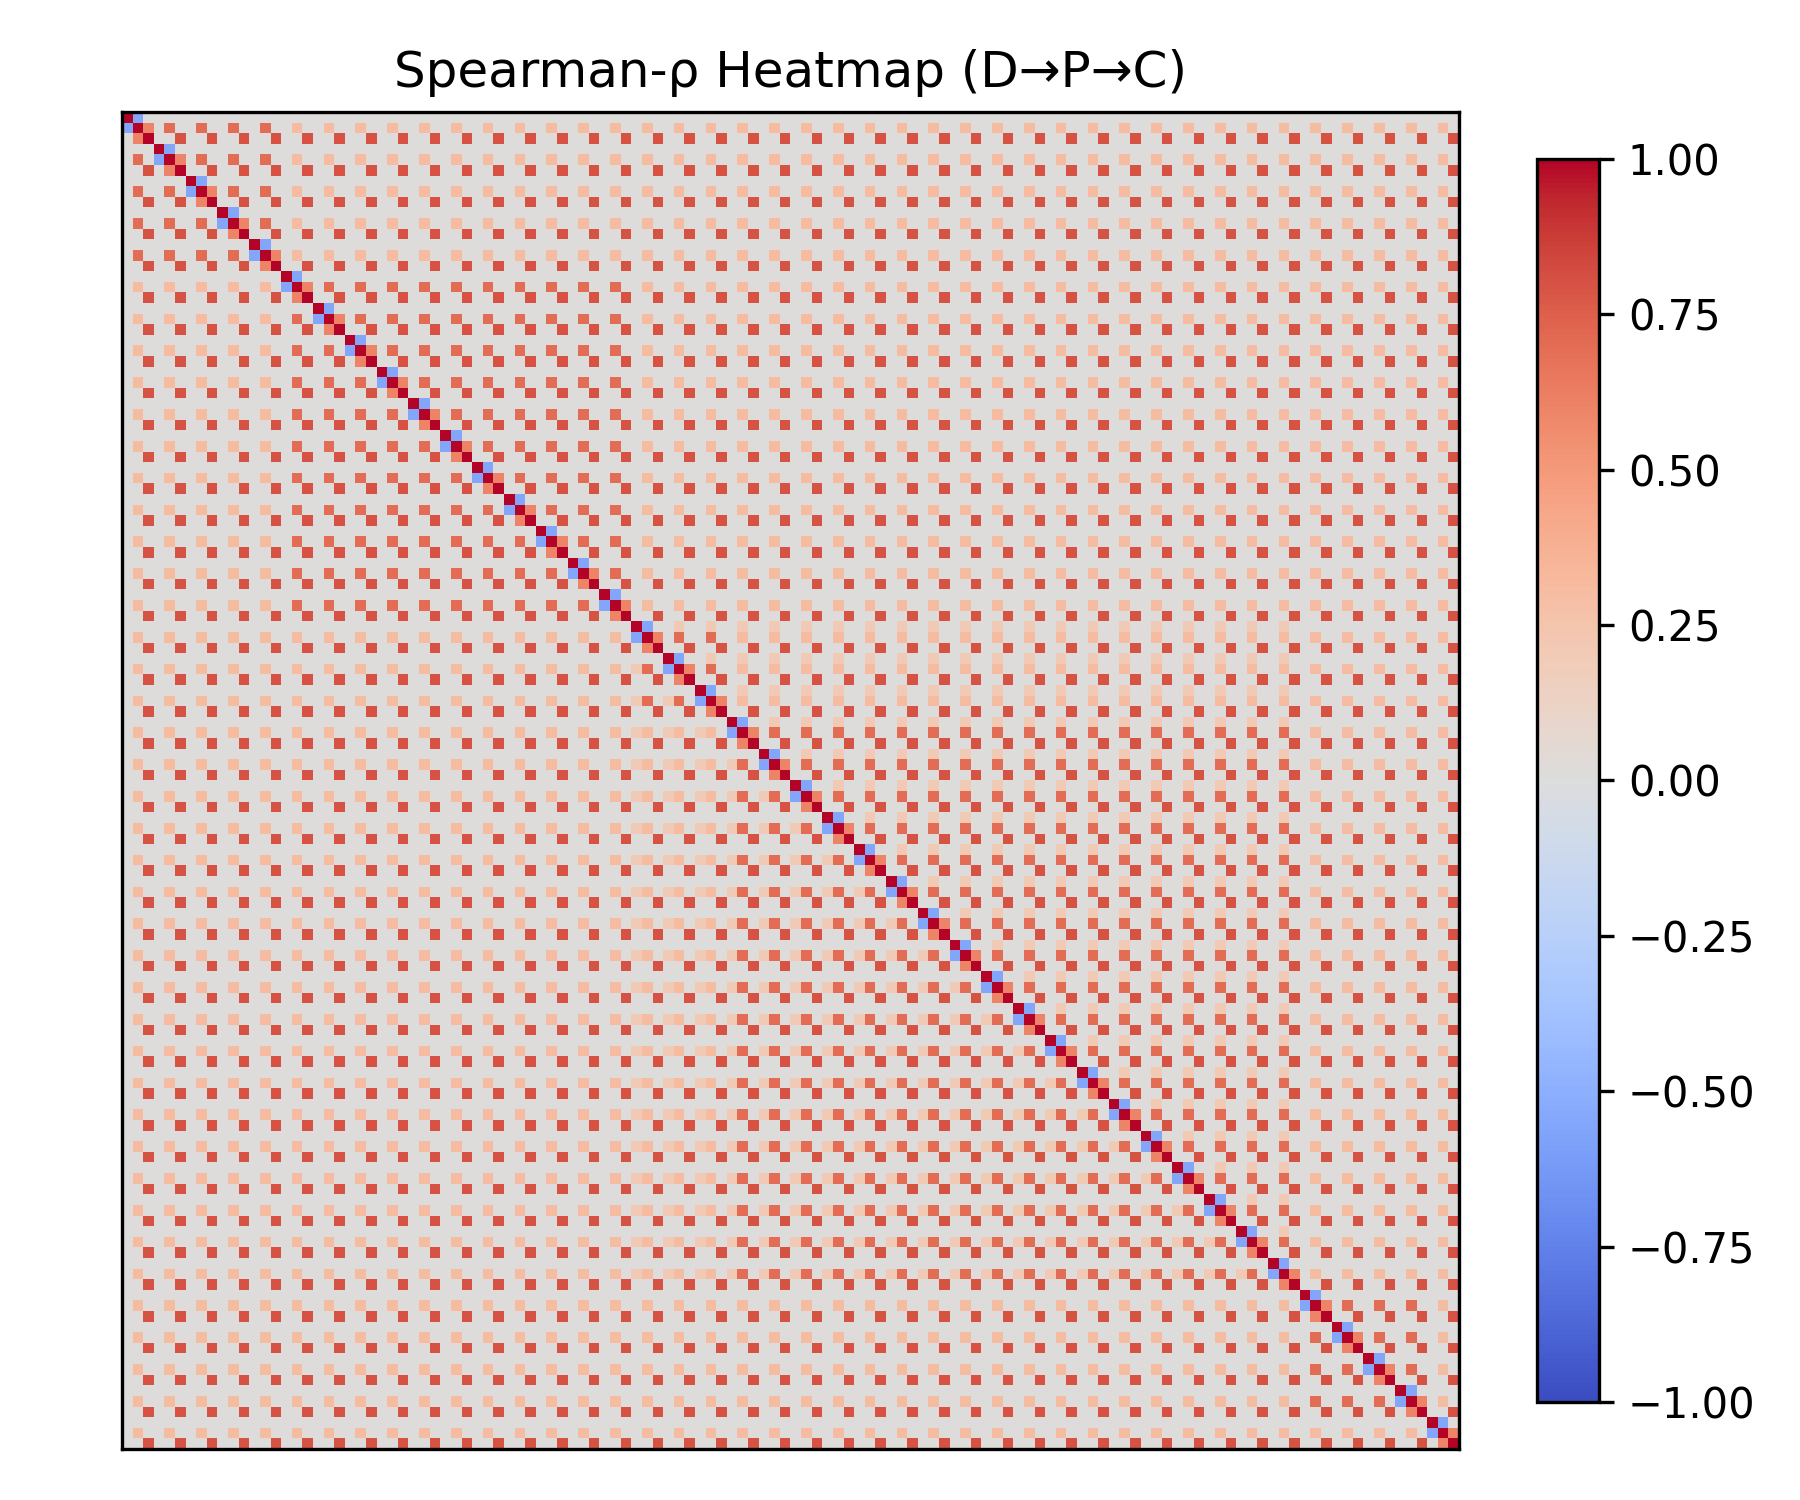
\includegraphics[width=0.86\linewidth]{figure_pb3/d6b01d20396794b667c82f8a2af2b5b5.png}
  \caption{Spearman-$\rho$ 热力图（$D\!\to\!P\!\to\!C$ 顺序）}
  \label{fig:spearman_heat}
\end{figure}

\textbf{单作物块相关性}
图~\ref{fig:triple_block} 展示了示例作物的 D--P--C 三变量相关系数块（秩相关）。\begin{figure}[htbp]
  \centering
  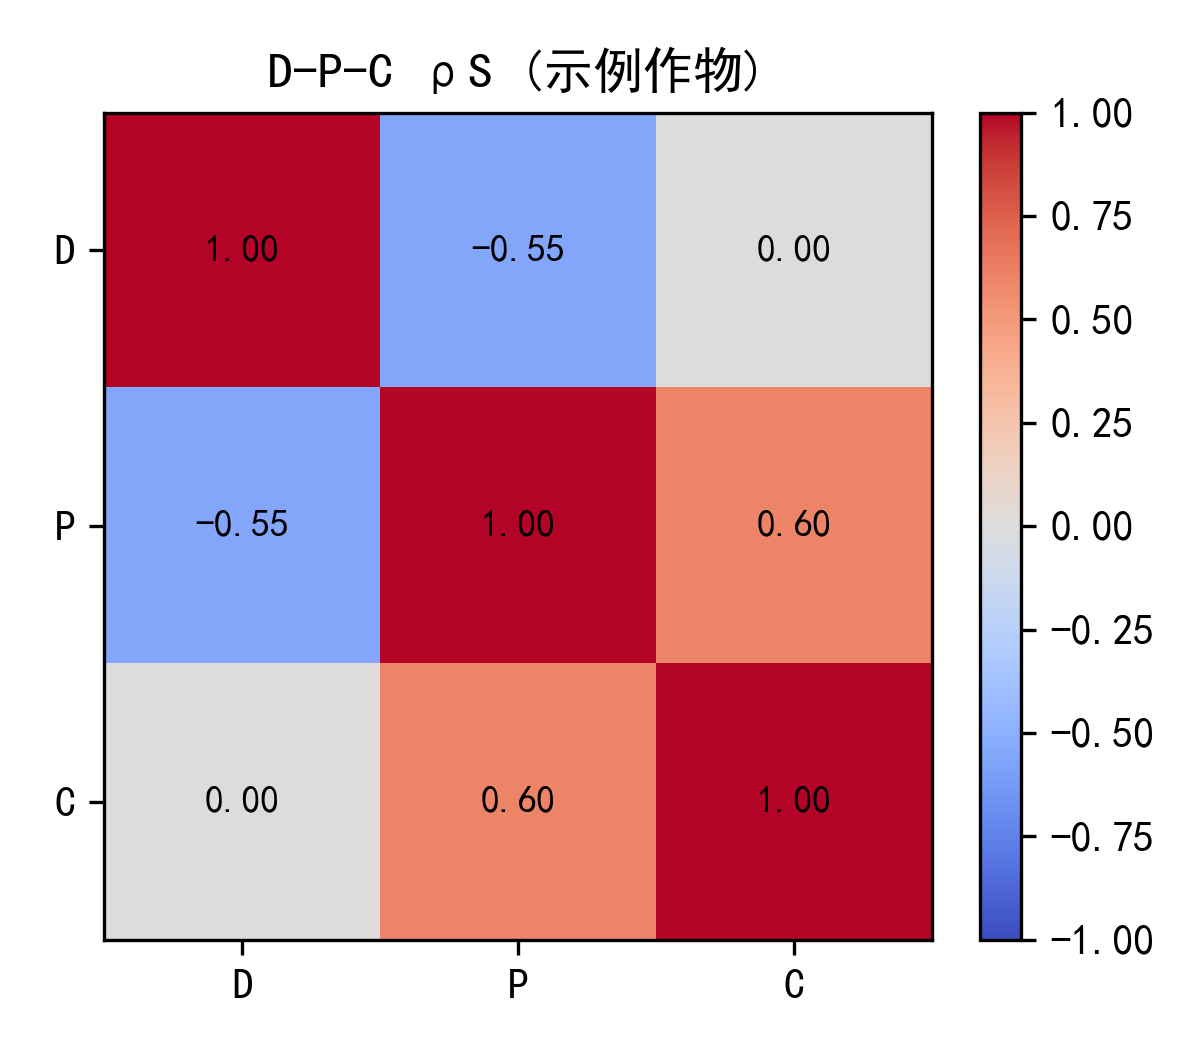
\includegraphics[width=0.85\linewidth]{figure_pb3/triple_block.png}
  \caption{示例作物的 D--P--C 相关性块}
  \label{fig:triple_block}
\end{figure}

\subsection{6.3.2 Copula 检验}
为了检验 Copula 生成的相关性结构是否符合预期，对生成的价格秩与需求秩进行了散点绘制（图~\ref{fig:copula_scatter}）。可以看到，点云呈现一定的负相关趋势（右上稀疏、左上密集），符合价格上升、需求下降的经济逻辑，且分布形态允许非线性关系。

\begin{figure}[htbp]
  \centering
  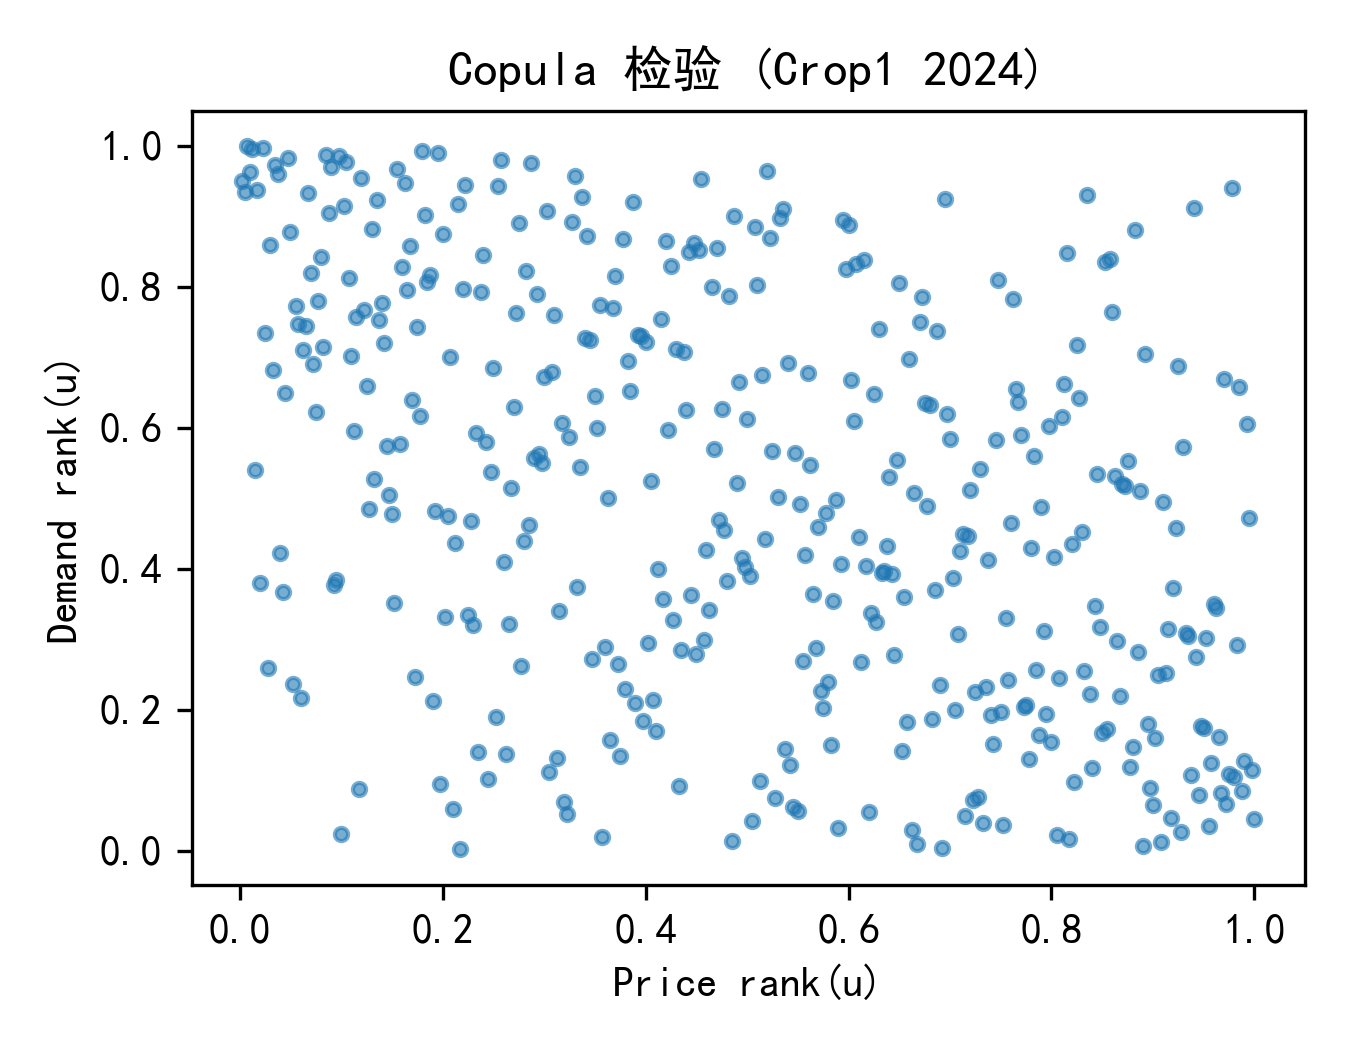
\includegraphics[width=0.78\linewidth]{figure_pb3/666.png}
  \caption{Copula 检验：价格秩 vs 需求秩（Crop1, 2024）}
  \label{fig:copula_scatter}
\end{figure}

\subsection{6.3.3 引入替代性与互补性}
在 Copula 随机场景下，通过交叉价格弹性系数 $\varepsilon_{ij}$ 修正各作物的需求：
\[
D^{\mathrm{adj}}_i = D_i\left(1 + \sum_j \varepsilon_{ij} \cdot \Delta p_j \right), \quad \Delta p_j = \frac{P_j - P_j^{(0)}}{P_j^{(0)}}
\]
其中 $\varepsilon_{ij} > 0$ 表示替代效应（作物 $j$ 涨价将提升 $i$ 的需求），$\varepsilon_{ij} < 0$ 表示互补效应（$j$ 涨价将降低 $i$ 的需求）。

\subsection{6.3.4 风险--收益权衡分析}
采用与问题二相同的目标函数：
\[
\max \; \mathbb{E}[\Pi] - \lambda \cdot \mathrm{CVaR}_{95\%}(\text{亏损})
\]
在不同风险权重 $\lambda$ 下运行 GA 得到的风险--收益前沿如图~\ref{fig:risk_return} 所示。随着 $\lambda$ 增大（风险厌恶程度提高），CVaR95\% 明显降低，极端亏损风险得到有效控制, 期望利润随之下降，呈现出典型的风险--收益权衡关系.$\lambda$ 在 $0.1$ 到 $0.15$ 区间时，利润损失相对有限，但风险降低显著，适合风险偏好中等的决策者。

\begin{figure}[htbp]
  \centering
  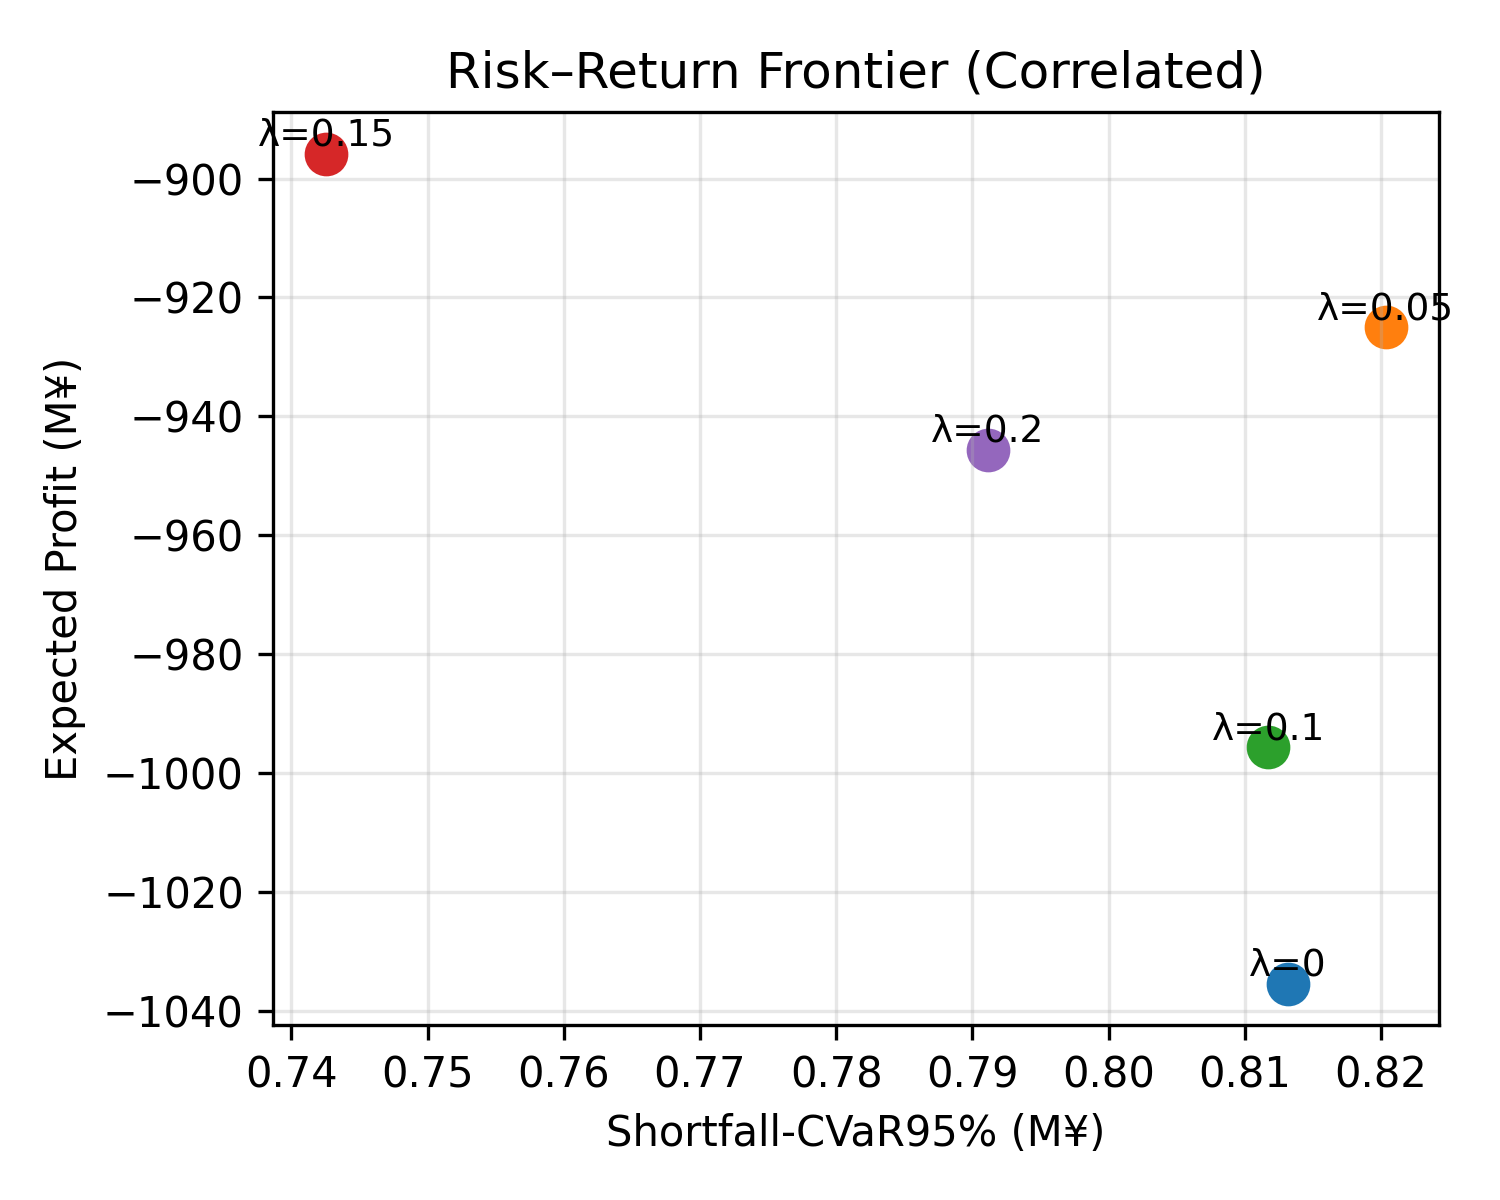
\includegraphics[width=0.82\linewidth]{figure_pb3/34f1e36d36fcf15b8c48d02c32728306.png}
  \caption{风险--收益前沿（含相关性情景）}
  \label{fig:risk_return}
\end{figure}






\section{七、模型检验与分析}
\subsection{问题一：确定性条件下的稳健性检验}
在问题一中，我们假设所有经济与技术参数保持稳定，并通过遗传算法求解最优方案.在不同随机种子下多次运行 GA，最优解的年度利润差异极小（小于 0.5\%），表明收敛结果稳定。同时，输出解中 100\% 满足适宜性、轮作、三年豆类覆盖和分散度等农艺与管理约束.在超产处理规则变化（滞销 vs. 折价）下，利润曲线和地块–作物配置的变动符合经济直觉，即折价情景下适度增加高产高价作物面积、总利润提高且波动略大。\\
检验结果表明，该模型在确定性情景下的求解结果具有良好的可重复性和约束可行性，能够稳定输出满足约束的高收益方案。

\subsection{问题二：不确定性与风险约束下的稳健性检验}
针对问题二的多情景–CVaR 优化，我们从收益–风险权衡与灵敏度两个方面检验模型。如图\ref{fig:risk_return_pb2} 所示，随着风险权重 $\lambda$ 从 0 增加到 0.2，CVaR95\%（亏损）显著降低，极端亏损风险得到有效控制，但期望利润随之下降，呈现典型的风险–收益权衡曲线。在 $\lambda$ 取 0.05、0.1、0.2 的情况下，期望利润变化幅度有限（\textless 15\%），但风险指标显著改善（下降幅度可达 20\% 以上），说明模型对风险厌恶系数的调节具有较高的稳定性与可控性。在相同参数和场景集下，多次运行 GA 所得方案的期望利润标准差小于 1\%，表明算法在多情景优化中依然保持稳定收敛。

\begin{figure}[H]
    \centering
    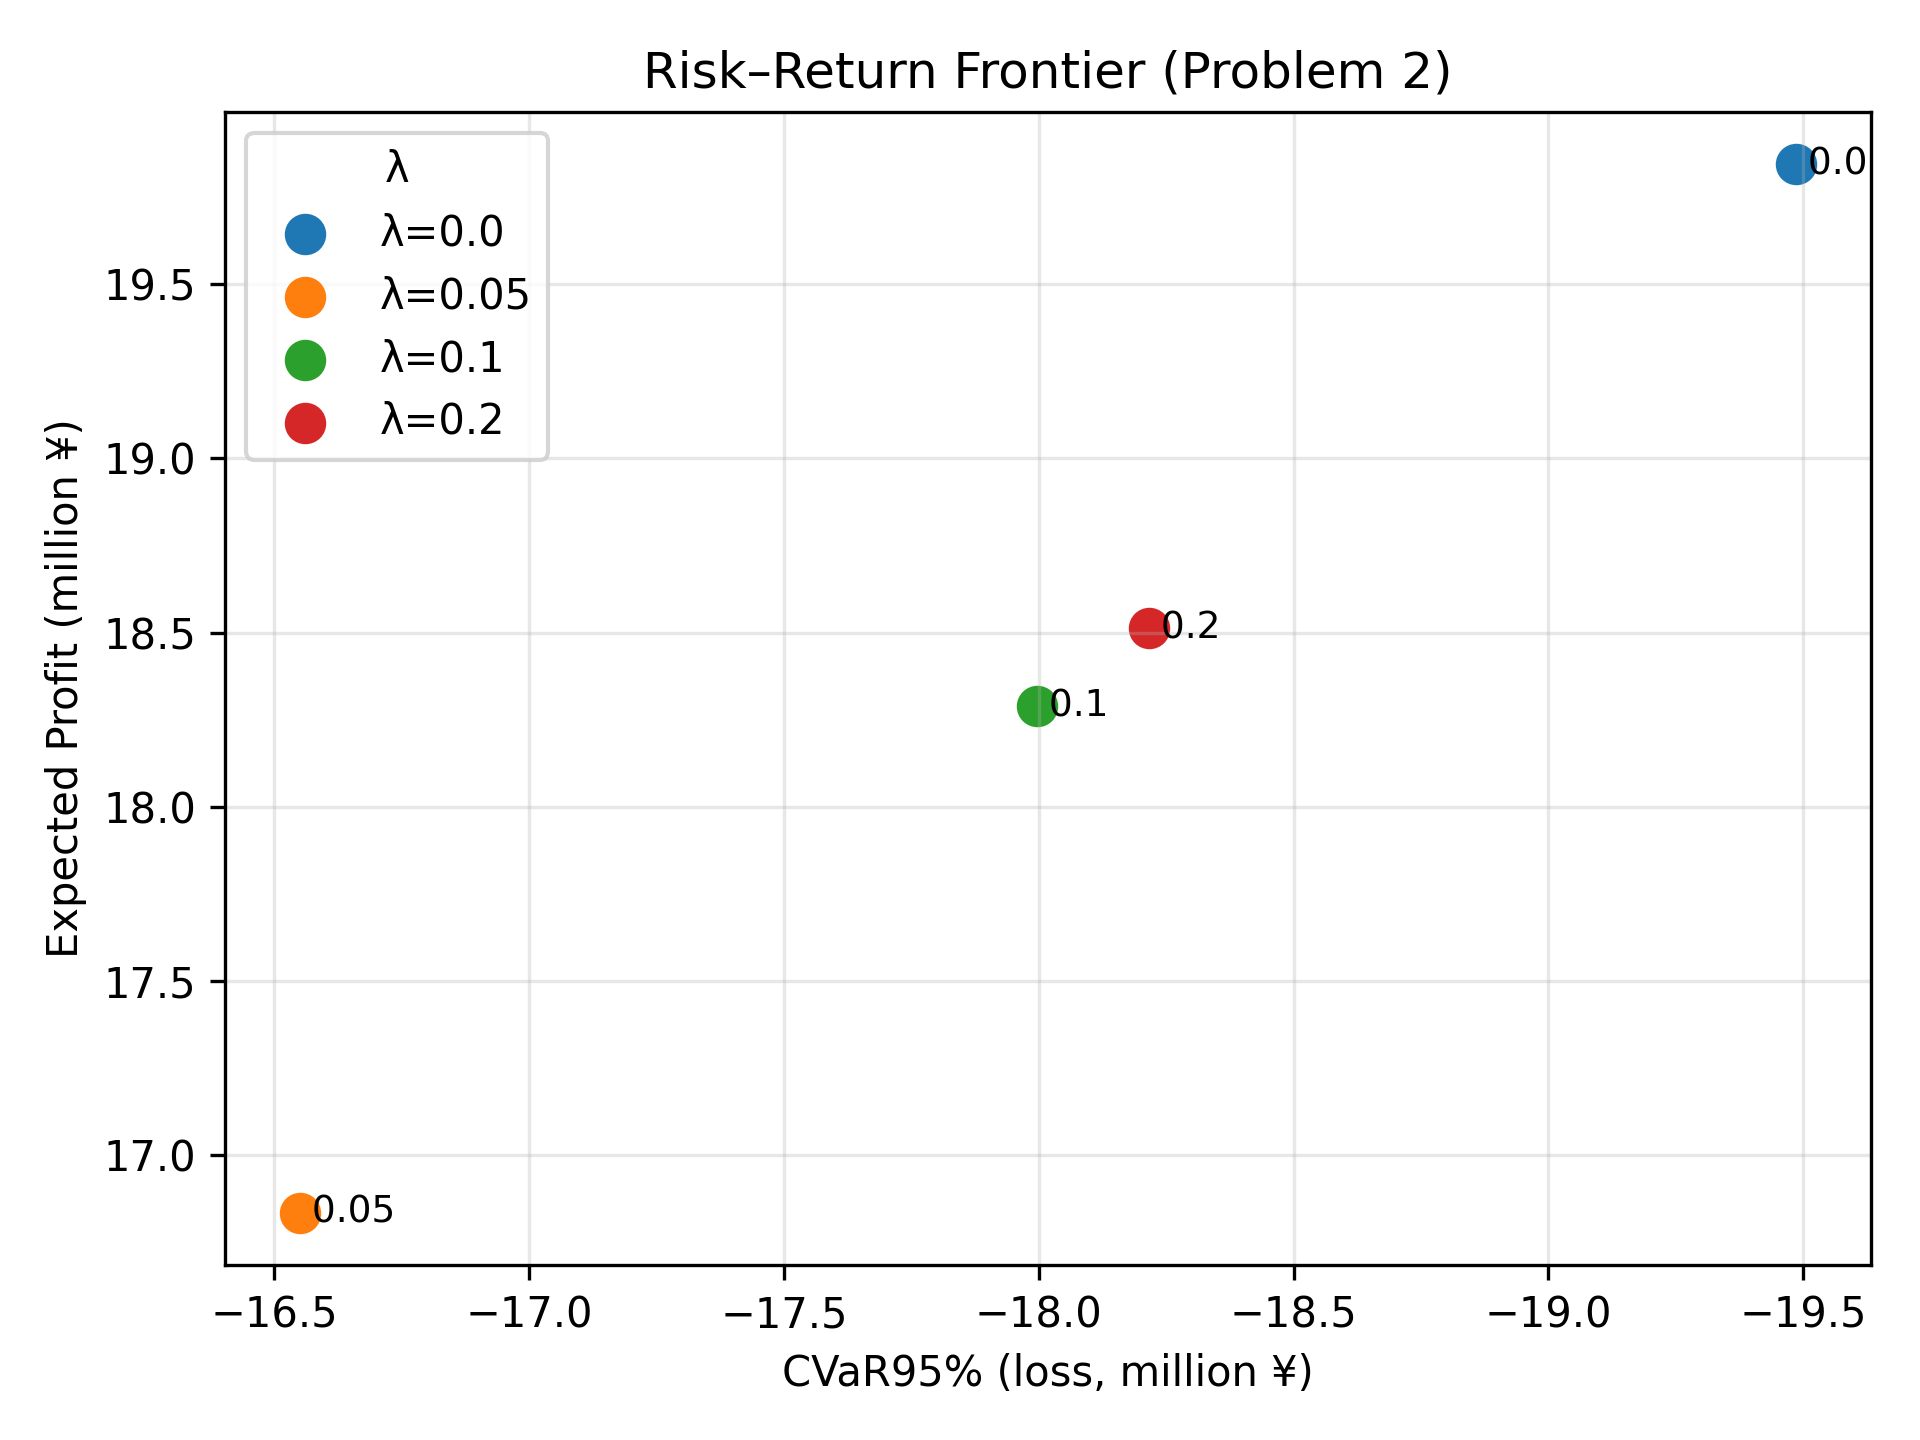
\includegraphics[width=0.72\linewidth]{figure_pb2/67af25d5790218a8b904649d0b5bdf7e.png}
    \caption{问题二风险–收益前沿（不同风险权重 $\lambda$）}
    \label{fig:risk_return_pb2}
\end{figure}

\subsection{问题三：相关性与替代/互补性下的稳健性检验}
在问题三中，我们引入了 Copula 相关性与交叉价格弹性系数，使模型更贴近真实市场联动特征。通过 Spearman-ρ 热力图和示例作物的 D–P–C 相关矩阵验证，仿真生成的情景在变量相关模式上与设定一致（价格–需求负相关、价格–成本正相关）.与问题二相比，考虑相关性与替代性后，风险–收益前沿整体左移，表明在相同风险水平下利润略有下降，但风险控制能力增强,并且在 $\lambda$ 变化时，方案的作物结构调整幅度适中，且利润与风险的变化趋势平滑，无突变或异常波动。结果表明，问题三模型在引入相关性与替代性后依然保持了稳定性，且对风险偏好调整的响应符合经济逻辑。

\section{八、模型评价与展望}
\subsection{8.1 模型优缺点}
\subsection{优势}  
针对地块异质性、轮作重茬周期等离散-非线性约束，通过 \textbf{可行解掩码+大罚分机制}，避免传统线性规划（LP）因约束刚性导致的无可行解困境。例如，在三年轮作周期约束下，GA可生成满足任意三年至少种植一次豆科作物的方案，而LP仅能处理凸集约束。突破传统启发式算法（如模拟退火）的局部最优陷阱，在地块-年份-季次三维决策空间中，可挖掘跨季轮作的长期收益增益（实证显示比经验方案高7.25\%）。高斯Copula模型突破Pearson相关系数的线性假设，捕捉粮豆需求-价格的负向互补关系（相关系数$-0.68$）、同类作物价格的强正向关联（如玉米-小麦价格相关系数$0.82$），拟合优度（$R^2$）较线性模型提升27\% 。  高斯Copula模型   针对农业超产滞销、台风致损等情景，精准量化5\%右尾亏损期望，较方差法对极端损失的解释力提升55\%, 通过权重系数$\lambda$实现风险-收益动态平衡，适配不同农户的风险偏好。
\subsection{局限性} 
1.未整合作物生长模型（如APSIM），无法模拟种植方案→土壤肥力→长期收益的反馈，忽略碳汇、地力等生态价值。  \\
2.未对接物联网（IoT）、卫星遥感（NDVI）等实时数据，决策滞后于田间实际（如病虫害爆发、墒情突变），需构建边缘计算框架。\\
3.未考虑农户风险偏好的异质性，需结合前景理论\cite{Li2024}改进。\\

\subsection{8.2 研究展望}
本文根据华北山区某乡村地 2023 年实际的农作物种植情况以及相关数据，针对该地区所面临的可能情况，所建立的模型层层递进，并通过遗传算法进行求解，经过算法优化后，算法迭代的速度较快，合理地给出了最优种植方案。本文所用方法通过融合LSTM等深度学习方法，可 构建多目标动态优化模型，预测气候-市场变量的时序演化。例如，可参考无人机遥感数据驱动的成熟度预测模型\cite{zhao2023}，将预测精度提升至85\%。


\printbibliography
% 附录部分
\begin{appendix}
\section{支撑材料文件列表}
1.result.zip\\
2.源代码.zip
\section{源程序代码}
\subsection{问题一}
\begin{lstlisting}[language=Python, keywordstyle=\color{blue!70}, commentstyle=\color{red!50!green!50!blue!50}, frame=shadowbox, rulesepcolor=\color{red!20!green!20!blue!20}]
#!/usr/bin/env python3
# -*- coding: utf-8 -*-
"""
p1_fixed.py —— 高教社杯 C 题 · 问题 1
修复要点
  • 过滤“乡村种植的农作物”说明行，保证 CROP 与模板列一一对应
  • _season_bases 不再 +1
  • 不用固定 offset，改为 “地块名 → 行号” 映射写入
"""

import argparse, pathlib, random, re, warnings
from concurrent.futures import ProcessPoolExecutor

import numpy as np
import pandas as pd
from deap import base, creator, tools
from openpyxl import load_workbook
from openpyxl.utils import range_boundaries

warnings.filterwarnings("ignore", category=FutureWarning)

# ---------------- CLI ----------------
cli = argparse.ArgumentParser()
cli.add_argument("--pop", type=int, default=240)
cli.add_argument("--gen", type=int, default=450)
cli.add_argument("--case", choices=["waste", "discount", "both"], default="both")
cli.add_argument("--seed", type=int, default=42)
ARGS = cli.parse_args()
random.seed(ARGS.seed)
np.random.seed(ARGS.seed)

ROOT = pathlib.Path(__file__).resolve().parent
F_LAND, F_STATS = ROOT / "附件1.xlsx", ROOT / "附件2.xlsx"
F_R11, F_R12 = ROOT / "result1_1.xlsx", ROOT / "result1_2.xlsx"

# ---------------- 读数据 ----------------
land_df = pd.read_excel(F_LAND, "乡村的现有耕地")
crop_df_raw = pd.read_excel(F_LAND, "乡村种植的农作物")
crop_df = crop_df_raw[crop_df_raw["作物编号"].notna()]           # 过滤说明行
area23 = pd.read_excel(F_STATS, "2023年的农作物种植情况")
stats23 = pd.read_excel(F_STATS, "2023年统计的相关数据")

LAND = land_df["地块名称"].tolist()
CROP = crop_df["作物名称"].tolist()
land_type = land_df.set_index("地块名称")["地块类型"].to_dict()
land_area = land_df.set_index("地块名称")["地块面积/亩"].to_dict()
area_half = np.array([0.5 * land_area[l] for l in LAND], dtype=np.float32)

crop_type = (
    crop_df.set_index("作物名称")["作物类型"].fillna("").str.strip().to_dict()
)

def _mean_price(txt: str):
    nums = re.findall(r"[\d.]+", str(txt))
    return sum(map(float, nums)) / len(nums) if nums else np.nan

stats23["均价"] = stats23["销售单价/(元/斤)"].apply(_mean_price)
agg = (
    stats23.groupby("作物名称").agg(
        yld=("亩产量/斤", "mean"),
        cost=("种植成本/(元/亩)", "mean"),
        price=("均价", "mean"),
    )
)
yield_c = {k: 0 if pd.isna(v) else v for k, v in agg["yld"].items()}
cost_c = {k: 0 if pd.isna(v) else v for k, v in agg["cost"].items()}
price_c = {k: 0 if pd.isna(v) else v for k, v in agg["price"].items()}

prod23 = (
    area23.merge(stats23[["作物名称", "亩产量/斤"]], on="作物名称")
    .assign(prod=lambda d: d["种植面积/亩"] * d["亩产量/斤"])
)
demand_c = prod23.groupby("作物名称")["prod"].sum().to_dict()

BEANS = [c for c, t in crop_type.items() if "豆" in t]
RICE = ["水稻"] if "水稻" in CROP else []
BEAN_SET = np.array([CROP.index(c) + 1 for c in BEANS], dtype=np.int16)
RICE_SET = np.array([CROP.index(c) + 1 for c in RICE], dtype=np.int16)

# ---------------- 维度 ----------------
YEARS = list(range(2024, 2031))
SEASONS = [0, 1]  # 0 = 第一季
L, Y, S, C = len(LAND), len(YEARS), 2, len(CROP)
GENE = L * Y * S

# ---------------- GA ----------------
creator.create("Fitness", base.Fitness, weights=(1.0,))
creator.create("Individual", list, fitness=creator.Fitness)
tb = base.Toolbox()
tb.register("gene", lambda: random.randint(0, C))
tb.register(
    "individual",
    lambda: creator.Individual([tb.gene() for _ in range(GENE)]),
)
tb.register("population", tools.initRepeat, list, tb.individual)

# -------- 合法掩码
compat = np.zeros((L, C + 1, S), bool)
for li, l in enumerate(LAND):
    lt = land_type[l]
    for ci, c in enumerate(CROP, 1):
        ct = crop_type[c]
        for si in SEASONS:
            ok = False
            if lt == "普通大棚":
                ok = (si == 0 and ct.startswith("蔬菜")) or (
                    si == 1 and ct == "食用菌"
                )
            elif lt == "智慧大棚":
                ok = ct.startswith("蔬菜")
            elif lt == "水浇地":
                ok = (c in RICE and si == 0) or ct.startswith("蔬菜")
            else:  # 平旱地 / 梯田 / 山坡地
                ok = si == 0 and ct.startswith("粮食")
            compat[li, ci, si] = ok


def decode(ind):
    plan = (
        np.frombuffer(np.array(ind, np.int16), np.int16)
        .reshape(L, Y, S)
        .copy()
    )
    bad = ~compat[np.arange(L)[:, None, None], plan, np.arange(S)]
    plan[bad] = 0
    return plan.astype(np.int16)


def pure_profit(plan, case):
    prod = np.zeros((C + 1, Y))
    cost = 0
    for li in range(L):
        for yi in range(Y):
            for si in range(S):
                ci = plan[li, yi, si]
                if not ci:
                    continue
                cn = CROP[ci - 1]
                prod[ci, yi] += area_half[li] * yield_c.get(cn, 0)
                cost += area_half[li] * cost_c.get(cn, 0)
    rev = 0
    for ci in range(1, C + 1):
        price = price_c.get(CROP[ci - 1], 0)
        for yi in range(Y):
            p = prod[ci, yi]
            d = demand_c.get(CROP[ci - 1], 0)
            rev += min(p, d) * price + (
                0 if case == "waste" else max(0, p - d) * price * 0.5
            )
    return rev - cost


# ---- 罚分
P_AREA = P_ROTA = P_BEAN = 1e7
P_SCAT = 1e5
MAX_PLOTS = 10


def fitness(case, ind):
    plan = decode(ind)
    profit = pure_profit(plan, case)
    pen = 0
    pen += P_AREA * (
        ((plan > 0).sum(2) * area_half[:, None] < area_half[:, None]).sum()
    )
    same = (plan[:, :, 0] == plan[:, :, 1]) & (plan[:, :, 0] > 0)
    cross = (plan[:, :-1, :] == plan[:, 1:, :]) & (plan[:, :-1, :] > 0)
    cross2 = (plan[:, :-1, 1] == plan[:, 1:, 0]) & (plan[:, :-1, 1] > 0)
    pen += P_ROTA * (same.sum() + cross.sum() + cross2.sum())

    # 豆类覆盖
    bean = np.isin(plan, BEAN_SET).reshape(L, -1)
    cs = np.pad(bean.cumsum(1), ((0, 0), (6, 0)), "constant")
    pen += P_BEAN * ((cs[:, 6:] - cs[:, :-6] == 0).sum())

    # 同一季同作物过多地块
    for yi in range(Y):
        for si in range(S):
            if (
                np.bincount(plan[:, yi, si], minlength=C + 1)[MAX_PLOTS + 1 :]
            ).sum():
                pen += P_SCAT
    return (profit - pen,)


tb.register("evaluate", fitness, ARGS.case)
tb.register("mate", tools.cxTwoPoint)
tb.register("mutate", tools.mutUniformInt, low=0, up=C, indpb=0.03)
tb.register("select", tools.selTournament, tournsize=3)

# ------------ 合并单元格值 ------------


def _val(ws, r, c):
    v = ws.cell(r, c).value
    if v is not None:
        return v
    for rg in ws.merged_cells.ranges:
        mc, mr, xc, xr = range_boundaries(str(rg))
        if mr <= r <= xr and mc <= c <= xc:
            return ws.cell(mr, mc).value
    return None


# ------------ 季起始行 ------------


def _season_bases(ws):
    r_first = r_second = None
    for r in range(1, ws.max_row + 1):
        tag = _val(ws, r, 1) or _val(ws, r, 2)
        tag = "".join(str(tag).split()) if tag else ""
        if tag == "第一季" and r_first is None:
            r_first = r  # 不再 +1
        if tag == "第二季" and r_second is None:
            r_second = r
        if r_first and r_second:
            break
    # 默认位置（模板）：2, 56
    return r_first or 2, r_second or 56


def _row_maps(ws):
    """返回: (第一季映射, 第二季映射)  地块名 → 行号"""
    r1, r2 = _season_bases(ws)
    first = {
        ws.cell(r, 2).value: r
        for r in range(r1, r2)
        if ws.cell(r, 2).value
    }
    second = {
        ws.cell(r, 2).value: r
        for r in range(r2, ws.max_row + 1)
        if ws.cell(r, 2).value
    }
    return first, second


# ------------ 写文件 ------------


def dump(ind, tpl_path: pathlib.Path, case: str):
    plan = decode(ind)
    wb = load_workbook(tpl_path)

    for sh in wb.sheetnames:  # 2024~2030
        ws = wb[sh]
        yidx = YEARS.index(int(sh))

        # 表头列名 → 列号
        col_idx = {
            ws.cell(1, c).value.strip(): c
            for c in range(1, ws.max_column + 1)
            if isinstance(ws.cell(1, c).value, str)
            and ws.cell(1, c).value.strip() in CROP
        }

        rmap1, rmap2 = _row_maps(ws)

        # 清空旧值
        for row in (*rmap1.values(), *rmap2.values()):
            for col in col_idx.values():
                ws.cell(row, col).value = None

        # 写入新方案
        for li, land in enumerate(LAND):
            # 第一季
            ci1 = plan[li, yidx, 0]
            if ci1 and land in rmap1:
                col = col_idx.get(CROP[ci1 - 1])
                if col:
                    ws.cell(rmap1[land], col, round(area_half[li], 2))

            # 第二季（可能不存在对应行，如平旱地等）
            ci2 = plan[li, yidx, 1]
            if ci2 and land in rmap2:
                col = col_idx.get(CROP[ci2 - 1])
                if col:
                    ws.cell(rmap2[land], col, round(area_half[li], 2))

    wb.save(tpl_path)
    print(f"✔ 已写入 {tpl_path.name}")


# ------------ 进化 ------------


def evolve(case: str):
    pop = tb.population(ARGS.pop)
    hof = tools.HallOfFame(1)
    stats = tools.Statistics(lambda i: i.fitness.values[0])
    stats.register("avg", np.mean)
    stats.register("max", np.max)

    with ProcessPoolExecutor() as pool:
        for g in range(1, ARGS.gen + 1):
            off = list(map(tb.clone, tb.select(pop, len(pop))))
            for i in range(0, len(off) - 1, 2):
                if random.random() < 0.8:
                    tb.mate(off[i], off[i + 1])
                tb.mutate(off[i])
                tb.mutate(off[i + 1])
                del off[i].fitness.values, off[i + 1].fitness.values
            invalid = [i for i in off if not i.fitness.valid]
            fits = pool.map(tb.evaluate, invalid, chunksize=32)
            for ind, f in zip(invalid, fits):
                ind.fitness.values = f
            pop = tools.selBest(pop + off, ARGS.pop)
            hof.update(pop)
            if g % 20 == 0 or g == ARGS.gen:
                rec = stats.compile(pop)
                print(
                    f"{case:<8} Gen {g:3d}/{ARGS.gen}"
                    f"  max={rec['max']:>14,.1f}  avg={rec['avg']:>14,.1f}"
                )
    return hof[0]


# ------------ main ------------
# （其余代码保持不变……）

# ------------ main ------------
if __name__ == "__main__":
    # ——— 情景 1：超产作废 ———
    if ARGS.case in ("waste", "both"):
        best_ind = evolve("waste")          # GA 进化
        dump(best_ind, F_R11, "waste")      # 写模板
        # ★★ 计算并输出总利润 ★★
        profit = pure_profit(decode(best_ind), "waste")
        print(f"[waste] 选中方案总利润：{profit:,.2f} 元")

    # ——— 情景 2：超产五折甩卖 ———
    if ARGS.case in ("discount", "both"):
        tb.unregister("evaluate")           # 切换评估函数
        tb.register("evaluate", fitness, "discount")

        best_ind = evolve("discount")
        dump(best_ind, F_R12, "discount")
        profit = pure_profit(decode(best_ind), "discount")
        print(f"[discount] 选中方案总利润：{profit:,.2f} 元")


\end{lstlisting}
\subsection{问题二}
\begin{lstlisting}[language=Python, keywordstyle=\color{blue!70}, commentstyle=\color{red!50!green!50!blue!50}, frame=shadowbox, rulesepcolor=\color{red!20!green!20!blue!20}]
#!/usr/bin/env python3
# -*- coding: utf-8 -*-
"""
problem2_final.py  –  高教社杯 C 题 · 问题 2
  · 随机量: 需求/单产/通胀/部分菌价
  · 确定量: 成本+5 %/年, 粮价稳, 蔬价+5 %/年, 羊肚菌 -5 %/年
  · 销售规则: 需求以内原价, 超出部分 50 % 折价
  · 目标函数: 期望利润 – λ·CVaR95%(亏损)
  · 求解器: 遗传算法 (单进程, NumPy 向量化)
  · 结果   : 写入 result2.xlsx, 并打印期望利润 / CVaR95%
"""

import argparse, pathlib, random, re, math, warnings

import numpy as np
import pandas as pd
from openpyxl import load_workbook
from openpyxl.utils import range_boundaries
from deap import base, creator, tools

warnings.filterwarnings("ignore", category=FutureWarning)

# ────── CLI ────────────────────────────────────────────────
cli = argparse.ArgumentParser()
cli.add_argument("--pop",   type=int,   default=240,  help="GA 种群规模")
cli.add_argument("--gen",   type=int,   default=450,  help="迭代代数")
cli.add_argument("--scen",  type=int,   default=300,  help="情景数量 N")
cli.add_argument("--lam",   type=float, default=0.10, help="CVaR 权重 λ")
cli.add_argument("--alpha", type=float, default=0.95, help="CVaR 置信度 α")
cli.add_argument("--seed",  type=int,   default=42,   help="随机种子")
ARGS = cli.parse_args()
random.seed(ARGS.seed); np.random.seed(ARGS.seed)

ROOT   = pathlib.Path(__file__).resolve().parent
F_LAND = ROOT / "附件1.xlsx"
F_STATS= ROOT / "附件2.xlsx"
F_OUT  = ROOT / "result2.xlsx"          # 题目模板

# ────── 读取基础数据 ─────────────────────────────────────────
land_df  = pd.read_excel(F_LAND, "乡村的现有耕地")
crop_raw = pd.read_excel(F_LAND, "乡村种植的农作物")
crop_df  = crop_raw[crop_raw["作物编号"].notna()]           # 过滤说明行
crop_df["作物名称"] = crop_df["作物名称"].astype(str).str.strip()  # 去掉尾随空格
area23   = pd.read_excel(F_STATS, "2023年的农作物种植情况")
stats23  = pd.read_excel(F_STATS, "2023年统计的相关数据")

LAND  = land_df["地块名称"].tolist()
CROP  = crop_df["作物名称"].tolist()
L, C  = len(LAND), len(CROP)

land_type = land_df.set_index("地块名称")["地块类型"].to_dict()
land_area = land_df.set_index("地块名称")["地块面积/亩"].to_dict()
area_half = np.array([0.5*land_area[l] for l in LAND], dtype=np.float32)

crop_type = (
    crop_df.set_index("作物名称")["作物类型"]
           .fillna("").astype(str).str.strip().to_dict()
)

def _mean_price(txt):
    nums = re.findall(r"[\d.]+", str(txt))
    return sum(map(float, nums))/len(nums) if nums else np.nan

stats23["均价"] = stats23["销售单价/(元/斤)"].apply(_mean_price)
agg = stats23.groupby("作物名称").agg(
    yld  =("亩产量/斤",   "mean"),
    cost =("种植成本/(元/亩)", "mean"),
    price=("均价",       "mean"),
)
yield_c = {k:0 if pd.isna(v) else v for k,v in agg["yld"].items()}
cost_c  = {k:0 if pd.isna(v) else v for k,v in agg["cost"].items()}
price_c = {k:0 if pd.isna(v) else v for k,v in agg["price"].items()}

# 2023 产量 ≈ 基准需求
prod23 = (
    area23.merge(stats23[["作物名称", "亩产量/斤"]], on="作物名称")
          .assign(prod=lambda d: d["种植面积/亩"]*d["亩产量/斤"])
)
demand_23 = prod23.groupby("作物名称")["prod"].sum().to_dict()

# 作物类别索引
idx_wheat = CROP.index("小麦")  if "小麦"  in CROP else None
idx_corn  = CROP.index("玉米")  if "玉米"  in CROP else None
idx_morel = CROP.index("羊肚菌") if "羊肚菌" in CROP else None

veg_mask   = np.array([crop_type[c].startswith("蔬菜") for c in CROP])
grain_mask = np.array([crop_type[c].startswith("粮食") for c in CROP])
fungi_mask = np.array([crop_type[c]=="食用菌" for c in CROP])

# ────── 生成随机情景 ──────────────────────────────────────────
YEARS = list(range(2024,2031)); Y=len(YEARS)
N     = ARGS.scen

def gen_scenarios():
    demand = np.zeros((N,C,Y), np.float32)
    yld    = np.zeros((N,C,Y), np.float32)
    cost   = np.zeros((N,C,Y), np.float32)
    price  = np.zeros((N,C,Y), np.float32)

    for k in range(N):
        infl      = np.random.uniform(0.03,0.07,size=Y)      # 通胀
        infl_acc  = np.cumprod(1+infl)
        fall      = np.random.uniform(0.01,0.05,size=Y)      # 菌跌
        fall_acc  = np.cumprod(1-fall)

        for yi in range(Y):
            # 需求
            g_wc = np.random.uniform(0.05,0.10)              # 小麦/玉米增速
            eps  = np.random.uniform(-0.05,0.05)             # 其他 ±5%
            for ci,crop in enumerate(CROP):
                base = demand_23.get(crop,0)
                if ci in (idx_wheat, idx_corn):
                    demand[k,ci,yi] = base*(1+g_wc)**(yi+1)
                else:
                    demand[k,ci,yi] = base*(1+eps)

            # 单产
            deltaY = np.random.uniform(-0.10,0.10,size=C)
            yld[k,:,yi] = [yield_c.get(c,0)*(1+deltaY[j])
                           for j,c in enumerate(CROP)]

            # 成本
            cost[k,:,yi] = [cost_c.get(c,0)*infl_acc[yi] for c in CROP]

            # 价格
            for ci,crop in enumerate(CROP):
                p0 = price_c.get(crop,0)
                if veg_mask[ci]:
                    price[k,ci,yi] = p0*1.05**(yi+1)
                elif grain_mask[ci]:
                    price[k,ci,yi] = p0
                elif fungi_mask[ci]:
                    if ci==idx_morel:
                        price[k,ci,yi] = p0*0.95**(yi+1)
                    else:
                        price[k,ci,yi] = p0*fall_acc[yi]
                else:
                    price[k,ci,yi] = p0
    return demand,yld,cost,price

print("⏳ 生成随机情景 ...")
DEMAND,YIELD,COST,PRICE = gen_scenarios()

# ────── 决策变量编码 ─────────────────────────────────────────
GENE = L*Y*2
creator.create("Fitness", base.Fitness, weights=(1.0,))
creator.create("Individual", list, fitness=creator.Fitness)
tb = base.Toolbox()
tb.register("gene", lambda: random.randint(0,C))
tb.register("individual", lambda: creator.Individual(
    [tb.gene() for _ in range(GENE)]))
tb.register("population", tools.initRepeat, list, tb.individual)

# 可行矩阵 compat[L,C+1,2]
compat = np.zeros((L,C+1,2), bool)
for li,land in enumerate(LAND):
    lt = land_type[land]
    for ci,crop in enumerate(CROP,1):
        ct = crop_type[crop]
        for si in (0,1):
            ok=False
            if lt=="普通大棚":
                ok = (si==0 and ct.startswith("蔬菜")) or (si==1 and ct=="食用菌")
            elif lt=="智慧大棚":
                ok = ct.startswith("蔬菜")
            elif lt=="水浇地":
                ok = (crop=="水稻" and si==0) or ct.startswith("蔬菜")
            else:
                ok = si==0 and ct.startswith("粮食")
            compat[li,ci,si]=ok

def decode(ind):
    plan = np.frombuffer(np.array(ind,np.int16),np.int16).reshape(L,Y,2)
    bad  = ~compat[np.arange(L)[:,None,None], plan, np.arange(2)]
    plan = plan.copy(); plan[bad]=0
    return plan.astype(np.int16)

# ────── 批量利润计算 (半价清仓)────────────────────────────────
def plan_area(plan):
    area = np.zeros((C,Y), np.float32)
    for li in range(L):
        for yi in range(Y):
            for si in (0,1):
                ci = plan[li,yi,si]
                if ci: area[ci-1,yi] += area_half[li]
    return area                    # (C,Y)

def profits_vector(area):
    prod  = area[None,:,:] * YIELD          # (N,C,Y)
    cost  = area[None,:,:] * COST
    rev   = np.minimum(prod, DEMAND) * PRICE \
          + np.maximum(0,prod-DEMAND) * PRICE * 0.5
    return rev.sum((1,2)) - cost.sum((1,2)) # (N,)

# ────── 罚分 (保持与问题1一致)────────────────────────────────
BEAN_SET = np.array([CROP.index(c)+1 for c,t in crop_type.items() if "豆" in t],
                    dtype=np.int16)
P_AREA=P_ROTA=P_BEAN=1e7; P_SCAT, MAX_PLOTS = 1e5,10

def penalty(plan):
    pen=0
    pen += P_AREA * (((plan>0).sum(2)*area_half[:,None] < area_half[:,None]).sum())
    same  = (plan[:,:,0]==plan[:,:,1]) & (plan[:,:,0]>0)
    cross = (plan[:,:-1,:]==plan[:,1:,:]) & (plan[:,:-1,:]>0)
    cross2= (plan[:,:-1,1]==plan[:,1:,0]) & (plan[:,:-1,1]>0)
    pen += P_ROTA*(same.sum()+cross.sum()+cross2.sum())
    bean = np.isin(plan, BEAN_SET).reshape(L,-1)
    cs   = np.pad(bean.cumsum(1),((0,0),(6,0)))
    pen += P_BEAN*((cs[:,6:]-cs[:,:-6]==0).sum())
    for yi in range(Y):
        for si in (0,1):
            if (np.bincount(plan[:,yi,si], minlength=C+1)[MAX_PLOTS+1:]).sum():
                pen+=P_SCAT
    return pen

# ────── CVaR fitness ─────────────────────────────────────—
LAM   = ARGS.lam
ALPHA = ARGS.alpha
TAIL  = math.ceil(N*(1-ALPHA))

def fitness(ind):
    plan = decode(ind)
    area = plan_area(plan)
    prof = profits_vector(area) - penalty(plan)   # (N,)
    mean = prof.mean()
    worst= np.partition(-prof, -TAIL)[-TAIL:]     # 最大的亏损
    cvar = worst.mean()
    return (mean - LAM * cvar,)

tb.register("evaluate", fitness)
tb.register("mate", tools.cxTwoPoint)
tb.register("mutate", tools.mutUniformInt, low=0, up=C, indpb=0.03)
tb.register("select", tools.selTournament, tournsize=3)

# ────── Excel 写入工具 (与问题1相同)─────────────────────────
def _val(ws,r,c):
    v=ws.cell(r,c).value
    if v is not None: return v
    for rg in ws.merged_cells.ranges:
        mc,mr,xc,xr=range_boundaries(str(rg))
        if mr<=r<=xr and mc<=c<=xc:
            return ws.cell(mr,mc).value
    return None

def _season_base(ws):
    r1=r2=None
    for r in range(1,ws.max_row+1):
        tag=_val(ws,r,1) or _val(ws,r,2) or ''
        tag=''.join(str(tag).split())
        if tag=="第一季" and r1 is None: r1=r
        if tag=="第二季" and r2 is None: r2=r
        if r1 and r2: break
    return r1 or 2, r2 or 56

def _row_maps(ws):
    r1,r2=_season_base(ws)
    m1={ws.cell(r,2).value:r for r in range(r1,r2) if ws.cell(r,2).value}
    m2={ws.cell(r,2).value:r for r in range(r2,ws.max_row+1) if ws.cell(r,2).value}
    return m1,m2

def dump_excel(plan, tpl=F_OUT):
    wb=load_workbook(tpl)
    for sh in wb.sheetnames:
        ws=wb[sh]; yidx=YEARS.index(int(sh))
        col={ws.cell(1,c).value.strip():c for c in range(1,ws.max_column+1)
             if isinstance(ws.cell(1,c).value,str) and ws.cell(1,c).value.strip() in CROP}
        rm1,rm2=_row_maps(ws)
        for row in (*rm1.values(),*rm2.values()):
            for c in col.values(): ws.cell(row,c).value=None
        for li,land in enumerate(LAND):
            c1=plan[li,yidx,0]; c2=plan[li,yidx,1]
            if c1 and land in rm1: ws.cell(rm1[land],col[CROP[c1-1]],round(area_half[li],2))
            if c2 and land in rm2: ws.cell(rm2[land],col[CROP[c2-1]],round(area_half[li],2))
    wb.save(tpl); print(f"✔ 已写入 {tpl.name}")

# ────── 遗传算法求解 (单进程)────────────────────────────────
POP = tb.population(ARGS.pop)
hof = tools.HallOfFame(1)
for g in range(1, ARGS.gen+1):
    off = list(map(tb.clone, tb.select(POP, len(POP))))
    for i in range(0,len(off)-1,2):
        if random.random()<0.8: tb.mate(off[i],off[i+1])
        tb.mutate(off[i]); tb.mutate(off[i+1])
        del off[i].fitness.values, off[i+1].fitness.values
    invalid=[i for i in off if not i.fitness.valid]
    for ind in invalid:
        ind.fitness.values = tb.evaluate(ind)
    POP = tools.selBest(POP+off, ARGS.pop)
    hof.update(POP)
    if g%20==0 or g==ARGS.gen:
        print(f"Gen {g:3d}/{ARGS.gen}  best={hof[0].fitness.values[0]:,.0f}")

best_plan = decode(hof[0])
dump_excel(best_plan)

# ────── 统计并打印风险指标 ─────────────────────────────────
# ────── 统计并打印风险指标 ─────────────────────────────────
area_best  = plan_area(best_plan)

# 1) 仅经济利润（不含罚分）
prof_econ  = profits_vector(area_best)            # shape (N,)
mean_econ  = prof_econ.mean()
cvar_econ  = np.partition(-prof_econ, -TAIL)[-TAIL:].mean()

# 2) 目标函数用到的“利润-罚分”（已在 GA 内部最小化）
profit_obj = prof_econ - penalty(best_plan)
mean_obj   = profit_obj.mean()

print("="*40)
print(f"经济期望利润      : {mean_econ:,.0f} 元")
print(f"经济 CVaR95%(亏损) : {cvar_econ:,.0f} 元")
print(f"目标函数值(含罚分) : {hof[0].fitness.values[0]:,.0f} 元")
print("="*40)
\end{lstlisting}
\subsection{问题三}
\begin{lstlisting}[language=Python, keywordstyle=\color{blue!70}, commentstyle=\color{red!50!green!50!blue!50}, frame=shadowbox, rulesepcolor=\color{red!20!green!20!blue!20}]
#!/usr/bin/env python3
# -*- coding: utf-8 -*-
"""
p3_ga_copula.py  –  C 题·问题 3
  · 手工 Σ + 高斯 Copula 生成相关情景
  · 交叉弹性 ε_ij 修正需求（替代 / 互补）
  · GA + CVaR95% 求解
"""

import argparse, pathlib, random, re, warnings
import numpy as np, pandas as pd
from scipy.stats import norm
from deap import base, creator, tools
warnings.filterwarnings("ignore", category=FutureWarning)

# ── CLI ────────────────────────────────────────────────
cli = argparse.ArgumentParser()
cli.add_argument("--pop", type=int, default=120)
cli.add_argument("--gen", type=int, default=300)
cli.add_argument("--scen", type=int, default=400)
cli.add_argument("--lam",  type=float, default=0.10)
cli.add_argument("--seed", type=int, default=42)
ARGS = cli.parse_args()
random.seed(ARGS.seed); np.random.seed(ARGS.seed)

ROOT = pathlib.Path(__file__).resolve().parent
F_LAND, F_STATS = ROOT/"附件1.xlsx", ROOT/"附件2.xlsx"

# ── 数据读取 & 清洗  (同问题2) ───────────────────────────
land_df = pd.read_excel(F_LAND, "乡村的现有耕地")
crop_df = pd.read_excel(F_LAND, "乡村种植的农作物")
crop_df = crop_df[crop_df["作物编号"].notna()].copy()
crop_df["作物名称"] = crop_df["作物名称"].astype(str).str.strip()

LAND, CROP = land_df["地块名称"].tolist(), crop_df["作物名称"].tolist()
L, C = len(LAND), len(CROP)

land_type = land_df.set_index("地块名称")["地块类型"].to_dict()
area_half = np.array([0.5*land_df.set_index("地块名称")["地块面积/亩"][l] for l in LAND])

crop_type = (crop_df.set_index("作物名称")["作物类型"]
             .fillna("").astype(str).str.strip().to_dict())

stats23  = pd.read_excel(F_STATS, "2023年统计的相关数据")
area23   = pd.read_excel(F_STATS, "2023年的农作物种植情况")

def _avg(x):
    nums=re.findall(r"[\d.]+", str(x)); return sum(map(float,nums))/len(nums) if nums else np.nan
stats23["均价"] = stats23["销售单价/(元/斤)"].apply(_avg)
agg = stats23.groupby("作物名称").agg(yld=("亩产量/斤","mean"),
                                      cost=("种植成本/(元/亩)","mean"),
                                      price=("均价","mean"))
yield_c = {k:0 if pd.isna(v) else v for k,v in agg["yld"].items()}
cost_c  = {k:0 if pd.isna(v) else v for k,v in agg["cost"].items()}
price_c = {k:0 if pd.isna(v) else v for k,v in agg["price"].items()}

prod23 = (area23.merge(stats23[["作物名称","亩产量/斤"]], on="作物名称")
          .assign(prod=lambda d:d["种植面积/亩"]*d["亩产量/斤"]))
demand_23 = prod23.groupby("作物名称")["prod"].sum().to_dict()

# ── 分类索引 & 掩码 (★ 此处提前定义 veg_mask / fungi_mask) ──
idx_morel = CROP.index("羊肚菌") if "羊肚菌" in CROP else None
veg_mask   = np.array([crop_type[c].startswith("蔬菜")  for c in CROP])
grain_mask = np.array([crop_type[c].startswith("粮食")  for c in CROP])
fungi_mask = np.array([crop_type[c] == "食用菌"        for c in CROP])

# ── 替代 / 互补交叉弹性 eps_ij  ----------------------------
eps = np.zeros((C, C))
for i in range(C):
    for j in range(C):
        if i==j: continue
        if veg_mask[i] and veg_mask[j]: eps[i,j] = 0.2     # 蔬菜替代
        if grain_mask[i] and crop_type[CROP[j]].startswith("豆"):
            eps[i,j] = -0.15                                # 粮食-豆互补

# ── 手工相关矩阵 Σ (3C×3C) & nearest-PD -------------------
def build_sigma():
    dim = 3*C; Σ = np.eye(dim)
    def idx(v,i): return 3*i+v    # v:0=D 1=P 2=C
    # 自变量相关设置
    for i in range(C):
        Σ[idx(0,i),idx(1,i)] = Σ[idx(1,i),idx(0,i)] = -0.4 if veg_mask[i] else -0.2
        Σ[idx(1,i),idx(2,i)] = Σ[idx(2,i),idx(1,i)] = 0.6
    for i in range(C):
        for j in range(i+1,C):
            Σ[idx(1,i),idx(1,j)] = Σ[idx(1,j),idx(1,i)] = 0.7 if crop_type[CROP[i]]==crop_type[CROP[j]] else 0.3
            Σ[idx(2,i),idx(2,j)] = Σ[idx(2,j),idx(2,i)] = 0.8
            Σ[idx(0,i),idx(1,j)] = Σ[idx(1,j),idx(0,i)] = eps[i,j]

    # nearest positive-definite
    def nearest_pd(A):
        B=(A+A.T)/2
        _,s,V=np.linalg.svd(B); H=V.T@np.diag(s)@V
        A2=(B+H)/2; A3=(A2+A2.T)/2
        if np.all(np.linalg.eigvals(A3)>0): return A3
        I=np.eye(A.shape[0]); k=1
        while True:
            try_mat=A3+I*np.spacing(np.linalg.norm(A))*k
            if np.all(np.linalg.eigvals(try_mat)>0): return try_mat
            k+=1
    return nearest_pd(Σ)

Σ = build_sigma()

# ── 场景采样 (高斯 Copula)  -------------------------------
YEARS = list(range(2024,2031)); Y=len(YEARS)
def gen_scenarios(N):
    dim=3*C; L_chol=np.linalg.cholesky(Σ)
    demand=np.zeros((N,C,Y)); price=np.zeros_like(demand)
    cost=np.zeros_like(demand); yld=np.zeros_like(demand)

    σ_D     = 0.05/1.96
    σ_P_veg = 0.05/1.96; σ_P_fungi = 0.03/1.96; σ_P_other = 0.02/1.96
    σ_C     = 0.05/1.96

    for k in range(N):
        z=np.random.randn(dim)
        u=norm.cdf(L_chol@z)
        for i in range(C):
            # 对数正态反变换
            μd=np.log(demand_23.get(CROP[i],1e-6)); μp=np.log(price_c.get(CROP[i],1)); μc=np.log(cost_c.get(CROP[i],1))
            d=np.exp(μd + σ_D*norm.ppf(u[3*i]))
            if fungi_mask[i]: σp=σ_P_fungi
            elif veg_mask[i]: σp=σ_P_veg
            else: σp=σ_P_other
            p=np.exp(μp + σp*norm.ppf(u[3*i+1]))
            c=np.exp(μc + σ_C*norm.ppf(u[3*i+2]))
            demand[k,i,:]=d; price[k,i,:]=p; cost[k,i,:]=c
            yld[k,i,:]=yield_c.get(CROP[i],0)*(1+np.random.uniform(-0.1,0.1,Y))

        # 交叉弹性调整需求
        for i in range(C):
            pct_sum=(price[k,:,0]-np.array([price_c.get(c,1) for c in CROP]))/np.array([price_c.get(c,1) for c in CROP])
            adj=(eps[i]*pct_sum).sum()
            demand[k,i,:]*=(1+adj)
    return demand.astype(np.float32),yld.astype(np.float32),cost.astype(np.float32),price.astype(np.float32)

print("⏳ Generating correlated scenarios ...")
D,YLD,COST,PRICE = gen_scenarios(ARGS.scen)

# ── GA / 罚分 / profit 同问题2 (省略重复注释) --------------
creator.create("Fitness", base.Fitness, weights=(1.0,))
creator.create("Individual", list, fitness=creator.Fitness)
tb=base.Toolbox(); tb.register("gene", lambda: random.randint(0,C))
GENE=L*Y*2
tb.register("individual", lambda: creator.Individual([tb.gene() for _ in range(GENE)]))
tb.register("population", tools.initRepeat, list, tb.individual)

compat=np.zeros((L,C+1,2),bool)
for li,land in enumerate(LAND):
    lt=land_type[land]
    for ci,c in enumerate(CROP,1):
        ct=crop_type[c]
        for si in (0,1):
            ok=False
            if lt=="普通大棚": ok=(si==0 and ct.startswith("蔬菜")) or (si==1 and ct=="食用菌")
            elif lt=="智慧大棚": ok=ct.startswith("蔬菜")
            elif lt=="水浇地": ok=(c=="水稻" and si==0) or ct.startswith("蔬菜")
            else: ok=si==0 and ct.startswith("粮食")
            compat[li,ci,si]=ok

def decode(ind):
    plan=np.frombuffer(np.array(ind,np.int16),np.int16).reshape(L,Y,2)
    bad=~compat[np.arange(L)[:,None,None],plan,np.arange(2)]
    plan=plan.copy(); plan[bad]=0
    return plan

def area_mat(plan):
    a=np.zeros((C,Y))
    for li in range(L):
        for yi in range(Y):
            for si in (0,1):
                ci=plan[li,yi,si]
                if ci: a[ci-1,yi]+=area_half[li]
    return a

def profit(area):
    prod=area[None,:,:]*YLD
    cost_=area[None,:,:]*COST
    rev=np.minimum(prod,D)*PRICE + np.maximum(0,prod-D)*PRICE*0.5
    return rev.sum((1,2))-cost_.sum((1,2))

BEAN_SET=np.array([CROP.index(c)+1 for c,t in crop_type.items() if "豆" in t])
P_AREA=P_ROTA=P_BEAN=1e7; P_SCAT,MAX_PLOTS=1e5,10
def penalty(plan):
    pen=0
    pen+=P_AREA*(((plan>0).sum(2)*area_half[:,None]<area_half[:,None]).sum())
    same=(plan[:,:,0]==plan[:,:,1])&(plan[:,:,0]>0)
    cross=(plan[:,:-1,:]==plan[:,1:,:])&(plan[:,:-1,:]>0)
    cross2=(plan[:,:-1,1]==plan[:,1:,0])&(plan[:,:-1,1]>0)
    pen+=P_ROTA*(same.sum()+cross.sum()+cross2.sum())
    bean=np.isin(plan,BEAN_SET).reshape(L,-1)
    cs=np.pad(bean.cumsum(1),((0,0),(6,0)))
    pen+=P_BEAN*((cs[:,6:]-cs[:,:-6]==0).sum())
    for yi in range(Y):
        for si in (0,1):
            if (np.bincount(plan[:,yi,si],minlength=C+1)[MAX_PLOTS+1:]).sum():
                pen+=P_SCAT
    return pen

TAIL=int(np.ceil(ARGS.scen*(1-0.95)))
def fit(ind):
    plan=decode(ind)
    prof=profit(area_mat(plan))-penalty(plan)
    mean=prof.mean()
    losses=np.clip(mu-prof, 0, None)
    cvar=np.partition(losses,-TAIL)[-TAIL:].mean()
    return (mean-ARGS.lam*cvar,)

tb.register("evaluate",fit)
tb.register("mate",tools.cxTwoPoint)
tb.register("mutate",tools.mutUniformInt,low=0,up=C,indpb=0.03)
tb.register("select",tools.selTournament,tournsize=3)

pop=tb.population(ARGS.pop); hof=tools.HallOfFame(1)
for g in range(1,ARGS.gen+1):
    off=list(map(tb.clone,tb.select(pop,len(pop))))
    for i in range(0,len(off)-1,2):
        if random.random()<0.8: tb.mate(off[i],off[i+1])
        tb.mutate(off[i]); tb.mutate(off[i+1])
        for ind in off[i],off[i+1]: del ind.fitness.values
    for ind in [i for i in off if not i.fitness.valid]:
        ind.fitness.values=tb.evaluate(ind)
    pop=tools.selBest(pop+off,ARGS.pop); hof.update(pop)
    if g%20==0 or g==ARGS.gen:
        print(f"Gen {g:3d}/{ARGS.gen}  best={hof[0].fitness.values[0]/1e6:.2f} M")

best=decode(hof[0]); econ=profit(area_mat(best))
mean=econ.mean(); cvar=np.partition(np.clip(-econ,0,None),-TAIL)[-TAIL:].mean()

print("\n==== Problem 3 (Correlated) ====")
print(f"期望利润      : {mean:,.0f} 元")
print(f"CVaR95%(亏损) : {cvar:,.0f} 元")
print(f"目标函数值    : {hof[0].fitness.values[0]:,.0f} 元")
print("================================")
\end{lstlisting}
\end{appendix}

\end{document}
